    \documentclass[final,letterpaper,oneside,numbers,11pt,singlespace,spanish]{ezthesis}
\input{Macros.tex}
\usepackage{graphicx} % Required for inserting images

\newcommand{\qed}{\nobreak \ifvmode \relax \else
      \ifdim\lastskip<1.5em \hskip-\lastskip
      \hskip1.5em plus0em minus0.5em \fi \nobreak
      \vrule height0.75em width0.5em depth0.25em\fi}

\author{Gonzalo Ignacio Fernando Cerda López}
\title{Rendimiento y desempeño del aprendizaje de distintas inteligencias artificiales en un entorno de videojuego offline\\}
\degree{Ingeniería En Ejecución En Computación E Informática}
\date{Marzo 2026}

\supervisor{Luis Emilio Cabrera Crot}
\institution{Universidad del Bío-Bío, Chile}
\faculty{Facultad de Ciencias Empresariales}
\department{Departamento de Sistemas de Información}


\begin{document}
\hyphenation{com-pu-ta-dor}
\cleardoublepage
\pagenumbering{roman}
\setcounter{page}{1}
%% En esta seccion se describe la estructura del documento de la tesis.
%% Consulta los reglamentos de tu universidad para determinar el orden
%% y la cantidad de secciones que debes de incluir

%% # Portada de la tesis #
%% Mirar el archivo "titlepage.tex" para los detalles.

\include{titlepage}

%% # Prefacios #
%% Por cada prefacio (p.e. agradecimientos, resumen, etc.) crear
%% un nuevo archivo e incluirlo aqu'i
%% Para m'as detalles y un ejemplo mirar el archivo "gracias.tex".

%\chapter*{Resumen\markboth{Resumen}{Resumen}}

\renewcommand{\keywords}{\textbf{\emph{Palabras Clave ---~}}}

Este trabajo investiga el rendimiento y desempeño del aprendizaje de distintas inteligencias artificiales en un entorno de videojuego ejecutado completamente offline, sin depender de infraestructura en la nube. El problema central abordado es la ausencia de evidencia experimental que cuantifique la viabilidad del aprendizaje de IA en tiempo real bajo restricciones de hardware local, y la necesidad de explorar alternativas que ofrezcan adaptabilidad sin depender de entrenamiento online continuo.

Se desarrolló una plataforma experimental modular basada en el videojuego de turnos Knucklebones, sobre la cual se entrenaron y evaluaron tres paradigmas de aprendizaje: aprendizaje por refuerzo (PPO), neuroevolución (NEAT) y árboles de decisión destilados por \emph{Behavior Cloning}. Para cada paradigma se midieron rigurosamente los datos requeridos, el tiempo de entrenamiento, los recursos computacionales y el desempeño del agente resultante.

El Capítulo 1 presenta la problemática y los objetivos centrados en evaluar la viabilidad del aprendizaje. El Capítulo 2 describe los fundamentos teóricos, incluyendo la distinción entre aprendizaje online pleno y adaptación por selección. El Capítulo 3 revisa el estado del arte con énfasis en casos industriales que evidencian la ausencia de aprendizaje en tiempo real. El Capítulo 4 detalla la arquitectura, el protocolo experimental y los criterios de viabilidad. El Capítulo 5 presenta los resultados: costos de entrenamiento, análisis de brecha de datos, evaluación de sistemas adaptativos y discusión. El Capítulo 6 sintetiza conclusiones y trabajo futuro.

Los resultados demuestran que los tres paradigmas requieren entre 2 y 4 órdenes de magnitud más datos de los que un usuario genera en una sesión real (180--1,800 muestras vs. 400,000--4,590,000 requeridas), lo cual impide el entrenamiento online continuo durante la interacción. Este patrón podría extenderse a otros sistemas con restricciones similares de recursos locales y volumen de interacciones por sesión.

Sin embargo, el entrenamiento offline en hardware doméstico es viable: todos los modelos se entrenaron en menos de 33 minutos por especialista, sin GPU. El sistema NEAT alcanzó un winrate de 0.653 (IC 95\%: [0.645, 0.660]), significativamente superior a DT (0.608) y PPO (0.604). Como alternativas al aprendizaje en tiempo real, se implementaron: (1) un mecanismo de adaptación por selección (KMeans + especialistas pre-entrenados) que opera con latencia de inferencia inferior a 0.1 ms y alcanza rendimiento equivalente al mejor generalista fijo; y (2) la posibilidad de recolectar datos durante las sesiones reales para reentrenamiento posterior, aprovechando datos reales sin el costo del entrenamiento durante la interacción.

Se concluye que la adaptación parcial ---mediante perfilado del usuario, selección de políticas pre-entrenadas y recolección de datos para reentrenamiento periódico--- constituye la alternativa práctica demostrada frente al entrenamiento online continuo en hardware local, con potencial aplicabilidad a otros dominios que enfrenten restricciones similares.

\keywords{videojuegos, inteligencia artificial, aprendizaje offline, viabilidad del aprendizaje, adaptación por selección, aprendizaje por refuerzo, neuroevolución, árboles de decisión, hardware local}
\vfill
\chapter*{Resumen\markboth{Resumen}{Resumen}}

\renewcommand{\keywords}{\textbf{\emph{Palabras Clave ---~}}}

Este trabajo investiga el rendimiento y desempeño del aprendizaje de distintas inteligencias artificiales en un entorno de videojuego ejecutado completamente offline, sin depender de infraestructura en la nube. El problema central abordado es la ausencia de evidencia experimental que cuantifique la viabilidad del aprendizaje de IA en tiempo real bajo restricciones de hardware local, y la necesidad de explorar alternativas que ofrezcan adaptabilidad sin depender de entrenamiento online continuo.

Se desarrolló una plataforma experimental modular basada en el videojuego de turnos Knucklebones, sobre la cual se entrenaron y evaluaron tres paradigmas de aprendizaje: aprendizaje por refuerzo (PPO), neuroevolución (NEAT) y árboles de decisión destilados por \emph{Behavior Cloning}. Para cada paradigma se midieron rigurosamente los datos requeridos, el tiempo de entrenamiento, los recursos computacionales y el desempeño del agente resultante.

El Capítulo 1 presenta la problemática y los objetivos centrados en evaluar la viabilidad del aprendizaje. El Capítulo 2 describe los fundamentos teóricos, incluyendo la distinción entre aprendizaje online pleno y adaptación por selección. El Capítulo 3 revisa el estado del arte con énfasis en casos industriales que evidencian la ausencia de aprendizaje en tiempo real. El Capítulo 4 detalla la arquitectura, el protocolo experimental y los criterios de viabilidad. El Capítulo 5 presenta los resultados: costos de entrenamiento, análisis de brecha de datos, evaluación de sistemas adaptativos y discusión. El Capítulo 6 sintetiza conclusiones y trabajo futuro.

Los resultados demuestran que los tres paradigmas requieren entre 2 y 4 órdenes de magnitud más datos de los que un usuario genera en una sesión real (180--1,800 muestras vs. 400,000--4,590,000 requeridas), lo cual impide el entrenamiento online continuo durante la interacción. Este patrón podría extenderse a otros sistemas con restricciones similares de recursos locales y volumen de interacciones por sesión.

Sin embargo, el entrenamiento offline en hardware doméstico es viable: todos los modelos se entrenaron en menos de 33 minutos por especialista, sin GPU. El sistema NEAT alcanzó un winrate de 0.653 (IC 95\%: [0.645, 0.660]), significativamente superior a DT (0.608) y PPO (0.604). Como alternativas al aprendizaje en tiempo real, se implementaron: (1) un mecanismo de adaptación por selección (KMeans + especialistas pre-entrenados) que opera con latencia de inferencia inferior a 0.1 ms y alcanza rendimiento equivalente al mejor generalista fijo; y (2) la posibilidad de recolectar datos durante las sesiones reales para reentrenamiento posterior, aprovechando datos reales sin el costo del entrenamiento durante la interacción.

Se concluye que la adaptación parcial ---mediante perfilado del usuario, selección de políticas pre-entrenadas y recolección de datos para reentrenamiento periódico--- constituye la alternativa práctica demostrada frente al entrenamiento online continuo en hardware local, con potencial aplicabilidad a otros dominios que enfrenten restricciones similares.

\keywords{videojuegos, inteligencia artificial, aprendizaje offline, viabilidad del aprendizaje, adaptación por selección, aprendizaje por refuerzo, neuroevolución, árboles de decisión, hardware local}
\vfill

\chapter*{Dedicatoria\markboth{Dedicatoria}{Dedicatoria}}

A mi familia, por el apoyo constante durante el desarrollo de este trabajo y sobretodo a mi padre, quien estaría orgulloso de verme salir adelante.
\vfill


%\Debe describir su proyecto, resultados y beneficios esperados.





\chapter*{Lista de Acrónimos}
\addcontentsline{toc}{chapter}{Lista de Acrónimos}

\begin{description}
\item[BC] \textit{Behavior Cloning} (Aprendizaje por imitación supervisado).
\item[CPU] \textit{Central Processing Unit}.
\item[DT] \textit{Decision Tree} (Árbol de Decisión).
\item[FPS] \textit{First Person Shooter} (Videojuego en primera persona).
\item[FSM] \textit{Finite State Machine}.
\item[GPU] \textit{Graphics Processing Unit}.
\item[Gym] Interfaz estandarizada de entorno de entrenamiento tipo OpenAI Gym.
\item[HTTP] \textit{HyperText Transfer Protocol}.
\item[IA] Inteligencia Artificial.
\item[JSON] \textit{JavaScript Object Notation}.
\item[JSONL] \textit{JavaScript Object Notation Lines}.
\item[ML] \textit{Machine Learning}.
\item[NEAT] \textit{NeuroEvolution of Augmenting Topologies}.
\item[NPC] \textit{Non-Player Character}.
\item[PPO] \textit{Proximal Policy Optimization}.
\item[RL] \textit{Reinforcement Learning}.
\item[RNG] \textit{Random Number Generator}.
\item[SB3] Stable-Baselines3 (biblioteca de RL en Python).
\item[API] \textit{Application Programming Interface}.
\item[ANN] \textit{Artificial Neural Network}.
\item[WR] \textit{Winrate} (Tasa de victoria).
\end{description}
\vfill
\chapter*{Glosario}
\addcontentsline{toc}{chapter}{Glosario}

\begin{description}
\item[Juego Inmutable] Principio arquitectónico donde el motor del juego no contiene lógica específica de agentes de inteligencia artificial, limitándose a exponer estado y recibir acciones.

\item[Arquitectura Plug-and-Play] Diseño modular que permite intercambiar agentes de IA sin modificar el núcleo del videojuego.

\item[Middleware] Capa intermedia encargada de recibir el estado del juego, procesarlo, enrutar la decisión del agente y registrar métricas experimentales.

\item[Función de Transición] Función determinista $T(s,a)=s'$ que define cómo evoluciona el estado del entorno tras aplicar una acción.

\item[Equivalencia Funcional] Propiedad mediante la cual dos implementaciones del entorno producen el mismo estado resultante ante las mismas entradas.

\item[Golden Logs] Trazas generadas desde el entorno Unity utilizadas como referencia para validar la equivalencia del simulador externo.

\item[Política Baseline] Política heurística determinista utilizada como referencia experimental.

\item[Política Paramétrica] Política cuyo comportamiento depende de un conjunto explícito de pesos ajustables.

\item[Aleatoriedad Acotada] Mecanismo que introduce variabilidad controlada mediante un margen relativo $\epsilon$ sin alterar el rendimiento competitivo principal.

\item[EvaluationMode] Modo experimental donde se fija la semilla del generador aleatorio para garantizar reproducibilidad.

\item[Winrate] Proporción de partidas ganadas respecto al total evaluado.

\item[Diferencial de Puntaje] Diferencia promedio de puntaje entre dos agentes evaluados.

\item[Latencia de Decisión] Tiempo requerido por un agente para seleccionar una acción en un turno.

\item[Reproducibilidad Experimental] Capacidad de replicar resultados bajo mismas condiciones iniciales y configuración de semillas.

\item[Imitation Learning] Enfoque de aprendizaje supervisado donde un modelo es entrenado para aproximar las decisiones de una política base.

\item[Behavior Cloning] Técnica de aprendizaje por imitación donde un modelo (estudiante) se entrena con pares estado-acción generados por otro modelo (profesor o \textit{teacher}).

\item[Destilación de Conocimiento] Proceso de transferir el comportamiento aprendido de un modelo complejo a uno más liviano, preservando la mayor fidelidad posible.

\item[Response Table] Tabla de mapeo que asocia cada cluster (perfil de oponente) con el especialista más efectivo para ese perfil.

\item[Multi-seed Real] Técnica de entrenamiento donde cada genoma o modelo se evalúa contra múltiples semillas simultáneamente, promediando fitness para prevenir sobreajuste a una secuencia determinista particular.

\item[Sistema Adaptativo] Combinación de un perfilador (KMeans), una tabla de respuesta y un conjunto de especialistas que permite seleccionar dinámicamente la mejor estrategia en tiempo de ejecución.

\item[Especialista] Modelo de IA entrenado específicamente contra un estilo de juego particular (por ejemplo, greedy, denial o spread).

\item[Generalista] Modelo de IA que presenta buen rendimiento contra múltiples estilos sin estar especializado en ninguno.

\item[Aprendizaje Online Pleno] Forma de adaptación donde se actualizan los pesos o parámetros del modelo durante la partida, utilizando las interacciones en curso como datos de entrenamiento. Requiere ejecutar algoritmos de optimización en tiempo real.

\item[Adaptación Online por Selección] Forma de adaptación donde no se actualizan los pesos del modelo en runtime. Se mantiene un catálogo de políticas pre-entrenadas y se selecciona la más adecuada en función del perfil del oponente, requiriendo únicamente inferencia.

\item[Brecha de Datos] Relación entre el volumen de datos requerido para entrenar un modelo funcional y el volumen disponible en una sesión real contra un jugador humano. Valores altos indican inviabilidad práctica del entrenamiento online.
\end{description}
\vfill

%\renewcommand{\tableofcontents}{Índice General}
%\tableofcontents
\renewcommand\contentsname{Índice General}
\tableofcontents


%\listoffigures
\renewcommand{\listfigurename}{Índice de Figuras}
\listoffigures


\renewcommand{\listtablename}{Índice de Tablas}
\listoftables

\cleardoublepage
\pagenumbering{arabic}
\setcounter{page}{1}

\chapter{Introducción}\label{cap:introduccion}
El presente capítulo introduce la problemática abordada en este trabajo, describe la propuesta de solución, justifica su pertinencia y establece los objetivos que guían la investigación. Se presenta el contexto de la inteligencia artificial aplicada a videojuegos, se identifica la pregunta central sobre la viabilidad del aprendizaje en tiempo real bajo restricciones de ejecución local y se plantea la necesidad de un entorno experimental que permita cuantificar dicha viabilidad con evidencia empírica.

\section{Presentación del área y su problemática}

\subsection{Contexto de aplicación del proyecto}
El presente proyecto de titulación no se realiza en convenio con una empresa o institución específica, sino que se enmarca dentro del ámbito de la investigación aplicada en inteligencia artificial y desarrollo de videojuegos. En particular, se enfoca en la evaluación experimental del rendimiento y desempeño del aprendizaje de agentes de IA en un entorno de videojuego ejecutado en hardware local, con el objetivo de cuantificar la viabilidad de distintos paradigmas de aprendizaje bajo restricciones de ejecución offline.

\subsection{Presentación de los procesos del ámbito del proyecto}

En los últimos años, el desarrollo de inteligencias artificiales (IA) aplicadas a videojuegos ha evolucionado desde modelos deterministas ---como las máquinas de estados finitos (FSM) o los árboles de decisión--- hacia arquitecturas basadas en \textit{Machine Learning} (ML) y \textit{Reinforcement Learning} (RL). Estas tecnologías permiten entrenar agentes con comportamientos más complejos y variados durante la fase de desarrollo, aunque en la mayoría de los casos los modelos se despliegan como políticas fijas en el producto final.

Una pregunta natural que surge de estos avances es: ¿puede una IA aprender en tiempo real del jugador, adaptándose durante la partida sin depender de servidores externos ni de la nube? Esta posibilidad tendría implicaciones significativas para la industria del videojuego, ya que permitiría crear experiencias que se adapten al estilo de cada jugador utilizando exclusivamente los recursos del hardware local. Además, su aplicabilidad se extendería a otros dominios donde se requiera adaptación en tiempo real con recursos limitados, como sistemas de recomendación embebidos o asistentes interactivos.

Sin embargo, los enfoques actuales de entrenamiento de modelos de ML suelen realizarse en entornos de desarrollo separados del producto final, empleando plataformas como Google Colab, Hugging Face Spaces o Unity ML-Agents \cite{juliani2018mlagents}, que frecuentemente requieren conectividad constante y acceso a GPU de alto rendimiento. Esta práctica indica que el entrenamiento ---tal como se implementa actualmente--- está pensado para la fase de desarrollo, no para ejecutarse dentro del juego durante una sesión con el jugador. No obstante, la viabilidad real de entrenar modelos en tiempo real con los datos que un jugador genera durante una sesión no ha sido cuantificada experimentalmente.

El ciclo convencional de IA en la industria del videojuego presenta las siguientes características:

\begin{itemize}
    \item \textbf{Separación entre entrenamiento y despliegue:} los modelos se entrenan en entornos externos y se integran como políticas fijas en el juego final.
    \item \textbf{Dependencia de volúmenes masivos de datos:} los paradigmas de aprendizaje automático requieren miles a millones de episodios para converger.
    \item \textbf{Ausencia de cuantificación:} no se ha medido experimentalmente cuántos datos genera un jugador humano en una sesión y cómo se compara con lo requerido por los paradigmas de aprendizaje.
\end{itemize}

El presente proyecto busca abordar esta brecha mediante la creación de un entorno experimental que permita cuantificar el costo real de entrenamiento de distintos paradigmas de IA, contrastar ese costo con los datos disponibles en una sesión de juego real contra un jugador humano, y explorar alternativas de adaptación que sean viables bajo restricciones de ejecución local. Se busca determinar si el aprendizaje en tiempo real es factible, o si existen alternativas prácticas ---como la adaptación por selección de especialistas pre-entrenados--- que logren el mismo objetivo sin requerir entrenamiento durante la partida.

En este proyecto se opta por un videojuego de reglas simples, turnos discretos y estado completamente observable (\textit{Knucklebones}), lo que permite aislar el comportamiento de la inteligencia artificial, reducir ruido experimental y facilitar mediciones reproducibles.

\subsubsection{Evolución del alcance del proyecto}

El proyecto fue concebido inicialmente con un enfoque orientado a un videojuego en primera persona (\textit{First Person Shooter}, FPS), dado que este género representa un escenario atractivo para evaluar toma de decisiones y adaptación del comportamiento en agentes controlados por IA. Sin embargo, durante el desarrollo se identificaron dos factores determinantes para reformular el alcance:

\begin{itemize}
    \item \textbf{Complejidad de implementación y riesgo técnico:} un FPS introduce múltiples variables simultáneas (física, navegación, percepción parcial, sincronización en tiempo real, animaciones, balance de combate y diseño de niveles), lo que incrementa el riesgo de que los resultados experimentales se vean afectados por aspectos ajenos al objetivo principal de la investigación.
    \item \textbf{Irrelevancia del género para el objetivo experimental:} el objetivo de este trabajo no es evaluar la calidad audiovisual o el diseño de un género específico, sino estudiar el desempeño, costo computacional y reproducibilidad de distintos enfoques de IA en un entorno de videojuego. Por lo tanto, la naturaleza del entorno debe privilegiar control experimental y medición.
\end{itemize}

En consecuencia, se optó por un entorno de reglas simples, turnos discretos y estado completamente observable (\textit{Knucklebones}). Esta elección permite aislar el problema de decisión, reducir ruido experimental y fortalecer la reproducibilidad de resultados, manteniendo el foco del proyecto en la evaluación del costo de aprendizaje y mecanismos de adaptación bajo restricciones de ejecución local. La Figura~\ref{fig:evolucion_alcance} ilustra esta transición.

\begin{figure}[H]
\centering
\begin{tikzpicture}[
    block/.style={rectangle, draw, rounded corners, minimum height=1.2cm, text width=3.5cm, align=center, font=\small},
    arrow/.style={-{Stealth[length=3mm]}, thick},
]
\node[block, fill=red!15] (fps) {\textbf{Concepto inicial}\\Videojuego FPS\\(alta complejidad)};
\node[block, fill=yellow!20, right=1.5cm of fps] (analisis) {\textbf{Análisis de riesgos}\\Ruido experimental,\\variables no controladas};
\node[block, fill=green!15, right=1.5cm of analisis] (kb) {\textbf{Entorno final}\\Knucklebones\\(control experimental)};

\draw[arrow] (fps) -- (analisis);
\draw[arrow] (analisis) -- (kb);
\end{tikzpicture}
\caption[Evolución del alcance del proyecto]{Evolución del alcance del proyecto: del concepto FPS al entorno controlado Knucklebones.}
\label{fig:evolucion_alcance}
\end{figure}

La Figura~\ref{fig:fps_antiguo} muestra el prototipo FPS original, cuya complejidad motivó la transición hacia un entorno de menor ruido experimental.

\begin{figure}[H]
\centering
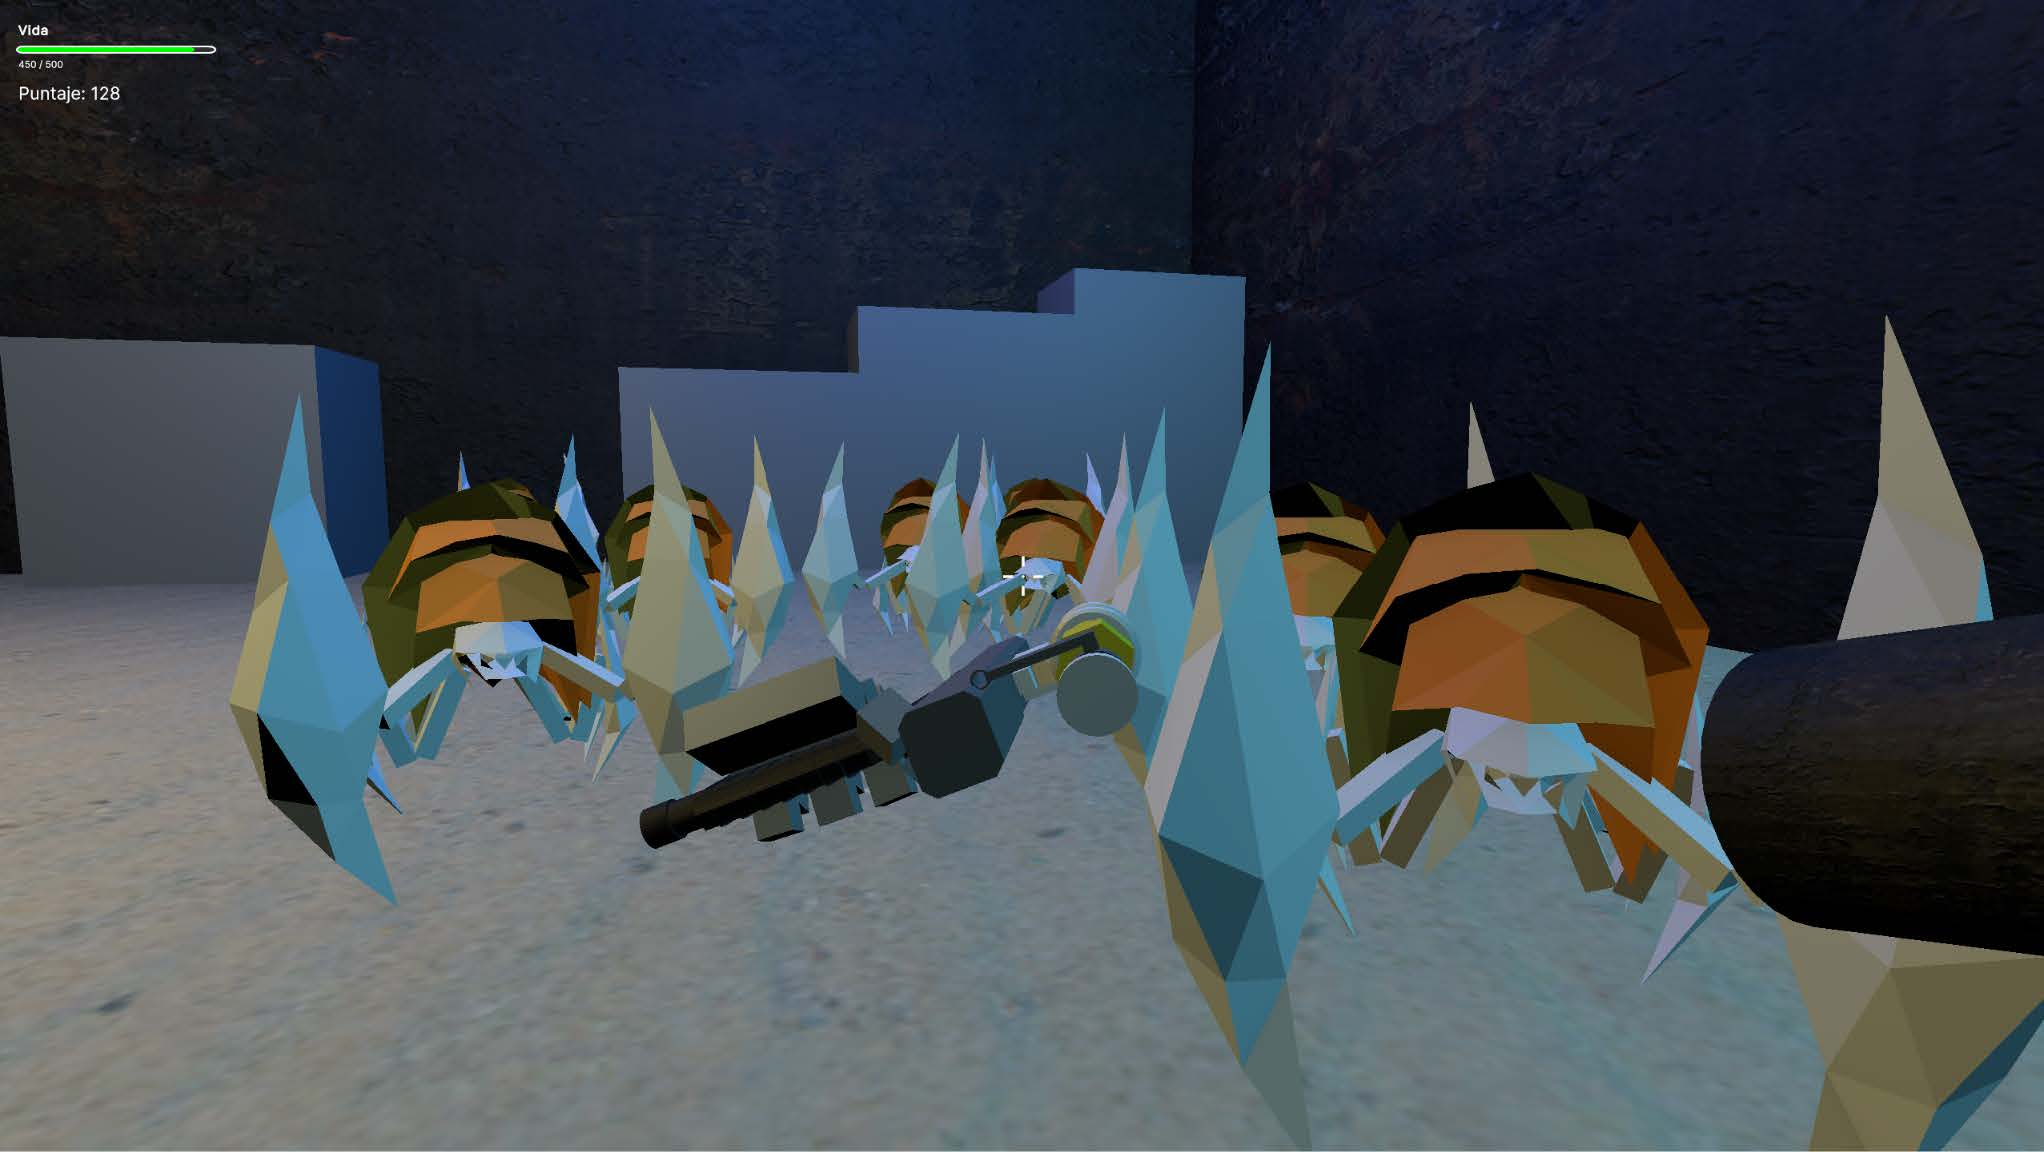
\includegraphics[width=0.7\textwidth]{figures/fpsingame.jpg}
\caption[Prototipo exploratorio FPS]{Prototipo exploratorio inicial del entorno FPS en Unity, desarrollado durante la primera fase del proyecto. Esta versión se utilizó para validar jugabilidad base y la viabilidad de integrar métricas en hardware local, pero fue descartada como entorno experimental principal por su alta complejidad y bajo control metodológico.}
\label{fig:fps_antiguo}
\end{figure}

\subsection{Descripción del Problema}

Actualmente, existe una percepción extendida ---tanto en la industria del videojuego como en la comunidad académica--- de que las inteligencias artificiales en videojuegos pueden o deberían ``aprender en tiempo real'' mientras interactúan con el jugador. Casos recientes como ARC Raiders han sido promocionados sugiriendo que los enemigos exhiben comportamientos emergentes aprendidos durante el gameplay, cuando la evidencia pública disponible indica que los modelos fueron entrenados durante el desarrollo y desplegados como políticas fijas.

Esta percepción genera una brecha entre la expectativa y la realidad técnica. Los paradigmas de aprendizaje automático más utilizados ---aprendizaje por refuerzo, neuroevolución, aprendizaje supervisado--- requieren volúmenes de datos y ciclos de entrenamiento que podrían exceder lo disponible en una sesión de juego contra un jugador humano. Sin embargo, esta brecha no ha sido cuantificada de forma sistemática bajo restricciones de hardware local.

Por otra parte, si bien existen herramientas y entornos para entrenar agentes de IA en videojuegos (como OpenAI Gym \cite{brockman2016openai}, Unity ML-Agents \cite{juliani2018mlagents} o Stable-Baselines3 \cite{raffin2021sb3}), estas están orientadas principalmente al proceso de entrenamiento offline, no a cuantificar la brecha entre los datos requeridos para entrenar y los datos que un jugador humano genera en una sesión real. Esta cuantificación resulta necesaria para determinar la viabilidad del aprendizaje en tiempo real.

El problema central que aborda este proyecto radica en la ausencia de evidencia experimental que cuantifique la viabilidad del aprendizaje de IA en tiempo real bajo restricciones de ejecución local, y en la necesidad de explorar alternativas ---como la adaptación por selección de especialistas pre-entrenados--- que ofrezcan adaptabilidad sin depender de entrenamiento online continuo.

\section{Propuesta de solución}

La propuesta de solución consiste en diseñar e implementar un entorno experimental que permita determinar, con evidencia cuantitativa, si es factible que una inteligencia artificial aprenda en tiempo real del jugador en un videojuego ejecutado en hardware local. Para ello, se construye una plataforma basada en un juego de turnos discretos (\textit{Knucklebones}), donde se entrenan tres paradigmas representativos de IA y se mide rigurosamente el costo de dicho entrenamiento, contrastándolo con los datos que un jugador humano genera en una sesión real.

El proyecto plantea dos líneas complementarias:

\begin{enumerate}
    \item \textbf{Cuantificación de la viabilidad del aprendizaje en tiempo real}: entrenar tres paradigmas de IA (aprendizaje por refuerzo, neuroevolución, aprendizaje supervisado destilado) de forma offline, midiendo los datos requeridos, el tiempo de entrenamiento y los recursos computacionales consumidos. Estos datos permiten evaluar la brecha entre los requisitos de cada paradigma y lo disponible en una sesión de juego real contra un jugador humano, determinando si el aprendizaje en tiempo real es viable o no.
    \item \textbf{Adaptación por selección como alternativa}: dado que la hipótesis inicial sugiere que el aprendizaje en tiempo real podría no ser viable con los paradigmas convencionales, se diseña e implementa un mecanismo de adaptación que no requiera reentrenamiento en tiempo de ejecución, basado en perfilado del oponente (clustering no supervisado) y selección de especialistas pre-entrenados. Este mecanismo se evalúa como alternativa práctica al entrenamiento online continuo.
\end{enumerate}

Para ello, se emplea el motor de desarrollo Unity como entorno de ejecución de reglas, junto con una arquitectura modular diseñada desde el inicio con separación estricta entre el motor del juego (responsable de reglas y transición de estado) y los agentes de IA (responsables exclusivamente de la selección de acciones). Un middleware HTTP/JSON permite la comunicación entre ambas capas. Esta separación modular fue una decisión de diseño planificada, no una limitación descubierta durante el desarrollo.

El sistema incluye instrumentación capaz de registrar métricas tales como latencia de decisión, carga computacional, tiempo de entrenamiento y tamaño de modelo. Estas métricas permiten evaluar de manera objetiva tanto el desempeño de cada enfoque como su costo, determinando su viabilidad bajo restricciones de hardware local.


La ejecución local en hardware convencional garantiza accesibilidad y reduce dependencia de recursos remotos. El diseño modular permite incorporar nuevos agentes o configuraciones experimentales con bajo costo adicional.

\subsection{Separación entre entrenamiento y ejecución}

Desde el diseño inicial del proyecto se estableció una arquitectura modular que separa la lógica del videojuego de los agentes de IA. El videojuego se mantiene como entorno estable que expone estado y recibe acciones, mientras que el entrenamiento se realiza fuera del motor utilizando un entorno equivalente tipo \textit{Gym} \cite{brockman2016openai}. Esta decisión de diseño responde a criterios de reproducibilidad, trazabilidad y eficiencia experimental.

El entorno equivalente permite ejecutar partidas a alta velocidad, generar datasets y entrenar modelos con mayor eficiencia, manteniendo consistencia con las reglas del juego y conservando la ejecución en hardware local. Esta separación no contradice el objetivo de evaluar la viabilidad del aprendizaje en tiempo real; por el contrario, permite medirla de forma rigurosa: si el entrenamiento offline ---en condiciones óptimas de velocidad y volumen de datos--- ya requiere órdenes de magnitud más datos de los disponibles en una sesión real, el entrenamiento en tiempo real durante la partida resulta inviable.

De esta manera, el sistema mantiene equivalencia funcional entre el entorno de entrenamiento y el entorno de evaluación, garantizando la validez experimental de los resultados obtenidos.

\section{Justificación de la propuesta}

El desarrollo de este proyecto se justifica por la necesidad de responder, con evidencia experimental, a una pregunta que la industria del videojuego y la comunidad académica asumen implícitamente pero no han cuantificado: ¿es viable que una inteligencia artificial aprenda en tiempo real dentro de un videojuego ejecutado en hardware local?

\textbf{Desde un punto de vista técnico}, la propuesta aborda esta pregunta mediante la medición rigurosa del costo de entrenamiento de tres paradigmas representativos (aprendizaje por refuerzo, neuroevolución, aprendizaje supervisado), cuantificando los datos, el tiempo y los recursos requeridos, y contrastándolos con lo disponible en una sesión real. La separación modular entre juego y agentes permite aislar el rendimiento del aprendizaje de factores externos, y el diseño del sistema habilita la evaluación de alternativas como la adaptación por selección.

\textbf{En términos de reproducibilidad}, la evaluación y el entrenamiento se realizan localmente en hardware doméstico, sin requerir infraestructura externa. Esto garantiza que los resultados puedan ser replicados por otros investigadores con recursos similares y elimina dependencias de servicios en la nube.

\textbf{Funcionalmente}, el sistema incluye instrumentación integrada que registra no solo el desempeño del agente durante el juego (winrate, latencia), sino también el costo del proceso de aprendizaje (tiempo de entrenamiento, datos requeridos, tamaño de modelo). Esta doble medición permite un análisis de viabilidad fundamentado en evidencia.

\textbf{Desde una perspectiva de investigación}, este proyecto contribuye con evidencia cuantitativa sobre una pregunta que, si bien es relevante tanto para la industria del videojuego como para cualquier dominio que requiera adaptación en tiempo real con recursos limitados, ha sido poco abordada de forma experimental: ¿cuánto cuesta realmente que una IA aprenda, y es posible hacerlo con los datos que genera un usuario en una sesión real?

\section{Objetivos}

\subsection{Objetivo General}

Evaluar el rendimiento y desempeño del aprendizaje de distintas inteligencias artificiales en un entorno de videojuego ejecutado completamente offline, cuantificando la brecha entre los requisitos de entrenamiento de tres paradigmas representativos y los datos disponibles en una sesión real contra un jugador humano, con el fin de determinar la viabilidad del aprendizaje en tiempo real y evaluar la adaptación por selección de especialistas pre-entrenados como alternativa práctica, sin depender de infraestructura en la nube.

\section{Alcance y limitaciones}

El trabajo abarca los siguientes elementos:

\begin{itemize}
    \item Diseño e implementación de una arquitectura modular que separa el videojuego de los agentes de IA.
    \item Entrenamiento de especialistas en tres paradigmas: PPO (aprendizaje por refuerzo), NEAT (neuroevolución) y DT (destilación por \textit{Behavior Cloning}).
    \item Medición del costo de entrenamiento de cada paradigma (datos, tiempo, recursos).
    \item Análisis de la brecha entre los datos requeridos y los disponibles en una sesión contra un jugador humano.
    \item Implementación de un mecanismo de adaptación por selección (KMeans + response table + especialistas).
    \item Integración del sistema completo en Unity mediante middleware HTTP/JSON.
\end{itemize}

Como limitaciones deliberadas:

\begin{itemize}
    \item No se implementa entrenamiento online completo dentro del motor del juego. Los resultados documentan cuantitativamente por qué dicho entrenamiento no es viable con los paradigmas evaluados.
    \item La estimación de datos disponibles en una sesión humana (10--100 partidas) es un supuesto operativo derivado de observación práctica, no un estudio formal de comportamiento de usuario.
    \item Los oponentes de entrenamiento y evaluación son heurísticos diseñados, no jugadores humanos reales.
    \item El entorno experimental es un juego de reglas simples (Knucklebones); la generalización a dominios más complejos queda como trabajo futuro.
\end{itemize}

\subsection{Objetivos Específicos}
\begin{itemize}
    \item Diseñar una arquitectura modular que permita incorporar y evaluar diferentes enfoques de inteligencia artificial sin modificar las reglas del videojuego.
    \item Implementar un prototipo funcional basado en un videojuego de turnos discretos que opere como plataforma de prueba para la ejecución y evaluación reproducible de agentes.
    \item Entrenar y evaluar tres paradigmas de aprendizaje ---aprendizaje por refuerzo (PPO), neuroevolución (NEAT) y aprendizaje supervisado destilado (DT)--- midiendo el costo de entrenamiento en términos de datos requeridos, tiempo y recursos computacionales.
    \item Cuantificar la brecha entre los requisitos de entrenamiento de cada paradigma y los datos disponibles en una sesión real contra un jugador humano, para determinar la viabilidad del aprendizaje en tiempo real.
    \item Implementar y evaluar un mecanismo de adaptación por selección de especialistas pre-entrenados como alternativa al entrenamiento online continuo.
    \item Integrar los agentes en el videojuego Unity mediante un middleware desacoplado, verificando la viabilidad operativa del sistema completo.
\end{itemize}

\subsection{Descripción de actividades}

\begin{itemize}

    \item \textbf{Diseñar una arquitectura modular para agentes intercambiables.}
    \begin{itemize}
        \item Diseño de la estructura modular del sistema y definición de interfaz estado/acción.
        \item Elaboración de esquemas lógicos y diagramas de componentes.
        \item Definición de flujos para integración de agentes y centralización de extracción de características.
    \end{itemize}

    \item \textbf{Desarrollar el prototipo de videojuego como entorno de evaluación.}
    \begin{itemize}
        \item Construcción del entorno base del juego seleccionado.
        \item Implementación del protocolo de observación por turno y aplicación de acciones.
        \item Aseguramiento de condiciones de control experimental (semillas, registro estructurado).
    \end{itemize}

    \item \textbf{Entrenar y medir el costo de aprendizaje de cada paradigma.}
    \begin{itemize}
        \item Entrenamiento de especialistas PPO mediante aprendizaje por refuerzo con entorno acelerado.
        \item Entrenamiento de especialistas NEAT mediante neuroevolución con evaluación multi-seed.
        \item Destilación de PPO a árboles de decisión mediante \textit{Behavior Cloning}.
        \item Registro de datos requeridos, tiempo de entrenamiento y recursos computacionales por cada paradigma.
    \end{itemize}

    \item \textbf{Cuantificar la brecha de viabilidad para entrenamiento en tiempo real.}
    \begin{itemize}
        \item Estimación de los datos disponibles en una sesión real contra un jugador humano.
        \item Cálculo de la relación entre datos requeridos y datos disponibles por paradigma.
        \item Análisis de convergencia con datos limitados (evidencia de entrenamiento insuficiente).
    \end{itemize}

    \item \textbf{Implementar y evaluar el mecanismo de adaptación por selección.}
    \begin{itemize}
        \item Entrenamiento de perfilador KMeans con datos de oponentes heurísticos.
        \item Construcción de tablas de respuesta por evaluación de especialistas por cluster.
        \item Evaluación comparativa del sistema adaptativo frente a generalistas fijos (\textit{ablation study}).
    \end{itemize}

    \item \textbf{Integrar el sistema completo en el videojuego Unity.}
    \begin{itemize}
        \item Implementación de middleware HTTP/JSON para comunicación Unity--Python.
        \item Verificación de equivalencia funcional entre entorno de simulación y motor de juego.
        \item Medición de latencia operativa del sistema integrado.
    \end{itemize}

\end{itemize}

\section{Descripción de los Aspectos Fundamentales de la Metodología Utilizada}

La presente investigación se enmarcó dentro del paradigma de la investigación aplicada, combinando elementos de análisis experimental, diseño iterativo de software y evaluación comparativa. Debido a la naturaleza técnica del proyecto, que implicó implementar un entorno de evaluación reproducible, instrumentado y controlado para medir de forma cuantificable el comportamiento y el costo computacional de agentes de IA bajo condiciones homogéneas, se adoptó una metodología de carácter evolutivo y orientada a prototipos.

El enfoque metodológico se fundamentó en tres pilares principales:

\begin{itemize}
    \item \textbf{Investigación exploratoria y revisión técnica:} permitió comprender el estado actual de las tecnologías involucradas, incluyendo IA para videojuegos, modularidad de software, instrumentación y limitaciones de hardware local.
    \item \textbf{Desarrollo incremental de prototipos:} el videojuego y los módulos del sistema fueron construidos de manera progresiva, incorporando funcionalidades esenciales en ciclos iterativos. Este enfoque facilitó la validación temprana de componentes, redujo riesgos asociados a la complejidad del sistema y permitió evaluar continuamente la factibilidad técnica del proyecto.
    \item \textbf{Experimentación y análisis de rendimiento:} los enfoques de IA fueron evaluados mediante métricas cuantitativas, incluyendo latencia de decisión, uso de CPU/memoria, estabilidad y métricas de desempeño dentro del juego. Esta fase permitió comparar enfoques bajo condiciones homogéneas y completamente offline.
\end{itemize}

La elección de una metodología evolutiva respondió a la incertidumbre inherente al desarrollo de sistemas de IA y al nivel de riesgo técnico asociado a integración, medición y control experimental. Este enfoque permitió ajustar el diseño del sistema de forma continua y corregir desviaciones durante el avance de la investigación.

En la primera etapa se desarrolló un levantamiento del marco tecnológico y conceptual. Luego se diseñó e implementó una arquitectura modular que soporta la integración de agentes y registro de métricas. Posteriormente, se construyó el prototipo funcional como plataforma de pruebas, sobre el cual se integraron y evaluaron distintos enfoques de IA. Finalmente, se realizó un análisis comparativo de resultados con el fin de determinar la factibilidad técnica y operativa de los enfoques evaluados en un entorno de videojuego ejecutado completamente en hardware local.

De esta manera, la metodología seleccionada garantizó una progresión controlada del proyecto, favoreció la validación temprana de hipótesis y aseguró que los objetivos planteados pudieran ser alcanzados mediante un proceso sistemático, reproducible y fundamentado en evidencia experimental.

\section{Composición del informe}

El presente trabajo se encuentra dividido en seis capítulos. A continuación se describe brevemente el contenido de cada uno de ellos.

\begin{enumerate}
    \item \textbf{Introducción:} presentación del problema, objetivos, alcance y metodología general del trabajo.
    \item \textbf{Bases Teóricas:} fundamentos sobre IA en videojuegos, aprendizaje automático, distinción entre aprendizaje online y adaptación por selección, costos de entrenamiento y reproducibilidad experimental.
    \item \textbf{Estado del Arte:} revisión de enfoques existentes en la industria y la academia, con énfasis en la viabilidad del aprendizaje en tiempo real y las prácticas de adaptación utilizadas.
    \item \textbf{Desarrollo del trabajo:} diseño e implementación de la plataforma, arquitectura modular, instrumentación, flujo experimental y criterios de viabilidad para entrenamiento en tiempo real.
    \item \textbf{Resultados:} medición de costos de aprendizaje, análisis de brecha de datos, evaluación de sistemas adaptativos, discusión de viabilidad y comparación de paradigmas.
    \item \textbf{Conclusiones:} síntesis de hallazgos sobre viabilidad del aprendizaje, validación de la adaptación por selección y proyecciones.
\end{enumerate}

Además, al final del informe se adjuntan las referencias bibliográficas utilizadas en el proceso de investigación.
\vfill

\chapter{Bases Teóricas y Antecedentes}\label{cap:marco_teorico}
El presente capítulo tiene por finalidad describir los fundamentos conceptuales, tecnológicos y metodológicos asociados al uso de inteligencia artificial aplicada a videojuegos, con énfasis en la evaluación del rendimiento y desempeño del aprendizaje bajo restricciones de ejecución local. Se presentan conceptos clave sobre IA en videojuegos, aprendizaje automático, la distinción entre aprendizaje online y adaptación por selección, los costos asociados al entrenamiento de modelos, y nociones de modularidad y reproducibilidad experimental.

A través de esta revisión se establece un marco conceptual que permite comprender: (i) por qué los videojuegos constituyen entornos relevantes para evaluar el aprendizaje de agentes, (ii) qué técnicas de IA resultan factibles bajo recursos computacionales limitados, (iii) cuáles son los costos reales del proceso de aprendizaje en cada paradigma, y (iv) qué alternativas existen cuando el entrenamiento en tiempo real no es viable.

\section{Inteligencia Artificial en Videojuegos}

La inteligencia artificial (IA) ha sido un componente central en el desarrollo de videojuegos desde sus primeras generaciones \cite{yannakakis2018ai}. Su propósito principal es controlar el comportamiento de personajes no jugadores (\textit{Non-Player Characters}, NPC), administrar dinámicas del entorno y ofrecer experiencias desafiantes y coherentes para el jugador humano.

A diferencia de otras áreas de la IA, en videojuegos la toma de decisiones suele estar condicionada por restricciones de tiempo real, estabilidad del sistema y criterios de diseño (\textit{game design}); por lo tanto, la IA debe ser no solo efectiva, sino también controlable, predecible en su estructura y suficientemente interpretable para evitar comportamientos indeseados o desbalanceados.

Tradicionalmente, la IA en videojuegos se ha implementado mediante enfoques deterministas y basados en reglas, entre los cuales destacan:

\begin{itemize}
    \item Máquinas de estados finitos (FSM).
    \item Árboles de decisión.
    \item Árboles de comportamiento (\textit{Behavior Trees}).
    \item Sistemas basados en reglas y heurísticas.
\end{itemize}

Estos modelos presentan ventajas relevantes: bajo costo computacional, facilidad de depuración y control explícito del comportamiento. Sin embargo, su principal limitación es la ausencia de adaptación genuina: el agente no modifica su política a partir de la experiencia, y su comportamiento tiende a volverse predecible ante jugadores recurrentes, lo que puede afectar la rejugabilidad.

\subsection{IA determinista vs. IA adaptativa}

En términos generales, puede distinguirse entre:

\begin{itemize}
    \item \textbf{IA determinista:} ejecuta políticas fijas predefinidas (por ejemplo, reglas o árboles con parámetros constantes), sin mecanismos de actualización basados en datos.
    \item \textbf{IA adaptativa:} modifica su comportamiento en función del jugador o del historial de interacción. Esta adaptación puede lograrse mediante reglas dinámicas diseñadas por el desarrollador o mediante técnicas de aprendizaje automático.
\end{itemize}

Una consideración relevante para esta investigación es que el término ``adaptativo'' no implica necesariamente entrenamiento profundo en tiempo real. En videojuegos, un enfoque adaptativo puede consistir en selección de estrategias, ajuste de parámetros o cambio de política en función de patrones observables, manteniendo control de diseño y costo computacional acotado.

En el contexto de este trabajo, la adaptatividad se aborda desde una perspectiva centrada en el costo del aprendizaje: se investiga cuánto cuesta entrenar cada paradigma y se evalúa la adaptación por selección como alternativa al entrenamiento en tiempo real.

\subsection{Aprendizaje online pleno vs. adaptación online por selección}

Una distinción central para esta investigación es la diferencia entre dos formas de lograr comportamiento adaptativo en tiempo de ejecución:

\begin{itemize}
    \item \textbf{Aprendizaje online pleno}: consiste en actualizar los parámetros o pesos del modelo \textit{durante la partida}, utilizando las interacciones en curso como datos de entrenamiento. Esto requiere ejecutar algoritmos de optimización (retropropagación, evaluación de fitness, etc.) en tiempo real, con los costos computacionales y de datos asociados. Ejemplos: fine-tuning de una red neuronal con los turnos jugados, evolución de genomas con las partidas observadas.

    \item \textbf{Adaptación online por selección}: no se actualizan los pesos del modelo en runtime. En su lugar, se mantiene un catálogo de políticas pre-entrenadas y se selecciona la más adecuada en función de un perfil del oponente construido en tiempo real. Esto requiere únicamente inferencia (microsegundos) y un módulo de perfilado ligero (por ejemplo, clustering), sin costo de entrenamiento durante la partida.
\end{itemize}

Esta distinción es relevante porque el término ``IA adaptativa'' en videojuegos frecuentemente se utiliza sin precisar cuál de estos dos mecanismos se está describiendo. El presente trabajo evalúa experimentalmente la viabilidad del primero y propone el segundo como alternativa demostrada.

\section{Aprendizaje Automático (\textit{Machine Learning})}

El \textit{Machine Learning} (ML) es una rama de la IA basada en la idea de que un sistema puede aprender patrones a partir de datos, mejorar su rendimiento con la experiencia y generalizar hacia nuevas situaciones sin ser programado explícitamente con reglas exhaustivas. En el contexto de videojuegos, el ML puede utilizarse para:

\begin{itemize}
    \item predecir acciones o preferencias del jugador,
    \item clasificar estilos de juego (por ejemplo, agresivo o defensivo),
    \item aprender políticas de decisión mediante interacción con el entorno,
    \item aproximar funciones de evaluación o comportamiento.
\end{itemize}

Las principales categorías de ML se describen a continuación.

\subsection{Aprendizaje supervisado}

El aprendizaje supervisado entrena un modelo utilizando ejemplos etiquetados $(x, y)$, donde $x$ representa un conjunto de características (\textit{features}) y $y$ una salida objetivo (clase o valor). En videojuegos, esto resulta útil cuando se dispone de datos registrados (por ejemplo, decisiones por turno) y se busca:

\begin{itemize}
    \item predecir una acción a partir del estado,
    \item imitar una política base (aprendizaje por imitación),
    \item clasificar eventos o patrones del juego.
\end{itemize}

Una ventaja clave del aprendizaje supervisado es su eficiencia tanto en entrenamiento como en inferencia (dependiendo del modelo), además de su potencial interpretabilidad en modelos como los árboles de decisión.

\subsection{Aprendizaje no supervisado}

El aprendizaje no supervisado busca identificar estructura en datos sin etiquetas explícitas. Su aplicación en videojuegos incluye:

\begin{itemize}
    \item agrupamiento (\textit{clustering}) de jugadores según patrones de comportamiento,
    \item reducción de dimensionalidad,
    \item detección de anomalías o estilos de juego.
\end{itemize}

En el contexto de IA adaptativa, un modelo no supervisado puede actuar como módulo auxiliar que detecta perfiles y gatilla cambios de estrategia, sin necesariamente ejecutar directamente la política de juego.

\subsection{Aprendizaje por refuerzo (\textit{Reinforcement Learning})}

El aprendizaje por refuerzo (RL) modela el problema como un agente que interactúa con un entorno y recibe recompensas, aprendiendo una política $\pi(a \mid s)$ que maximiza el retorno esperado \cite{sutton2018reinforcement}. Sus elementos básicos son:

\begin{itemize}
    \item \textbf{Agente:} entidad que selecciona acciones.
    \item \textbf{Entorno:} sistema con el que el agente interactúa.
    \item \textbf{Estado $s$:} representación de la situación actual.
    \item \textbf{Acción $a$:} decisión aplicada al entorno.
    \item \textbf{Recompensa $r$:} retroalimentación numérica que guía el aprendizaje.
    \item \textbf{Política $\pi$:} regla de decisión del agente.
\end{itemize}

RL es especialmente relevante en videojuegos por su naturaleza secuencial y por la posibilidad de generar episodios de interacción. No obstante, en escenarios de ejecución local, el entrenamiento de RL puede resultar costoso en tiempo y recursos computacionales, por lo que suele requerir simulaciones aceleradas o entrenamiento fuera del motor del juego para mantener un ciclo de iteración razonable.

\section{Videojuegos como entornos de evaluación experimental}

Los videojuegos pueden funcionar como entornos experimentales adecuados para evaluar agentes por diversas razones:

\begin{itemize}
    \item \textbf{Entornos controlados:} reglas explícitas y estados formalizables.
    \item \textbf{Interacciones repetibles:} posibilidad de re-ejecutar episodios con semillas controladas.
    \item \textbf{Retroalimentación inmediata:} métricas observables por turno o por episodio.
    \item \textbf{Simulación acelerada:} en juegos por turnos, es posible ejecutar múltiples episodios rápidamente fuera del motor.
\end{itemize}

En esta investigación se prioriza un entorno con reglas simples y estado completamente observable, de modo que la comparación entre agentes sea atribuible al enfoque de IA y no a factores externos como percepción parcial compleja, navegación continua o variabilidad no controlada.

\section{Ejecución local, modularidad e integración}

La ejecución local impone restricciones prácticas relacionadas con capacidad de CPU/GPU, memoria disponible, estabilidad del proceso y latencias tolerables. En este escenario, el diseño arquitectónico se vuelve crítico para asegurar viabilidad y comparabilidad.

\subsection{Separación de responsabilidades y arquitectura modular}

Un principio de ingeniería relevante es la separación de responsabilidades (\textit{separation of concerns}): el juego debe encargarse de ejecutar reglas y transiciones de estado, mientras que los agentes deben encargarse exclusivamente de seleccionar acciones. Esta separación habilita una arquitectura \textit{plug-and-play}, donde distintos agentes pueden intercambiarse sin modificar el núcleo del videojuego.

En esta investigación, la modularidad se considera un requisito metodológico, dado que permite:

\begin{itemize}
    \item comparar agentes bajo reglas idénticas,
    \item centralizar el cálculo de características para evitar inconsistencias,
    \item registrar métricas de forma uniforme,
    \item reducir acoplamiento y complejidad de mantenimiento.
\end{itemize}

Este principio se operacionaliza mediante el concepto de \textit{juego inmutable}, donde el motor se limita a ejecutar reglas y transiciones de estado, mientras que cualquier lógica específica de IA permanece desacoplada y reemplazable.

\subsection{Entornos equivalentes tipo \textit{Gym}}

Debido a restricciones de tiempo y costo de iteración, resulta práctico entrenar o evaluar ciertos modelos fuera del motor del juego mediante un entorno equivalente tipo \textit{Gym} \cite{brockman2016openai}. Este entorno replica las reglas relevantes y expone una interfaz estándar (observación, acción, recompensa y terminación), permitiendo ejecutar episodios a mayor velocidad y generar datasets de forma eficiente.

Este enfoque es coherente con la ejecución local, ya que tanto el entrenamiento como la evaluación continúan realizándose en el hardware del usuario, pero desacoplados del motor, lo cual facilita la instrumentación y la reproducibilidad.

Para preservar la validez experimental, el entorno equivalente debe cumplir equivalencia funcional respecto al motor del juego. En términos prácticos, esto implica que, para una misma transición estado--acción, ambos entornos produzcan el mismo estado resultante. Este criterio puede verificarse mediante trazas de referencia (\textit{golden logs}) y pruebas sistemáticas de transición.

\section{Reproducibilidad experimental e instrumentación}

En trabajos experimentales, la reproducibilidad es fundamental para validar resultados y comparar enfoques. En el contexto de videojuegos, esto requiere controlar fuentes de aleatoriedad y asegurar trazabilidad completa de ejecuciones.

\subsection{Semillas y control de aleatoriedad}

El uso de semillas permite controlar generadores de números aleatorios (RNG) tanto en el entorno como en los agentes. Al fijar una semilla, una secuencia de eventos aleatorios (por ejemplo, valores de dados o desempates) puede repetirse, habilitando comparaciones justas entre agentes bajo condiciones homogéneas.

\subsection{Registro estructurado (\textit{logging})}

El registro estructurado de decisiones por turno permite:

\begin{itemize}
    \item reconstruir partidas completas,
    \item analizar causas de decisiones,
    \item medir latencia y costo computacional,
    \item construir datasets para entrenamiento supervisado,
    \item comparar estabilidad y variabilidad entre ejecuciones.
\end{itemize}

En este trabajo, el registro estructurado se plantea como componente metodológico central, ya que actúa como evidencia experimental y soporte para el análisis cuantitativo.

\section{Costos computacionales y de datos del entrenamiento}

El proceso de entrenamiento de modelos de aprendizaje automático implica costos que varían significativamente según el paradigma utilizado. Comprender estos costos es fundamental para evaluar la viabilidad de cada enfoque bajo restricciones de ejecución local.

\subsection{Aprendizaje por refuerzo}

El entrenamiento de agentes por RL requiere que el agente interactúe con el entorno durante cientos de miles o millones de pasos (\textit{timesteps}). Algoritmos como PPO \cite{schulman2017ppo} utilizan rollouts (secuencias de interacción) para estimar gradientes de política. El volumen de datos necesario depende de la complejidad del entorno, pero en la práctica se requieren entre $10^5$ y $10^7$ timesteps para juegos simples \cite{sutton2018reinforcement}. Este volumen es generado por el propio proceso de entrenamiento interactuando con un simulador, no por jugadores humanos.

\subsection{Neuroevolución}

Los algoritmos evolutivos como NEAT \cite{stanley2002neat} evalúan poblaciones completas de candidatos (genomas) durante múltiples generaciones. El costo total se expresa como: generaciones $\times$ tamaño de población $\times$ episodios por genoma. Con poblaciones de 150 individuos, 300 generaciones y 50--100 episodios por evaluación, el volumen total de episodios puede alcanzar millones. A diferencia de RL, la evaluación de cada individuo es independiente y paralelizable, pero el volumen total sigue siendo elevado.

\subsection{Aprendizaje supervisado (destilación)}

El aprendizaje supervisado por imitación (\textit{Behavior Cloning}) \cite{hussein2017imitation} es computacionalmente ligero en la fase de entrenamiento del modelo (segundos), pero depende de un dataset generado previamente. Este dataset requiere un teacher ya entrenado (por ejemplo, un agente PPO), lo que traslada el costo a una etapa anterior. El volumen de datos etiquetados necesario es del orden de $10^5$--$10^6$ muestras para lograr fidelidad superior al 90\%.

\subsection{Implicaciones para el aprendizaje en tiempo real}

Los costos descritos permiten anticipar que el entrenamiento en tiempo real ---donde los datos provienen exclusivamente de la interacción con un jugador humano durante una sesión de juego--- enfrenta una limitación fundamental: el jugador humano genera órdenes de magnitud menos datos de los requeridos por cualquiera de estos paradigmas. Esta brecha se cuantifica experimentalmente en el Capítulo~\ref{cap:aplicacion}.

\section{Paradigmas de aprendizaje evaluados en el proyecto}

Con el objetivo de evaluar el rendimiento y desempeño del aprendizaje bajo restricciones locales, se seleccionaron tres paradigmas representativos que cubren distintas familias de aprendizaje automático y presentan costos de entrenamiento contrastados:

\begin{itemize}
    \item \textbf{Aprendizaje por refuerzo (PPO):} el agente aprende una política mediante interacción con el entorno, optimizando el retorno esperado. Representa el paradigma de mayor costo de datos.
    \item \textbf{Neuroevolución (NEAT):} el agente evoluciona mediante algoritmos genéticos que optimizan la topología y pesos de redes neuronales. Representa un costo intermedio con alta paralelizabilidad.
    \item \textbf{Aprendizaje supervisado destilado (DT):} el agente aprende por imitación de un teacher previamente entrenado (PPO), produciendo un modelo ligero e interpretable. Representa el menor costo de entrenamiento directo, pero depende de un teacher.
\end{itemize}

Adicionalmente, el proyecto emplea componentes auxiliares que no constituyen paradigmas de aprendizaje independientes:

\begin{itemize}
    \item \textbf{Heurísticas:} políticas deterministas diseñadas manualmente que sirven como baseline y como oponentes de entrenamiento.
    \item \textbf{Perfilador KMeans:} módulo no supervisado que clasifica el estilo del oponente para habilitar la selección de especialistas.
\end{itemize}

Esta selección permite estudiar la relación entre desempeño y costo computacional, y cuantificar qué se obtiene realmente al incorporar aprendizaje respecto a una política base. La combinación de los tres paradigmas con el perfilador KMeans conforma los sistemas adaptativos evaluados.

\section{Métricas de evaluación}

Para medir el rendimiento y desempeño del aprendizaje se requieren métricas en dos niveles complementarios: el costo del proceso de aprendizaje y el desempeño del agente resultante.

\subsection{Métricas de costo del aprendizaje (nivel primario)}

\begin{itemize}
    \item \textbf{Datos requeridos:} volumen de muestras, episodios o timesteps necesarios para que el modelo converja a una política funcional.
    \item \textbf{Tiempo de entrenamiento:} duración del proceso de entrenamiento medida en segundos de reloj (\textit{wall time}).
    \item \textbf{Uso de CPU y memoria:} costo de recursos computacionales durante el entrenamiento.
    \item \textbf{Tamaño del modelo resultante:} espacio en disco del artefacto entrenado.
    \item \textbf{Brecha de datos:} relación entre los datos requeridos y los disponibles en una sesión real contra un jugador humano.
\end{itemize}

\subsection{Métricas de desempeño del agente (nivel secundario)}

\begin{itemize}
    \item \textbf{Tasa de victoria (\textit{winrate}):} proporción de partidas ganadas, que confirma que el agente entrenado es funcional.
    \item \textbf{Diferencial de puntaje:} diferencia promedio entre el puntaje del agente y el del oponente.
    \item \textbf{Estabilidad:} variabilidad de resultados entre ejecuciones repetidas.
    \item \textbf{Latencia de decisión:} tiempo requerido para seleccionar una acción por turno (relevante para la viabilidad operativa).
\end{itemize}

El análisis conjunto de ambos niveles permite estudiar el compromiso (\textit{trade-off}) entre el costo del aprendizaje y la calidad del agente resultante, determinando si la inversión en entrenamiento se justifica y bajo qué condiciones es viable.


\chapter{Estado del Arte}\label{cap:estado_del_arte}
El presente capítulo revisa los enfoques actuales utilizados para implementar inteligencia artificial en videojuegos, tanto en contextos académicos como industriales. Se analizan técnicas deterministas, enfoques basados en aprendizaje automático y mecanismos de adaptación al jugador, con especial atención a la viabilidad del aprendizaje en tiempo real y a las alternativas implementadas en la práctica bajo restricciones de hardware local.

\section{IA clásica en videojuegos comerciales}

La mayoría de los videojuegos comerciales continúan utilizando modelos deterministas como máquinas de estados finitos (FSM), árboles de comportamiento y sistemas basados en reglas \cite{yannakakis2018ai}. Estos enfoques permiten un control preciso del comportamiento, bajo consumo computacional y alta estabilidad en tiempo real.

Ejemplos representativos incluyen la saga \textit{Halo} (Bungie/343 Industries), donde los enemigos utilizan árboles de comportamiento para coordinar tácticas de grupo; \textit{F.E.A.R.} (Monolith, 2005), reconocido por su sistema de planificación GOAP (\textit{Goal-Oriented Action Planning}); y \textit{The Last of Us} (Naughty Dog, 2013), donde la IA de los compañeros emplea FSM con ajustes contextuales. En todos estos casos, la IA prioriza coherencia narrativa, controlabilidad y estabilidad sobre el aprendizaje autónomo. Su bajo costo computacional y facilidad de depuración los mantienen vigentes en producción comercial.

\section{Adaptación sin aprendizaje online pleno}

En varios títulos comerciales se implementan mecanismos de adaptación al jugador que, a pesar de generar la percepción de aprendizaje, no actualizan pesos de modelos durante la ejecución. A continuación se presentan tres casos representativos.

\subsection{Caso Alien: Isolation (Creative Assembly, 2014)}

El Xenomorfo de Alien: Isolation no entrena un modelo de aprendizaje automático. En su lugar, detecta patrones del jugador y desbloquea contramedidas predefinidas. Si el jugador se esconde frecuentemente debajo de mesas, el Alien incrementa la probabilidad de buscar en esas ubicaciones. Este mecanismo constituye adaptación por reglas condicionales, no por aprendizaje.

\subsection{Caso Metal Gear Solid V (Konami, 2015)}

En MGSV, los soldados enemigos reaccionan a tendencias del jugador: muchos disparos a la cabeza provocan que los soldados usen cascos; jugar frecuentemente de noche resulta en que los enemigos adquieran visores nocturnos. Este sistema representa un enfoque adaptativo basado en contadores y umbrales, sin componentes de aprendizaje automático.

\subsection{Síntesis: adaptación por diseño, no por entrenamiento}

Estos casos evidencian que la adaptación al jugador en videojuegos comerciales se implementa predominantemente mediante reglas condicionales, contadores y respuestas predefinidas por los diseñadores. No se actualizan pesos ni se ejecutan algoritmos de optimización en runtime. La adaptación se logra por diseño, no por aprendizaje.

\section{Machine Learning en desarrollo y despliegue offline}

\subsection{Caso ARC Raiders (Embark Studios)}

ARC Raiders, desarrollado por Embark Studios \cite{arcraiders2025site}, fue analizado como caso industrial contemporáneo asociado discursivamente a inteligencia artificial ``emergente''. La evidencia pública revisada sugiere que ARC Raiders emplea \textit{Machine Learning} en subsistemas específicos, particularmente locomoción o animación de ciertos enemigos, mediante entrenamiento realizado durante el desarrollo \cite{arcraiders2025interview}. Sin embargo, no se encontraron fuentes técnicas públicas que demuestren aprendizaje \textit{online} pleno o actualización de pesos durante la ejecución de las partidas. En consecuencia, el caso resulta más consistente con un esquema de entrenamiento \textit{offline} y despliegue en inferencia que con aprendizaje en tiempo real dentro del juego final \cite{arcraiders2025steam}.

Este caso ilustra una práctica frecuente en la industria: el uso de ML como herramienta de desarrollo, no como mecanismo de adaptación en tiempo de ejecución. La percepción pública de ``IA que aprende'' no corresponde necesariamente con la implementación técnica real del producto.

\subsection{Uso industrial de ML en videojuegos}

En la práctica industrial, el ML suele utilizarse para tareas específicas como análisis de comportamiento del jugador, generación procedural o balance dinámico, pero rara vez como entrenamiento autónomo en tiempo real dentro del juego final. Frameworks como Unity ML-Agents \cite{juliani2018mlagents} permiten entrenar agentes mediante interacción simulada, pero el entrenamiento se realiza en fase de desarrollo y los modelos resultantes se despliegan como políticas fijas.

\subsection{Síntesis de casos industriales}

En los casos industriales revisados en este trabajo no se observa actualización de pesos de modelos en tiempo de ejecución. La literatura académica coincide en que la IA en videojuegos comerciales privilegia el control de diseño y la estabilidad sobre el aprendizaje autónomo \cite{yannakakis2018ai}. La adaptación al jugador se resuelve, en los casos observados, mediante reglas predefinidas, contadores o políticas pre-entrenadas, no mediante entrenamiento continuo en runtime.

La Tabla~\ref{tab:estado_arte_casos} resume los enfoques de adaptación identificados en los casos analizados.

\begin{table}[H]
\centering
\caption{Resumen de enfoques de adaptación en casos industriales y académicos}
\begin{tabular}{llcc}
\hline
\textbf{Caso} & \textbf{Mecanismo} & \textbf{Aprendizaje online} & \textbf{Hardware} \\
\hline
Alien: Isolation & Reglas condicionales & No & Local \\
Metal Gear Solid V & Contadores y umbrales & No & Local \\
ARC Raiders & ML offline + inferencia & No & Local \\
AlphaGo / AlphaStar & RL masivo offline & No & TPUs/GPUs \\
\hline
\end{tabular}
\label{tab:estado_arte_casos}
\end{table}

Este patrón refuerza la pregunta central de esta investigación: ¿el aprendizaje en tiempo real no se implementa porque no es necesario, o porque no es viable? El presente trabajo aborda esta pregunta con evidencia experimental cuantitativa.

\section{Brecha entre logros académicos y despliegue real}

En entornos académicos, proyectos como AlphaGo \cite{silver2016mastering}, OpenAI Five y AlphaStar \cite{vinyals2019grandmaster} han demostrado la capacidad de agentes entrenados mediante RL para superar a expertos humanos en juegos complejos. No obstante, estos sistemas requieren infraestructura de cómputo masivo: AlphaStar utilizó 16 TPUs durante 44 días, y OpenAI Five requirió miles de GPUs durante meses. Estos volúmenes de cómputo son inalcanzables en hardware local convencional.

Un aspecto poco discutido en la literatura es que estos logros fueron alcanzados con entrenamiento offline masivo, no con aprendizaje durante la partida contra humanos. Los agentes resultantes son políticas fijas desplegadas para evaluación. Esto demuestra que incluso con recursos computacionales prácticamente ilimitados, el entrenamiento se realiza offline y se despliega como inferencia.

El aprendizaje por refuerzo (RL) ha mostrado resultados sobresalientes en entornos con reglas bien definidas. Algoritmos como Q-Learning, DQN \cite{mnih2015dqn} y PPO \cite{schulman2017ppo} han sido ampliamente utilizados en juegos discretos y simulaciones. Sin embargo, el entrenamiento requiere gran cantidad de episodios, lo que introduce una separación entre entrenamiento y despliegue.

\section{Adaptación basada en perfilado de jugador}

Otra línea relevante en el estado del arte es la adaptación basada en análisis del comportamiento del jugador \cite{yannakakis2013player}. Técnicas de clustering y clasificación se utilizan para detectar perfiles (por ejemplo, agresivo, defensivo, explorador), ajustando parámetros o seleccionando estrategias predefinidas.

Este enfoque presenta ventajas importantes:
\begin{itemize}
    \item Bajo costo computacional en runtime.
    \item Fácil integración con sistemas existentes.
    \item Control de diseño sobre las respuestas del sistema.
\end{itemize}

A diferencia del RL profundo, estos mecanismos permiten adaptación sin necesidad de entrenamiento masivo continuo, lo que los hace particularmente relevantes para ejecución local.

\section{Ejecución local versus infraestructura en nube}

La mayoría de los desarrollos avanzados en ML para videojuegos dependen de entrenamiento en la nube o en entornos de cómputo de alto rendimiento. Si bien esto permite modelos complejos, introduce dependencia de infraestructura externa y eleva los costos.

En contraste, la ejecución local impone restricciones que afectan directamente la viabilidad del aprendizaje:

\begin{itemize}
    \item Capacidad limitada de cómputo (CPU doméstico, GPU de gama media).
    \item Volumen de datos limitado a las interacciones con el usuario local.
    \item Necesidad de latencia baja para mantener la experiencia de juego.
    \item Ausencia de simuladores acelerados durante la partida real.
\end{itemize}

La literatura existente asume implícitamente que el entrenamiento en tiempo real en hardware local no es viable, pero esta suposición no ha sido cuantificada de forma experimental con paradigmas representativos. Este trabajo aborda esa carencia.

\section{Limitaciones identificadas en el estado del arte}

Del análisis realizado se desprenden las siguientes limitaciones:

\begin{itemize}
    \item Ausencia de cuantificación experimental de la brecha de datos entre entrenamiento offline y sesión real.
    \item Alta dependencia de infraestructura externa para entrenamiento en la mayoría de los trabajos académicos.
    \item Escasa distinción formal entre aprendizaje online pleno y adaptación por selección en la literatura de IA para videojuegos.
    \item Falta de evidencia empírica sobre qué ocurre cuando se intenta entrenar con el volumen de datos disponible en una sesión humana real.
\end{itemize}

\section{Posicionamiento del presente trabajo}

El presente proyecto se posiciona como una investigación experimental que busca:

\begin{itemize}
    \item Cuantificar el costo real del aprendizaje de tres paradigmas representativos (RL, neuroevolución, aprendizaje supervisado) en hardware local.
    \item Medir la brecha entre los datos requeridos por cada paradigma y los disponibles en una sesión contra un jugador humano.
    \item Evaluar la adaptación por selección de especialistas pre-entrenados como alternativa demostrable al entrenamiento online continuo.
    \item Contribuir con evidencia experimental sobre una pregunta relevante para la industria: ¿es viable que una IA aprenda en tiempo real dentro de un videojuego en hardware local?
\end{itemize}


\chapter{Desarrollo del Trabajo} \label{cap:metodologia}
El presente capítulo describe el diseño e implementación de la plataforma experimental desarrollada para evaluar el rendimiento y desempeño del aprendizaje de agentes de inteligencia artificial en un entorno de videojuego ejecutado localmente. Se detallan los componentes arquitectónicos, el flujo de comunicación entre módulos, la representación del estado, los mecanismos de registro, el protocolo experimental adoptado y los criterios de viabilidad considerados para evaluar la factibilidad del aprendizaje en distintas condiciones de ejecución.

\section{Arquitectura General del Sistema}

La plataforma se diseñó bajo una arquitectura modular con separación explícita entre el videojuego y los agentes de IA. Esta decisión responde a la necesidad de:

\begin{itemize}
    \item Mantener el juego como fuente única de verdad respecto a reglas.
    \item Permitir el intercambio de agentes sin modificar el motor.
    \item Centralizar la extracción de características.
    \item Garantizar comparabilidad experimental.
\end{itemize}

La arquitectura se compone de tres capas principales:

\begin{enumerate}
    \item \textbf{Videojuego (Unity):} ejecuta las reglas del juego, administra el estado y aplica las acciones.
    \item \textbf{Middleware local:} recibe el estado del juego, procesa la información, enruta la decisión hacia el agente activo y registra métricas.
    \item \textbf{Agentes IA intercambiables:} módulos independientes que implementan una interfaz común de decisión.
\end{enumerate}

Este diseño permite una estructura \textit{plug-and-play}, donde los agentes pueden reemplazarse sin alterar el núcleo del sistema. La Figura~\ref{fig:arquitectura_3capas} presenta la arquitectura general del sistema.

\begin{figure}[H]
\centering
\begin{tikzpicture}[
    block/.style={rectangle, draw, text width=3.8cm, minimum height=2cm, align=center, font=\small},
    arrow/.style={-{Stealth[length=3mm]}, thick},
    label/.style={font=\footnotesize, midway, fill=white, inner sep=1pt}
]
\node[block, fill=blue!15] (unity) {\textbf{Videojuego}\\(Unity / C\#)\\[3pt]Reglas, estado,\\UI, input humano};
\node[block, fill=orange!15, right=2cm of unity] (middleware) {\textbf{Middleware}\\(Python / Flask)\\[3pt]Features, routing,\\logging, métricas};
\node[block, fill=green!15, right=2cm of middleware] (agentes) {\textbf{Agentes IA}\\(Python)\\[3pt]PPO, NEAT, DT,\\KMeans, Heurísticos};

\draw[arrow] (unity.east) -- node[label, above] {estado JSON} (middleware.west);
\draw[arrow] (middleware.west) -- node[label, below] {acción} (unity.east);
\draw[arrow] (middleware.east) -- node[label, above] {obs, legal\_acts} (agentes.west);
\draw[arrow] (agentes.west) -- node[label, below] {PolicyStep} (middleware.east);

\node[below=0.3cm of unity, font=\footnotesize\itshape] {Puerto 8000 (HTTP)};
\node[below=0.3cm of middleware, font=\footnotesize\itshape] {Extracción centralizada};
\node[below=0.3cm of agentes, font=\footnotesize\itshape] {Intercambiables (plug-and-play)};
\end{tikzpicture}
\caption[Arquitectura general del sistema]{Arquitectura general del sistema en tres capas: videojuego, middleware y agentes.}
\label{fig:arquitectura_3capas}
\end{figure}

\section{Formalización Matemática del Entorno}

Con el fin de garantizar reproducibilidad experimental y equivalencia funcional entre el motor de juego y el simulador externo, se define formalmente el entorno de decisión como un sistema determinista basado en función de transición.

\subsection{Definición del Estado}

Sea el estado del entorno:

\[
s = (B_1, B_2, d, t)
\]

donde:

\begin{itemize}
    \item $B_p \in \{0,1,2,3,4,5,6\}^{3 \times 3}$ es el tablero del jugador $p$.
    \item $d \in \{1,\dots,6\}$ es el valor del dado actual.
    \item $t$ es el turno.
\end{itemize}

Cada tablero está compuesto por columnas $C_{p,c}$ con $c \in \{1,2,3\}$.

\subsection{Función de Puntuación}

El puntaje de una columna se calcula sumando, para cada valor único presente en la columna, el producto del valor por el cuadrado de su frecuencia. Sea $U(C_{p,c})$ el conjunto de valores únicos no nulos en la columna $c$ del jugador $p$:

\[
U(C_{p,c}) = \{ v \in \{1,\dots,6\} \mid \exists\, i : B_p[i,c] = v \}
\]

Y sea $f_{p,c}(v)$ la frecuencia del valor $v$ en dicha columna:

\[
f_{p,c}(v) = \left| \{ i \in \{1,2,3\} \mid B_p[i,c] = v \} \right|
\]

Entonces el puntaje de la columna se define como:

\[
Score(C_{p,c}) = \sum_{v \in U(C_{p,c})} v \cdot f_{p,c}(v)^2
\]

Por ejemplo, una columna con valores $[3, 3, 0]$ tiene $U = \{3\}$, $f(3) = 2$, y por tanto $Score = 3 \cdot 2^2 = 12$. Si la columna fuera $[3, 3, 3]$, el puntaje sería $3 \cdot 3^2 = 27$.

El puntaje total del jugador es:

\[
Score(B_p) =
\sum_{c=1}^{3} Score(C_{p,c})
\]

\subsection{Regla de Eliminación}

Al colocar un valor $d$ en la columna $c$ del jugador $p$, se eliminan del tablero rival todas las ocurrencias de $d$ en dicha columna:

\[
B_{\bar{p}}[i,c] =
\begin{cases}
0 & \text{si } B_{\bar{p}}[i,c] = d \\
B_{\bar{p}}[i,c] & \text{en otro caso}
\end{cases}
\]

\subsection{Función de Transición}

Se define la función de transición determinista:

\[
T(s, a) = s'
\]

donde:

\begin{itemize}
    \item $s$ es el estado actual.
    \item $a \in \{0,1,2\}$ es la columna seleccionada.
    \item $s'$ es el estado resultante tras aplicar reglas y actualizar puntuación.
\end{itemize}

Esta formalización permite validar la equivalencia funcional entre el entorno Unity y el simulador Python. La Tabla~\ref{tab:ejemplo_transicion} ilustra un ejemplo concreto de transición.

\begin{table}[H]
\centering
\caption{Ejemplo de transición: el jugador 1 coloca un dado de valor 4 en la columna 1}
\begin{tabular}{lcc}
\hline
\textbf{Elemento} & \textbf{Antes ($s$)} & \textbf{Después ($s'$)} \\
\hline
$B_1$ (tablero propio)   & $\begin{pmatrix} 0 & 3 & 0 \\ 0 & 0 & 5 \\ 0 & 3 & 0 \end{pmatrix}$ & $\begin{pmatrix} 4 & 3 & 0 \\ 0 & 0 & 5 \\ 0 & 3 & 0 \end{pmatrix}$ \\[12pt]
$B_2$ (tablero rival)    & $\begin{pmatrix} 4 & 2 & 0 \\ 0 & 0 & 0 \\ 0 & 6 & 0 \end{pmatrix}$ & $\begin{pmatrix} 0 & 2 & 0 \\ 0 & 0 & 0 \\ 0 & 6 & 0 \end{pmatrix}$ \\[12pt]
Dado $d$ & 4 & --- \\
$Score(B_1)$ & $3 \cdot 2^2 + 5 \cdot 1^2 = 17$ & $17 + 4 = 21$ \\
$Score(B_2)$ & $4 + 2 + 6 = 12$ & $2 + 6 = 8$ \\
\hline
\end{tabular}
\label{tab:ejemplo_transicion}
\end{table}

En este ejemplo, al colocar el dado 4 en la columna 1 del jugador 1, se elimina el valor 4 de la columna 1 del rival (regla de eliminación). El puntaje del rival disminuye de 12 a 8. El puntaje de $B_1$ se calcula como: columna 2 tiene dos 3s ($3 \cdot 2^2 = 12$), columna 3 tiene un 5 ($5 \cdot 1^2 = 5$), total = 17. Después de colocar el 4, se suma $4 \cdot 1^2 = 4$.

\section{Diseño del Entorno de Juego}

Se seleccionó el juego de reglas discretas \textit{Knucklebones}, debido a:

\begin{itemize}
    \item Estado completamente observable.
    \item Número limitado de acciones por turno.
    \item Reglas deterministas y bien definidas.
    \item Facilidad de simulación repetida.
\end{itemize}

Cada turno consiste en:

\begin{itemize}
    \item Recepción de un valor discreto.
    \item Selección de una columna válida.
    \item Aplicación de reglas.
    \item Actualización del puntaje.
\end{itemize}

El entorno garantiza que todos los agentes operen bajo exactamente las mismas condiciones. La Figura~\ref{fig:captura_knucklebones} muestra el prototipo funcional del juego implementado en Unity.

\begin{figure}[H]
\centering
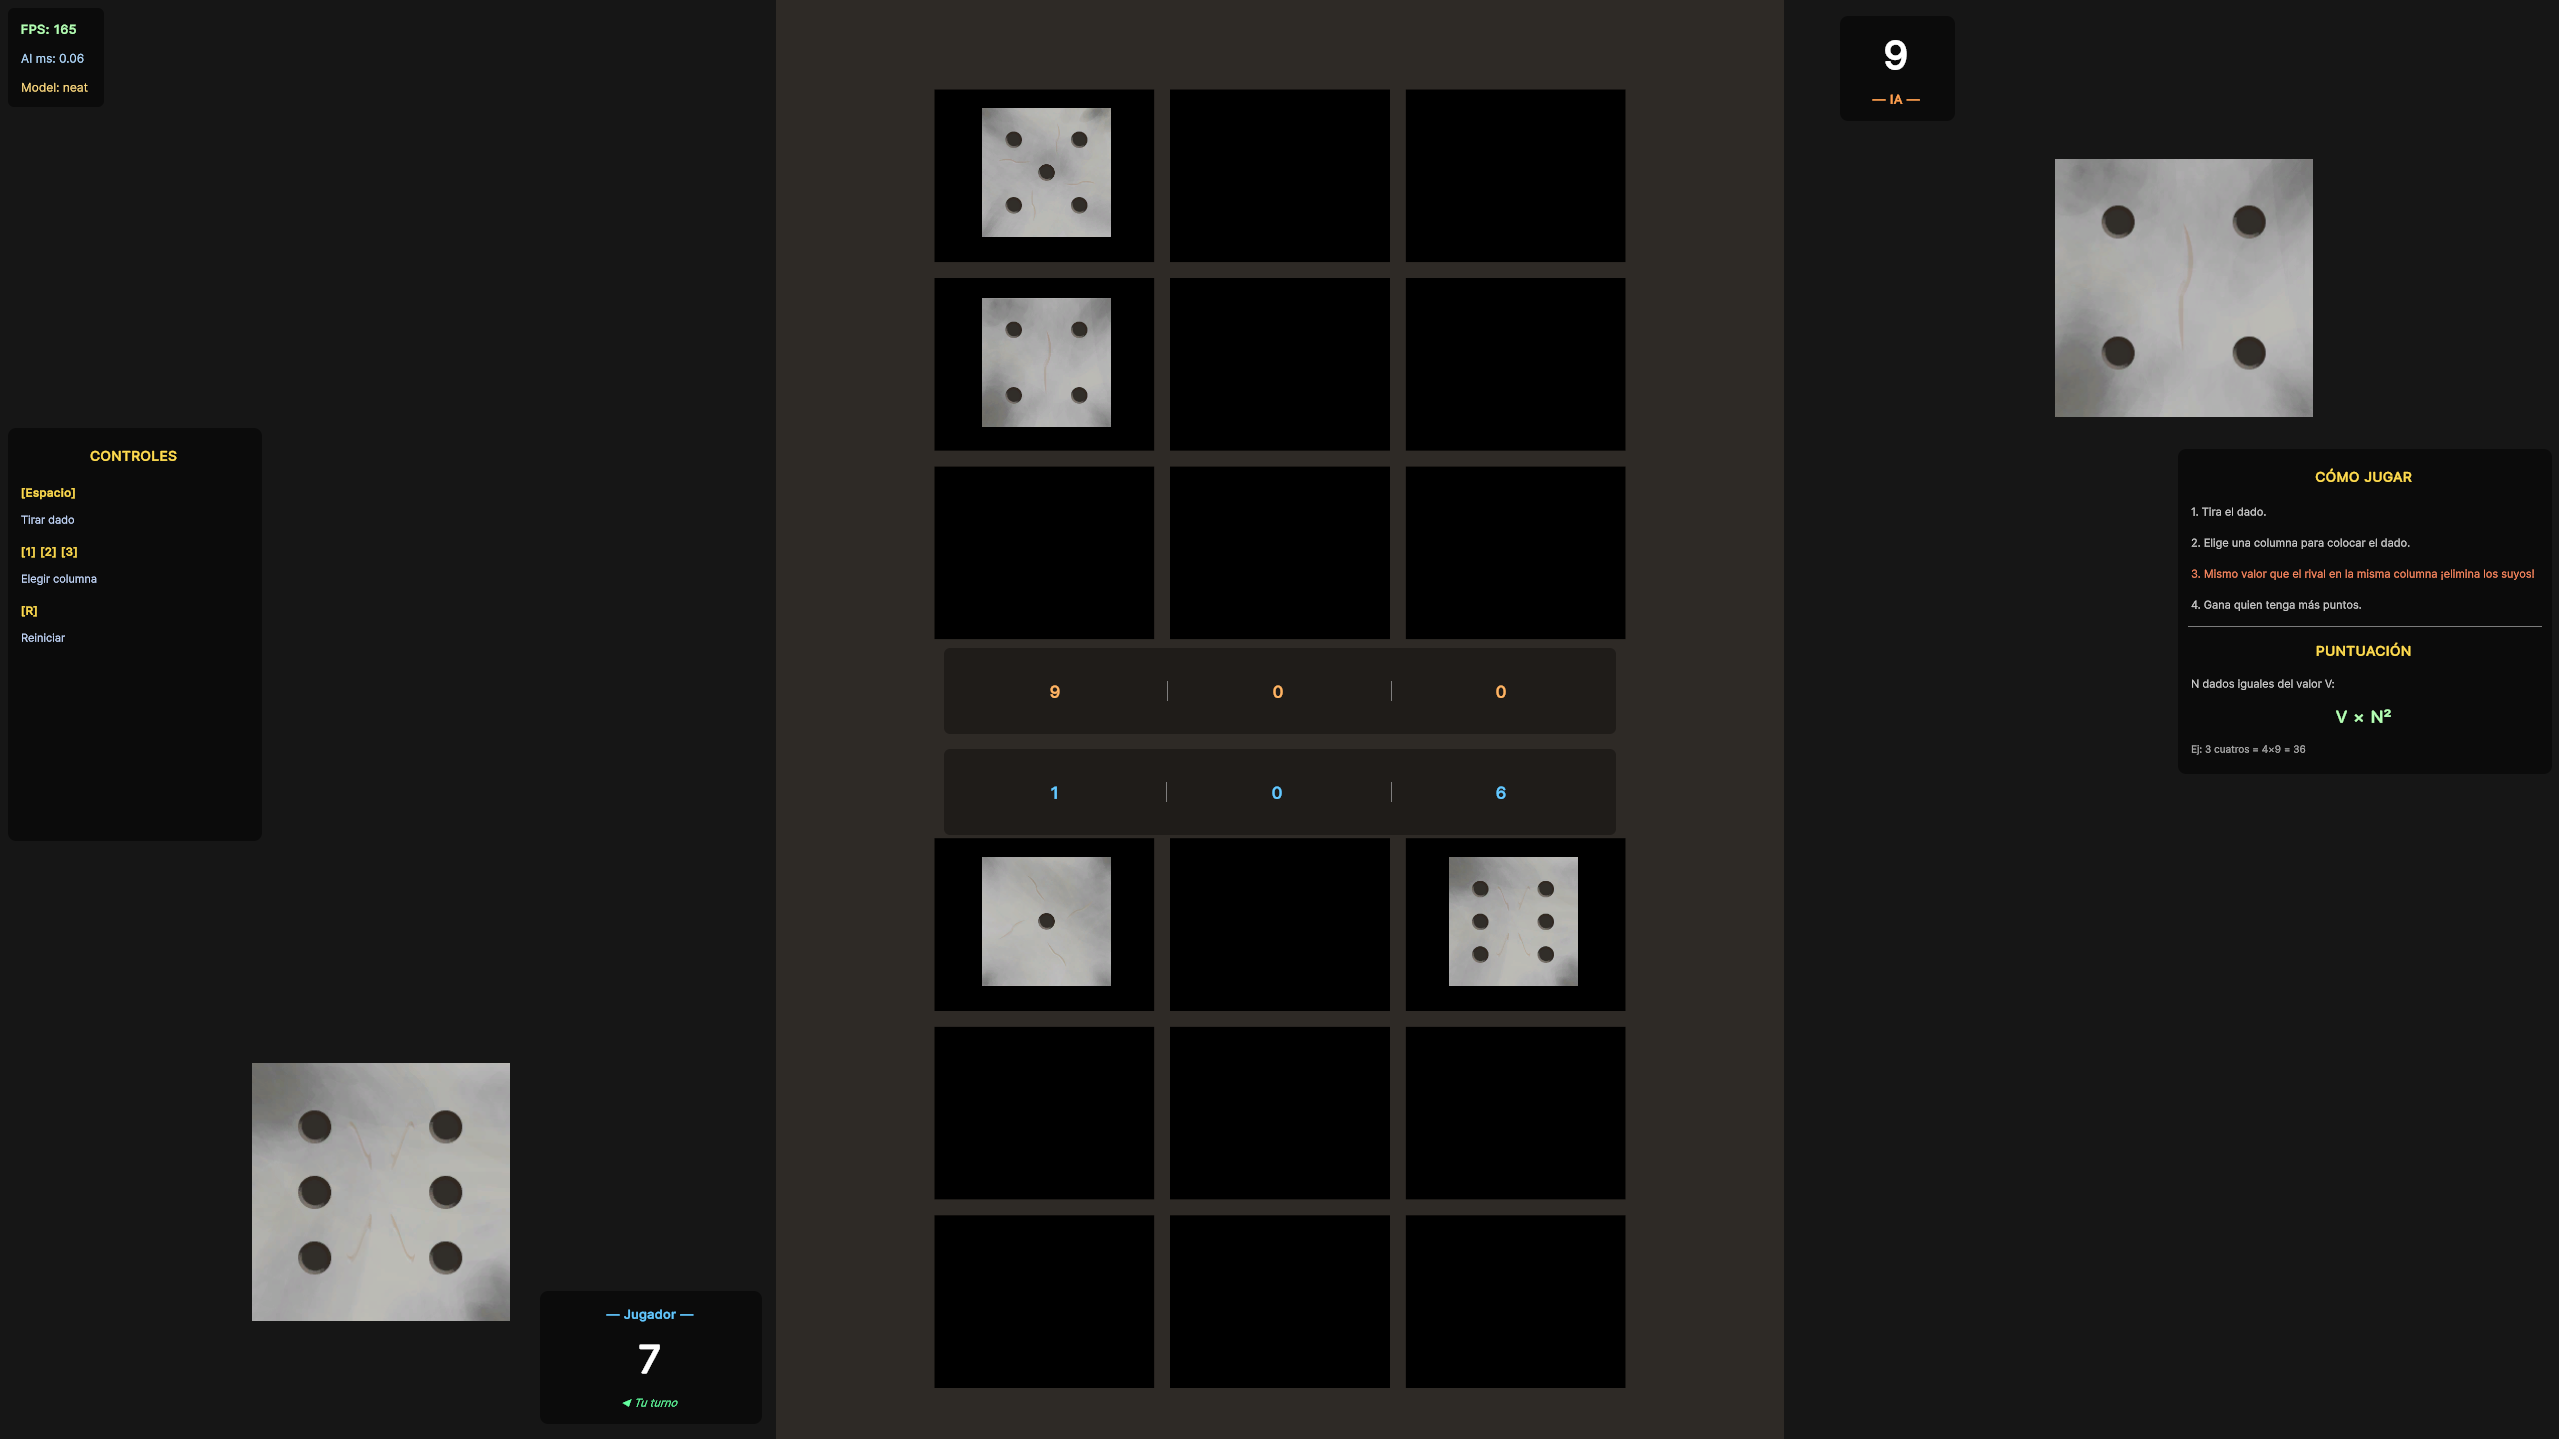
\includegraphics[width=0.85\textwidth]{figures/Knucklebones (3).png}
\caption[Prototipo funcional de Knucklebones en Unity]{Prototipo funcional del juego Knucklebones implementado en Unity con agente de IA externo activo. La interfaz muestra el tablero, el valor del dado actual y las métricas de inferencia utilizadas durante la evaluación del sistema.}
\label{fig:captura_knucklebones}
\end{figure}

\section{Middleware y Comunicación}

La comunicación entre el videojuego y los agentes se realiza mediante un middleware local, utilizando un esquema bloqueante por turno.

El flujo general es:

\begin{enumerate}
    \item El juego emite el estado actual.
    \item El middleware estandariza la representación.
    \item Se extraen características derivadas.
    \item El agente seleccionado retorna una acción.
    \item El middleware registra métricas.
    \item El juego aplica la acción.
\end{enumerate}

Este modelo permite desacoplar completamente la lógica del agente del motor de juego. El flujo de decisión por turno se ilustra en la Figura~\ref{fig:flujo_turno}.

\begin{figure}[H]
\centering
\begin{tikzpicture}[
    flowstep/.style={rectangle, draw, rounded corners, minimum height=0.8cm, minimum width=2.2cm, align=center, font=\footnotesize},
    arrow/.style={-{Stealth[length=2mm]}, thick},
    node distance=0.6cm
]
\node[flowstep, fill=blue!15] (dado) {Tirar dado};
\node[flowstep, fill=blue!15, right=0.5cm of dado] (estado) {Construir\\estado};
\node[flowstep, fill=orange!15, right=0.5cm of estado] (feat) {Extraer\\features (21d)};
\node[flowstep, fill=green!15, right=0.5cm of feat] (agente) {Agente:\\seleccionar\\acción};
\node[flowstep, fill=orange!15, right=0.5cm of agente] (log) {Registrar\\métricas};
\node[flowstep, fill=blue!15, right=0.5cm of log] (aplicar) {Aplicar\\acción};

\draw[arrow] (dado) -- (estado);
\draw[arrow] (estado) -- (feat);
\draw[arrow] (feat) -- (agente);
\draw[arrow] (agente) -- (log);
\draw[arrow] (log) -- (aplicar);

\node[below=0.15cm of dado, font=\tiny\itshape, text=blue!60] {Unity};
\node[below=0.15cm of estado, font=\tiny\itshape, text=blue!60] {Unity};
\node[below=0.15cm of feat, font=\tiny\itshape, text=orange!60] {Middleware};
\node[below=0.15cm of agente, font=\tiny\itshape, text=green!50!black] {Python};
\node[below=0.15cm of log, font=\tiny\itshape, text=orange!60] {Middleware};
\node[below=0.15cm of aplicar, font=\tiny\itshape, text=blue!60] {Unity};
\end{tikzpicture}
\caption[Flujo de decisión por turno]{Flujo de decisión por turno: desde el lanzamiento del dado hasta la aplicación de la acción.}
\label{fig:flujo_turno}
\end{figure}

La Figura~\ref{fig:middleware_real} muestra el middleware en ejecución durante una partida, evidenciando la comunicación activa entre Unity y los agentes Python. Se observa el servidor Flask activo, el sistema cargado y los endpoints expuestos.

\begin{figure}[H]
\centering
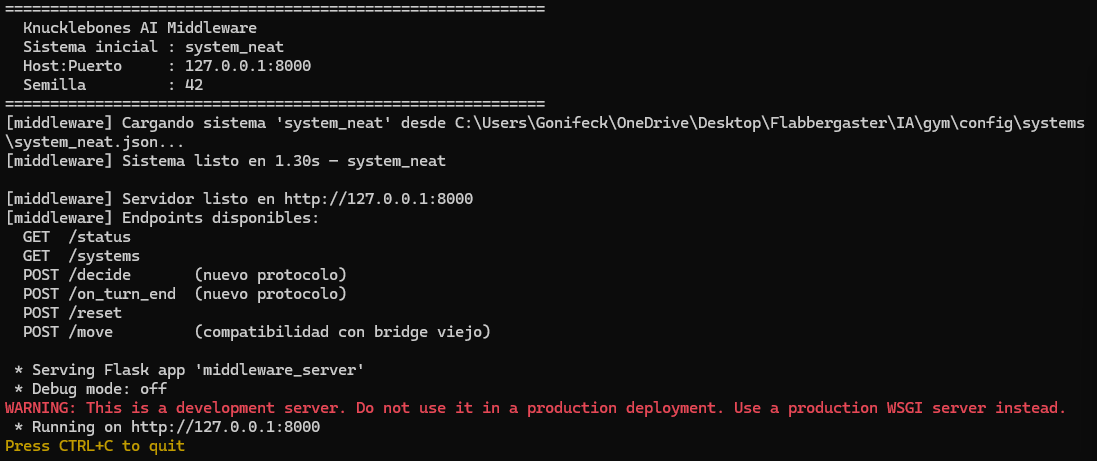
\includegraphics[width=0.75\textwidth]{figures/MiddleWare.png}
\caption[Middleware local en ejecución]{Consola del middleware local en Python. Se observa: (1) el servidor Flask escuchando en el puerto 5000, (2) el sistema adaptativo cargado (system\_neat), y (3) las solicitudes HTTP entrantes desde Unity para los endpoints \texttt{/decide} y \texttt{/status}.}
\label{fig:middleware_real}
\end{figure}

\section{Representación del Estado y Extracción de Características}

Se definió un estado canónico compuesto por:

\begin{itemize}
    \item Tablero propio ($3 \times 3$ valores).
    \item Tablero oponente ($3 \times 3$ valores).
    \item Valor del dado actual.
    \item Puntajes acumulados (propio y rival).
    \item Turno actual.
\end{itemize}

A partir de este estado se calculan 21 características derivadas (features) que alimentan a los agentes de IA. Estas se agrupan en:

\begin{itemize}
    \item \textbf{Características por columna} (3 columnas $\times$ 4 features = 12):
    \begin{itemize}
        \item $ImmediateGain(c)$: incremento de puntaje al colocar el dado en la columna $c$.
        \item $FuturePotential(c)$: potencial de puntuación futura si se completan coincidencias.
        \item $DenialImpact(c)$: reducción del puntaje rival por eliminación de fichas.
        \item $Risk(c)$: exposición a eliminación futura por el rival.
    \end{itemize}
    \item \textbf{Características globales} (9):
    \begin{itemize}
        \item Puntaje propio, puntaje rival, diferencial de puntaje.
        \item Espacios libres por columna (3 valores).
        \item Turno normalizado, ventaja de turno, dado actual normalizado.
    \end{itemize}
\end{itemize}

La centralización del cálculo de características en el middleware evita inconsistencias entre agentes y garantiza que todos operen con la misma representación del estado.

\section{Sistema de Logging e Instrumentación}

Cada turno genera un registro estructurado que incluye:

\begin{itemize}
    \item Estado.
    \item Acción seleccionada.
    \item Agente activo.
    \item Latencia de decisión.
    \item Semilla experimental.
    \item Métricas derivadas.
\end{itemize}

Este registro cumple tres funciones:

\begin{enumerate}
    \item Permitir reconstrucción de partidas.
    \item Construir datasets para entrenamiento supervisado.
    \item Evaluar reproducibilidad experimental.
\end{enumerate}

\section{Control de Aleatoriedad}

Para asegurar comparabilidad entre agentes, se implementó control explícito de semillas (\textit{seed}) para el generador de números aleatorios (RNG).

Esto permite:

\begin{itemize}
    \item Repetir secuencias de juego.
    \item Comparar agentes bajo condiciones idénticas.
    \item Medir estabilidad entre ejecuciones.
\end{itemize}

\section{Entorno de Entrenamiento Equivalente (Gym)}

Debido a restricciones de tiempo y eficiencia de entrenamiento, se desarrolló un entorno equivalente tipo \textit{Gym} que replica las reglas del juego.

Este entorno permite:

\begin{itemize}
    \item Simulación acelerada de partidas.
    \item Generación masiva de datos.
    \item Entrenamiento supervisado o por interacción.
\end{itemize}

El modelo entrenado es posteriormente evaluado bajo el mismo protocolo del entorno principal, garantizando coherencia experimental.

\section{Validación del Simulador Externo}

Dado que el entrenamiento y evaluación de modelos se realiza en un entorno equivalente tipo Gym, fue necesario validar que las reglas implementadas en Python reprodujeran exactamente la lógica del motor Unity.

\subsection{Pruebas de Equivalencia Funcional}

Se generaron trazas de referencia (\textit{golden logs}) desde el entorno Unity, registrando para múltiples turnos:

\begin{itemize}
    \item Estado antes de la acción.
    \item Acción aplicada.
    \item Estado posterior.
    \item Puntajes.
    \item Semilla experimental.
\end{itemize}

Posteriormente, el simulador Python ejecutó la misma secuencia de estados y acciones verificando que:

\[
T_{Unity}(s,a) = T_{Python}(s,a)
\]

para todas las transiciones evaluadas.

La equivalencia exacta de estado posterior garantiza que ambas implementaciones comparten las mismas reglas formales.

\section{Definición Formal de la Política Baseline}

El agente base implementa una política determinista paramétrica basada en combinación ponderada de heurísticas.

Para cada columna disponible $c$ y dado $d$, se calculan:

\begin{itemize}
    \item $ImmediateGain(c,d)$
    \item $FuturePotential(c,d)$
    \item $DenialImpact(c,d)$
    \item $Risk(c,d)$
\end{itemize}

El puntaje compuesto se define como:

\[
ScoreColumn(c,d) =
w_1 ImmediateGain +
w_2 FuturePotential +
w_3 DenialImpact -
w_4 Risk
\]

La acción seleccionada es:

\[
a = \arg\max_c ScoreColumn(c,d)
\]

\subsection{Aleatoriedad Acotada}

Para evitar determinismo absoluto, se introduce un margen relativo $\epsilon$:

\[
\frac{|ScoreColumn(c_i) - ScoreColumn(c_{best})|}{ScoreColumn(c_{best})} < \epsilon
\]

Si múltiples columnas cumplen la condición, se selecciona una aleatoriamente dentro de ese subconjunto.

Esta política constituye el \textit{baseline} contra el cual se comparan los modelos aprendidos.

\subsection{Control de Aleatoriedad}

Para evitar discrepancias en generación de dados, el valor $d$ fue inyectado explícitamente en el simulador durante la validación, eliminando dependencia de generadores RNG internos.

\section{Protocolo Experimental}

Para la evaluación comparativa se definieron:

\subsection{Métricas de desempeño}

\begin{itemize}
    \item Tasa de victoria.
    \item Diferencial de puntaje.
    \item Estabilidad estadística.
\end{itemize}

\subsection{Métricas computacionales}

\begin{itemize}
    \item Latencia promedio de decisión.
    \item Uso de CPU y memoria.
    \item Tiempo de entrenamiento (cuando aplica).
\end{itemize}

Los experimentos se ejecutan con semillas controladas y número fijo de partidas por configuración, permitiendo análisis comparativo reproducible.

\section{Criterios de Viabilidad para Entrenamiento en Tiempo Real}

Un aspecto central de esta investigación es determinar si los paradigmas de aprendizaje evaluados podrían, en principio, ejecutar su proceso de entrenamiento durante una sesión de juego contra un jugador humano, es decir, en tiempo real y en hardware local. Para ello se definen los siguientes criterios de viabilidad, derivados de las condiciones observables en una sesión real de juego.

\subsection{Disponibilidad de datos en una sesión real}

Una partida típica de Knucklebones tiene aproximadamente 18 turnos y dura entre 1 y 3 minutos. Un jugador humano razonablemente comprometido podría jugar entre 10 y 100 partidas antes de perder interés, lo que produce entre 180 y 1,800 muestras de decisión (pares estado-acción). Este volumen se contrasta con los requisitos de entrenamiento de cada paradigma para evaluar la brecha de datos.

\subsection{Requisitos de entrenamiento por paradigma}

\begin{itemize}
    \item \textbf{PPO (Aprendizaje por Refuerzo):} los experimentos utilizaron 400,000 timesteps distribuidos en miles de episodios. Este volumen es varios órdenes de magnitud superior al disponible en una sesión humana.
    \item \textbf{NEAT (Neuroevolución):} el proceso evolutivo requiere evaluar poblaciones completas de genomas durante cientos de generaciones. En la configuración utilizada, cada genoma fue evaluado contra 102 episodios (34 por cada una de 3 semillas), y se mantuvieron poblaciones de 150 genomas durante 300 generaciones, resultando en millones de episodios evaluados en total.
    \item \textbf{DT (Árboles de Decisión destilados):} el entrenamiento supervisado es casi instantáneo ($<$3 segundos), pero depende de un dataset generado por un teacher PPO previamente entrenado. Sin un teacher, no dispone de datos etiquetados.
\end{itemize}

\subsection{Criterio de brecha}

Se define la \textit{brecha de datos} como la relación entre el volumen de datos requerido para obtener un agente funcional y el volumen disponible en una sesión real:

\[
\text{Brecha de datos} = \frac{\text{Datos requeridos para entrenamiento}}{\text{Datos disponibles en sesión real}}
\]

Un valor cercano a 1 indicaría viabilidad; valores de varios órdenes de magnitud indican inviabilidad práctica. Este criterio se evalúa cuantitativamente en el Capítulo~\ref{cap:aplicacion}.

\subsection{Criterio de estabilidad}

Adicionalmente, un modelo que se entrena con datos extremadamente limitados presenta riesgo de:

\begin{itemize}
    \item \textbf{Sobreajuste:} memorizar las pocas partidas observadas en lugar de generalizar.
    \item \textbf{Inestabilidad:} convergencia errática o políticas que varían drásticamente entre ejecuciones.
    \item \textbf{Rendimiento aleatorio:} como se observó en los experimentos con NEAT entrenado con seed fija y pocas generaciones, donde el agente no convergió (WR $\approx$ 0.50, equivalente a aleatorio).
\end{itemize}

Estos criterios permiten evaluar no solo si es posible ejecutar el entrenamiento, sino si el resultado del entrenamiento sería útil bajo las restricciones de una sesión real.



\chapter{Resultados}  \label{cap:aplicacion}
El presente capítulo presenta los resultados experimentales obtenidos al evaluar el rendimiento y desempeño del aprendizaje de tres paradigmas de inteligencia artificial: PPO \cite{schulman2017ppo}, NEAT \cite{stanley2002neat} y Decision Trees destilados \cite{breiman1984classification}. Se analizan, en primer lugar, los costos del proceso de aprendizaje (datos requeridos, tiempo de entrenamiento, recursos computacionales) para evaluar la viabilidad de cada paradigma bajo distintas condiciones de ejecución. En segundo lugar, se presentan las métricas de desempeño de los sistemas adaptativos resultantes. La combinación de ambos análisis permite determinar la factibilidad del aprendizaje en hardware local y la pertinencia de la adaptación por selección de especialistas como alternativa al entrenamiento en tiempo real.

\section{Diseño Experimental}

Los experimentos fueron diseñados con el objetivo de comparar agentes bajo condiciones idénticas, garantizando reproducibilidad y control de variables. El hardware utilizado fue un equipo de escritorio con procesador Intel de 12 núcleos lógicos, GPU NVIDIA GTX 1660 (6 GB VRAM), 16 GB de RAM y sistema operativo Windows 11.

Cada configuración experimental se ejecutó con los siguientes parámetros:

\begin{itemize}
    \item Semilla fija (\texttt{seed=123}) para reproducibilidad.
    \item Número fijo de partidas por evaluación (2,000 a 5,000 según el experimento).
    \item Mismo entorno \texttt{KnucklebonesEnv} como fuente única de verdad.
    \item Registro estructurado por turno y por partida.
\end{itemize}

Los oponentes heurísticos utilizados como benchmark fueron:

\begin{itemize}
    \item \textbf{Greedy}: maximiza el puntaje inmediato.
    \item \textbf{Denial}: prioriza destruir fichas del oponente.
    \item \textbf{Spread}: distribuye fichas entre columnas de forma equilibrada.
\end{itemize}

\section{Entrenamiento de Modelos}

Se entrenaron 10 modelos: 3 PPO, 3 NEAT y 3 DT destilados (uno por cada oponente heurístico), más un perfilador KMeans compartido. La Tabla \ref{tab:training_times} presenta los tiempos de entrenamiento y tamaños resultantes.

\begin{table}[H]
\centering
\caption{Tiempos de entrenamiento y tamaño de modelos}
\begin{tabular}{llrrl}
\hline
\textbf{Familia} & \textbf{Oponente} & \textbf{Tiempo (s)} & \textbf{Tamaño (KB)} & \textbf{Método} \\
\hline
PPO  & denial  & 1,369  & 162 & 4 envs paralelos \\
PPO  & spread  & 390    & 162 & 4 envs paralelos \\
PPO  & greedy  & 400    & 162 & 4 envs paralelos \\
NEAT & denial  & 1,995  & 2.4 & Multi-seed real (3 seeds) \\
NEAT & spread  & 1,868  & 4.2 & Multi-seed real (3 seeds) \\
NEAT & greedy  & 1,818  & 3.6 & Multi-seed real (3 seeds) \\
DT   & denial  & 2.2    & 134 & Behavior Cloning \\
DT   & spread  & 2.0    & 153 & Behavior Cloning \\
DT   & greedy  & 2.0    & 147 & Behavior Cloning \\
KMeans & 4 estilos & 50  & ---  & k=4, ventana=6 \\
\hline
\end{tabular}
\label{tab:training_times}
\end{table}

\textbf{Observaciones clave}:

\begin{itemize}
    \item PPO requirió entre 6 y 23 minutos por especialista (400,000 timesteps) utilizando Stable-Baselines3 \cite{raffin2021sb3} con 4 entornos paralelos (\texttt{SubprocVecEnv}).
    \item NEAT requirió $\sim$30 minutos por especialista (300 generaciones $\times$ 150 genomas $\times$ 102 episodios por genoma con 3 seeds simultáneas, 10 workers paralelos) utilizando neat-python \cite{neatpython2023}. Se adoptó el enfoque multi-seed real para prevenir sobreajuste a secuencias deterministas.
    \item La destilación PPO$\to$DT fue prácticamente instantánea ($<$3 segundos) y redujo el tamaño del modelo $\sim$100$\times$ respecto al PPO original.
    \item KMeans se entrenó en menos de 1 minuto.
    \item Todos los entrenamientos se ejecutaron exclusivamente en CPU, sin requerir GPU.
\end{itemize}

Las Figuras~\ref{fig:training_times} y~\ref{fig:model_sizes} presentan de forma visual la comparativa de tiempos de entrenamiento y tamaños de modelo entre paradigmas.

\begin{figure}[H]
\centering
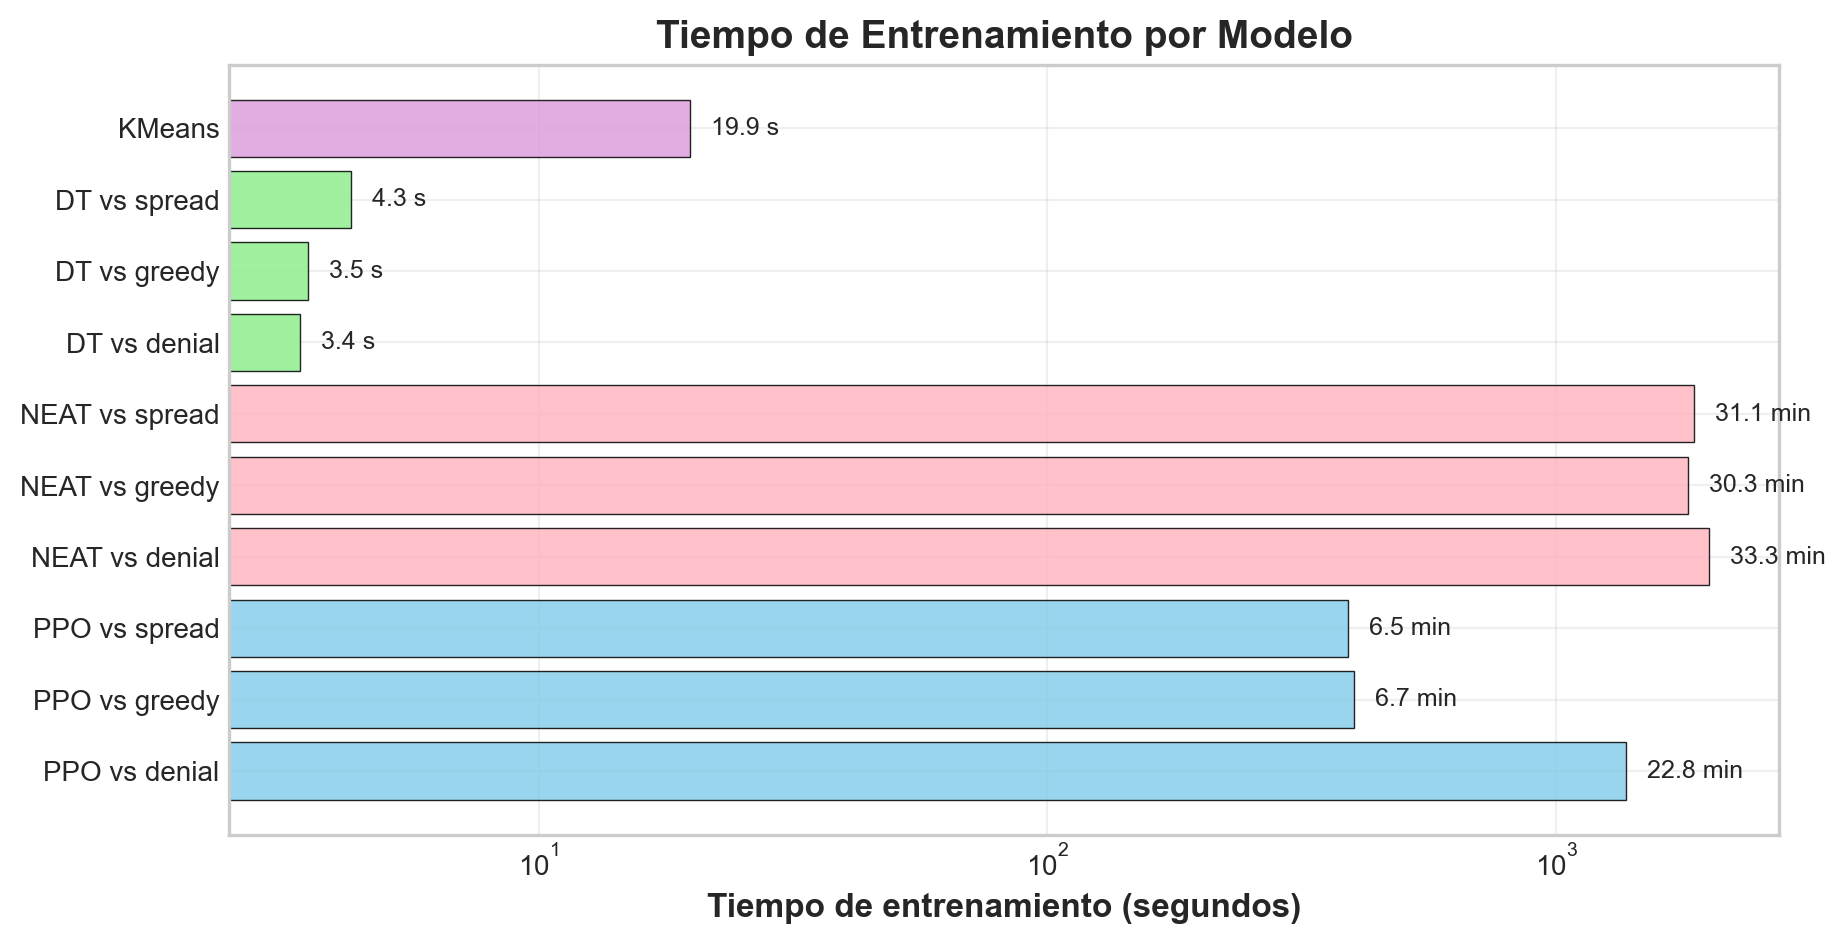
\includegraphics[width=0.75\textwidth]{figures/training_time_comparison.png}
\caption[Tiempos de entrenamiento por paradigma]{Comparativa de tiempos de entrenamiento por paradigma y oponente (escala logarítmica). NEAT requiere $\sim$30 min por especialista; PPO entre 6--23 min; DT $<$3 s por destilación.}
\label{fig:training_times}
\end{figure}

\begin{figure}[H]
\centering
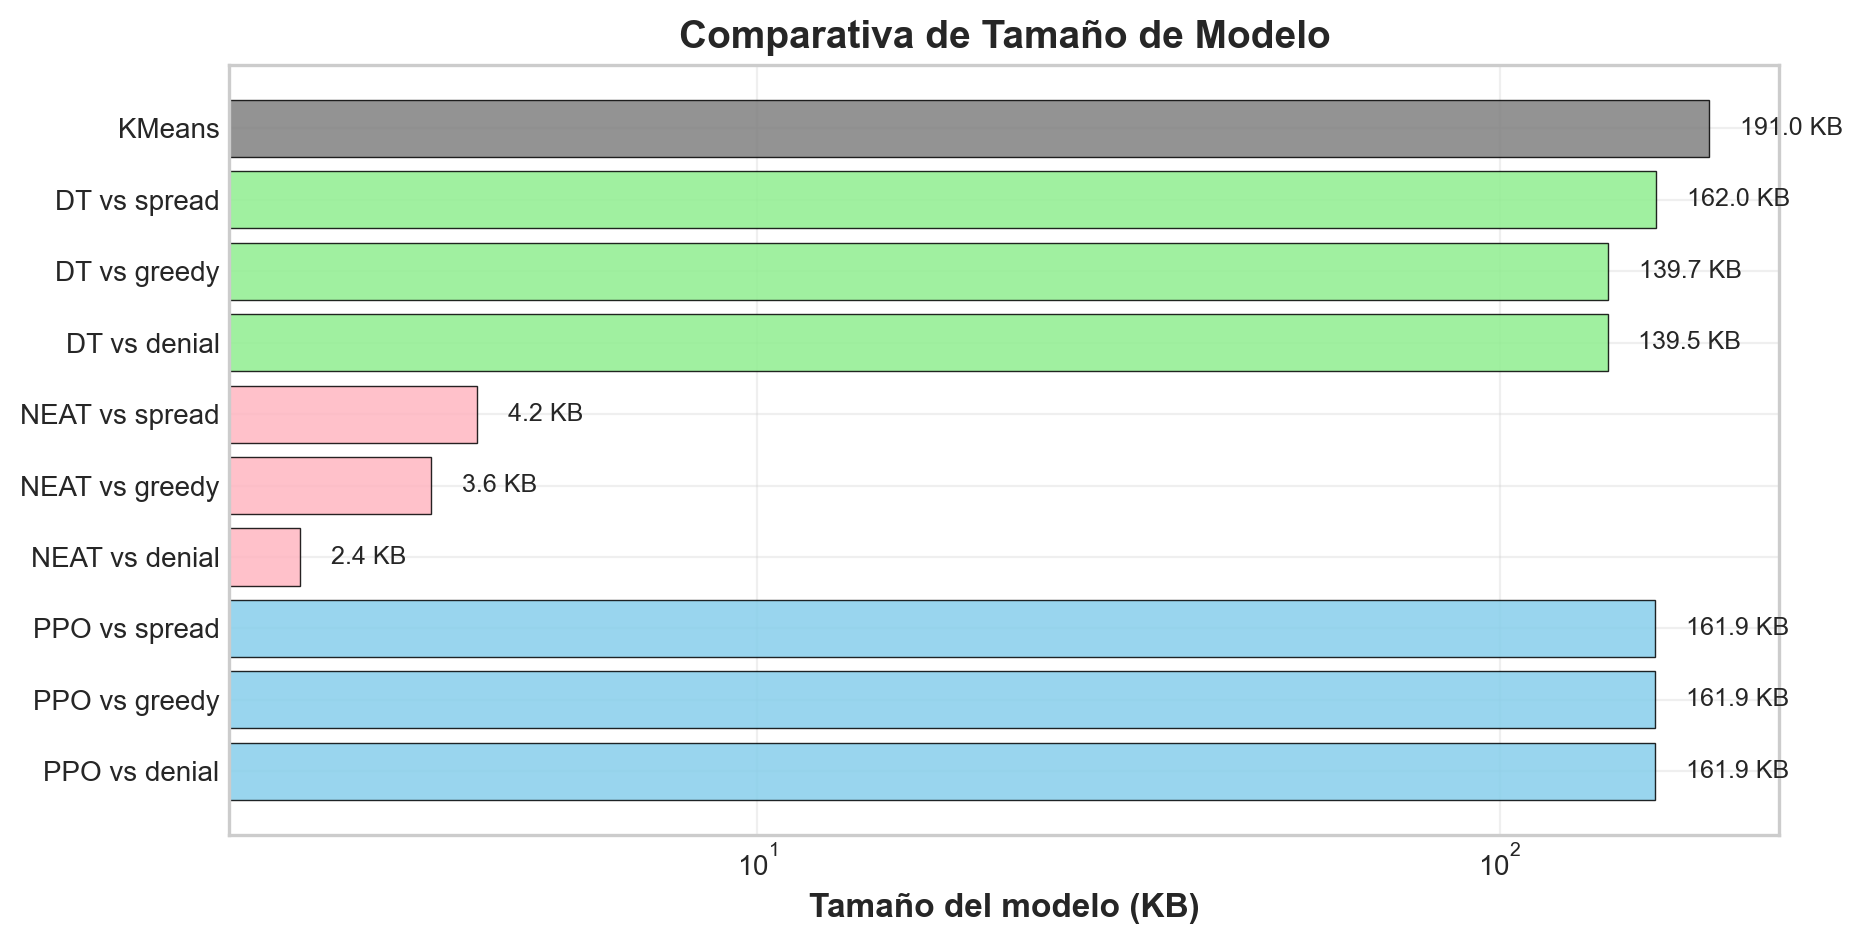
\includegraphics[width=0.75\textwidth]{figures/model_size_comparison.png}
\caption[Tamaño de modelo por paradigma]{Comparativa de tamaño de modelo resultante por paradigma (escala logarítmica). NEAT produce modelos ultraligeros ($\sim$2--4 KB); PPO $\sim$162 KB; DT $\sim$134--153 KB.}
\label{fig:model_sizes}
\end{figure}

\section{Análisis de Brecha: Viabilidad del Aprendizaje en Tiempo Real}

Con los datos de entrenamiento presentados en la Tabla~\ref{tab:training_times}, se evalúa la viabilidad de ejecutar estos mismos procesos de aprendizaje durante una sesión de juego contra un jugador humano.

\subsection{Datos disponibles en una sesión real}

Una partida típica de Knucklebones produce aproximadamente 18 turnos, cada uno generando un par estado-acción utilizable como muestra de entrenamiento. Si se considera que un jugador humano razonablemente comprometido jugaría entre 10 y 100 partidas antes de perder interés, los datos disponibles para entrenamiento durante una sesión real se sitúan entre 180 y 1,800 muestras. La Tabla~\ref{tab:data_gap} presenta la comparación entre estos datos y los requeridos por cada paradigma.

\begin{table}[H]
\centering
\caption{Brecha de datos: requerimiento de entrenamiento vs. disponibilidad en sesión real}
\begin{tabular}{lrrr}
\hline
\textbf{Paradigma} & \textbf{Datos requeridos} & \textbf{Datos en sesión} & \textbf{Factor de brecha} \\
\hline
PPO (400k timesteps)     & $\sim$400,000 samples   & 180--1,800 & $\sim$222--2,222$\times$ \\
NEAT (300 gen $\times$ 150 pop) & $\sim$4,590,000 eps & 180--1,800 & $\sim$2,550--25,500$\times$ \\
DT (Behavior Cloning)    & $\sim$500,000 samples   & 180--1,800 & $\sim$278--2,778$\times$ \\
\hline
\end{tabular}
\label{tab:data_gap}
\end{table}

\subsection{Interpretación de la brecha}

Los tres paradigmas requieren volúmenes de datos entre dos y cuatro órdenes de magnitud superiores a los disponibles en una sesión real. Esta brecha no se resuelve incrementando la velocidad de cómputo, ya que la limitación fundamental es la cantidad de partidas que un jugador humano está dispuesto a jugar. La Figura~\ref{fig:brecha_datos} visualiza esta brecha en escala logarítmica.

\begin{figure}[H]
\centering
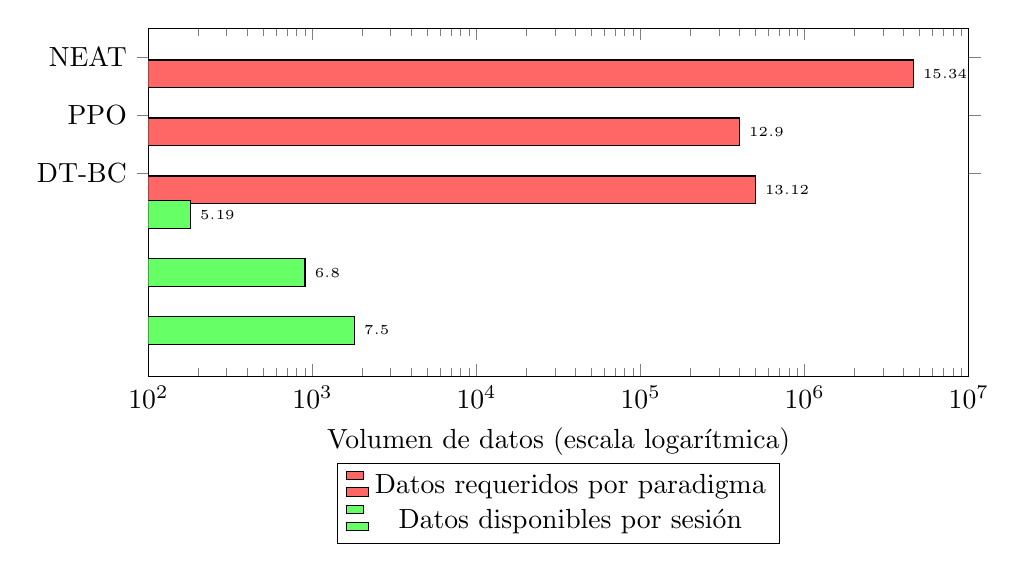
\begin{tikzpicture}
\begin{axis}[
    xbar,
    width=12cm, height=6cm,
    xlabel={Volumen de datos (escala logar\'{i}tmica)},
    symbolic y coords={{Sesi\'{o}n alta (100 part.)}, {Sesi\'{o}n media (50 part.)}, {Sesi\'{o}n baja (10 part.)}, DT-BC, PPO, NEAT},
    ytick=data,
    xmode=log,
    xmin=100, xmax=10000000,
    nodes near coords,
    nodes near coords align={horizontal},
    every node near coord/.append style={font=\tiny},
    bar width=10pt,
    legend style={at={(0.5,-0.25)}, anchor=north},
]
\addplot[fill=red!60] coordinates {(4590000,NEAT) (400000,PPO) (500000,DT-BC)};
\addplot[fill=green!60] coordinates {(1800,{Sesi\'{o}n alta (100 part.)}) (900,{Sesi\'{o}n media (50 part.)}) (180,{Sesi\'{o}n baja (10 part.)})};
\legend{Datos requeridos por paradigma, Datos disponibles por sesi\'{o}n}
\end{axis}
\end{tikzpicture}
\caption[Brecha de datos: entrenamiento vs.\ sesión real]{Brecha de datos entre los requerimientos de entrenamiento de cada paradigma y los datos disponibles en una sesi\'{o}n real contra un jugador humano (escala logar\'{i}tmica). Se observa una diferencia de 2 a 4 \'{o}rdenes de magnitud.}
\label{fig:brecha_datos}
\end{figure}

\subsection{Análisis de sensibilidad}

La estimación de 10--100 partidas por sesión debe interpretarse como un supuesto operativo conservador para el análisis de viabilidad, no como una medición formal de comportamiento de usuarios. Su función es establecer un orden de magnitud razonable para contrastar los requerimientos de entrenamiento. La Tabla~\ref{tab:sensibilidad} presenta tres escenarios que demuestran que la conclusión no cambia dentro de rangos razonables.

\begin{table}[H]
\centering
\caption{Análisis de sensibilidad: brecha de datos bajo tres escenarios de sesión humana}
\begin{tabular}{lccc}
\hline
\textbf{Escenario} & \textbf{Partidas} & \textbf{Muestras ($\sim$18 turnos)} & \textbf{Brecha vs PPO (400k)} \\
\hline
Bajo (pesimista)  & 10  & 180   & $\sim$2,222$\times$ \\
Medio             & 50  & 900   & $\sim$444$\times$ \\
Alto (optimista)  & 100 & 1,800 & $\sim$222$\times$ \\
\hline
\end{tabular}
\label{tab:sensibilidad}
\end{table}

Incluso en el escenario más optimista (100 partidas), la brecha es de más de dos órdenes de magnitud para PPO, el paradigma con menor requerimiento de datos entre los evaluados.

Adicionalmente, los experimentos con NEAT demostraron que el entrenamiento con datos insuficientes produce resultados aleatorios: con seed fija y 100 generaciones, NEAT no convergió (WR $\approx$ 0.50, equivalente a decisiones al azar). Solo cuando se garantizó diversidad y volumen suficiente de episodios (multi-seed real con 102 episodios por genoma) se alcanzó convergencia efectiva (WR = 0.626).

\subsection{Conclusión parcial}

El entrenamiento online continuo durante la partida, en hardware local, no es viable con los paradigmas evaluados debido a la escasez de datos, no solamente por restricciones de tiempo o recursos computacionales. Un jugador humano no genera suficientes muestras de interacción para que cualquiera de los tres enfoques converja a una política funcional.

\section{Calidad de Destilación PPO a DT}

La destilación por \textit{Behavior Cloning} \cite{hussein2017imitation} (aprendizaje supervisado imitando al PPO) produjo árboles de decisión con alta fidelidad al teacher, como se observa en la Tabla \ref{tab:distillation}:

\begin{table}[H]
\centering
\caption{Calidad de destilación: accuracy de los DT respecto al PPO teacher}
\begin{tabular}{lccc}
\hline
\textbf{DT destilado} & \textbf{Accuracy (\%)} & \textbf{Profundidad} & \textbf{Hojas} \\
\hline
dt\_ppo\_vs\_denial  & 93.79 & 10 & 773  \\
dt\_ppo\_vs\_spread  & 93.97 & 10 & 804  \\
dt\_ppo\_vs\_greedy  & 93.85 & 10 & 798  \\
\hline
\end{tabular}
\label{tab:distillation}
\end{table}

La destilación conserva $>$92\% de fidelidad al teacher PPO. Cada DT fue entrenado con $\sim$500,000 muestras generadas en 50,000 episodios de juego del PPO correspondiente.

\section{Perfilado KMeans}

El perfilador KMeans \cite{lloyd1982kmeans} se entrenó con datos de los 4 estilos heurísticos, usando una ventana temporal de 6 turnos. El perfil de cada oponente se representa mediante un vector de 10 dimensiones que captura patrones de decisión:

\begin{itemize}
    \item Histograma de columnas seleccionadas (3 dimensiones).
    \item Histograma de acciones legales disponibles (3 dimensiones).
    \item Proporción de selección de primera/última acción legal (2 dimensiones).
    \item Tasa de repetición de columna (1 dimensión).
    \item Entropía de la distribución de columnas (1 dimensión).
\end{itemize}

Este perfil de 10 dimensiones es independiente de las 21 features usadas por los agentes para seleccionar acciones; su propósito es caracterizar el \textit{estilo de juego} del oponente, no el estado del tablero.

El perfilador se configuró con los siguientes parámetros:

\begin{itemize}
    \item \textbf{k = 4} clusters (uno por cada estilo heurístico).
    \item \textbf{Silhouette score}: 0.232 (separación moderada, esperable dado que los estilos de juego comparten acciones en muchas situaciones).
    \item \textbf{Mapping cluster $\to$ estilo}: Cluster 0 $\to$ greedy, Cluster 1 $\to$ denial, Cluster 2 $\to$ denial, Cluster 3 $\to$ spread.
\end{itemize}

Se observa que 2 de 4 clusters fueron asignados al estilo \textit{denial}, lo que indica que el perfilador tiene dificultades para distinguir completamente entre todos los estilos. Esta limitación se analiza en detalle en la sección de Ablation Study.

\section{Evaluación de los Tres Sistemas Adaptativos}

Cada sistema adaptativo combina el perfilador KMeans compartido con una response table y tres especialistas de su paradigma. Se evaluaron los 3 sistemas contra los 3 oponentes heurísticos (5,000 partidas por matchup). Los resultados se presentan en la Tabla \ref{tab:systems_comparison}.

\begin{table}[H]
\centering
\caption{Winrate decidido de cada sistema vs cada oponente (5,000 partidas)}
\begin{tabular}{lcccc}
\hline
\textbf{Sistema} & \textbf{vs denial} & \textbf{vs spread} & \textbf{vs greedy} & \textbf{Promedio} \\
\hline
System NEAT & \textbf{0.635} & \textbf{0.697} & \textbf{0.626} & \textbf{0.653} \\
System DT   & 0.592          & 0.641          & 0.591          & 0.608 \\
System PPO  & 0.588          & 0.641          & 0.584          & 0.604 \\
\hline
\end{tabular}
\label{tab:systems_comparison}
\end{table}

El sistema NEAT alcanza un winrate promedio de 0.653 (IC 95\%: [0.645, 0.660]), significativamente superior a DT (0.608, IC: [0.600, 0.616]) y PPO (0.604, IC: [0.597, 0.612]). Este resultado se obtuvo tras implementar el entrenamiento multi-seed real, que mejoró la convergencia de NEAT.

\subsection{Resultados detallados por sistema}

A continuación se presentan los resultados desglosados de cada sistema adaptativo por oponente heurístico. Cada tabla muestra el número de partidas evaluadas, el winrate decidido (excluyendo empates), el intervalo de confianza al 95\%, el diferencial promedio de puntaje y el tiempo de ejecución.

\begin{table}[H]
\centering
\caption{System DT --- KMeans + Decision Trees destilados de PPO}
\begin{tabular}{lrccrc}
\hline
\textbf{Oponente} & \textbf{Games} & \textbf{WR decidido} & \textbf{IC 95\%} & \textbf{Avg diff} & \textbf{Wall (s)} \\
\hline
denial & 5,000 & 0.592 & [0.578, 0.606] & +4.80 & 30.4 \\
spread & 5,000 & 0.641 & [0.628, 0.654] & +8.06 & 40.0 \\
greedy & 5,000 & 0.591 & [0.577, 0.605] & +4.68 & 28.5 \\
\hline
\end{tabular}
\label{tab:system_dt}
\end{table}

\begin{table}[H]
\centering
\caption{System PPO --- KMeans + PPO especialistas directos}
\begin{tabular}{lrccrc}
\hline
\textbf{Oponente} & \textbf{Games} & \textbf{WR decidido} & \textbf{IC 95\%} & \textbf{Avg diff} & \textbf{Wall (s)} \\
\hline
denial & 5,000 & 0.588 & [0.574, 0.602] & +4.70 & 45.2 \\
spread & 5,000 & 0.641 & [0.628, 0.655] & +8.00 & 44.3 \\
greedy & 5,000 & 0.584 & [0.571, 0.598] & +4.50 & 43.1 \\
\hline
\end{tabular}
\label{tab:system_ppo}
\end{table}

\begin{table}[H]
\centering
\caption{System NEAT --- KMeans + NEAT especialistas directos (multi-seed)}
\begin{tabular}{lrccrc}
\hline
\textbf{Oponente} & \textbf{Games} & \textbf{WR decidido} & \textbf{IC 95\%} & \textbf{Avg diff} & \textbf{Wall (s)} \\
\hline
denial & 5,000 & 0.635 & [0.621, 0.648] & +6.40 & 28.8 \\
spread & 5,000 & 0.697 & [0.684, 0.710] & +11.0 & 27.4 \\
greedy & 5,000 & 0.626 & [0.613, 0.640] & +6.00 & 27.1 \\
\hline
\end{tabular}
\label{tab:system_neat}
\end{table}

\section{Análisis Estadístico entre Sistemas}

Se aplicó un \textbf{z-test de dos proporciones} (bilateral) a cada par de sistemas por oponente (9 comparaciones), con corrección de Bonferroni para comparaciones múltiples. Los valores $p$ se presentan en la Tabla \ref{tab:ztest}.

\begin{table}[H]
\centering
\caption{Valores p del z-test entre pares de sistemas (corregidos por Bonferroni)}
\begin{tabular}{lccc}
\hline
\textbf{Par comparado} & \textbf{vs denial ($p$)} & \textbf{vs spread ($p$)} & \textbf{vs greedy ($p$)} \\
\hline
DT vs PPO   & 1.000 & 1.000 & 1.000 \\
DT vs NEAT  & \textbf{0.0001} & \textbf{$<$0.0001} & \textbf{0.003} \\
PPO vs NEAT & \textbf{$<$0.0001} & \textbf{$<$0.0001} & \textbf{0.0002} \\
\hline
\end{tabular}
\label{tab:ztest}
\end{table}

\textbf{Resultado}: 6 de 9 comparaciones son estadísticamente significativas tras corrección de Bonferroni ($\alpha = 0.05$). El sistema NEAT es significativamente superior tanto a DT como a PPO en los tres oponentes evaluados. No se observa diferencia significativa entre DT y PPO. Las Figuras~\ref{fig:score_diff_dt}, \ref{fig:score_diff_ppo} y \ref{fig:score_diff_neat} muestran la distribución de los diferenciales de puntaje por paradigma, y la Figura~\ref{fig:score_diff_consolidated} presenta la comparativa consolidada de los sistemas adaptativos.

\begin{figure}[H]
\centering
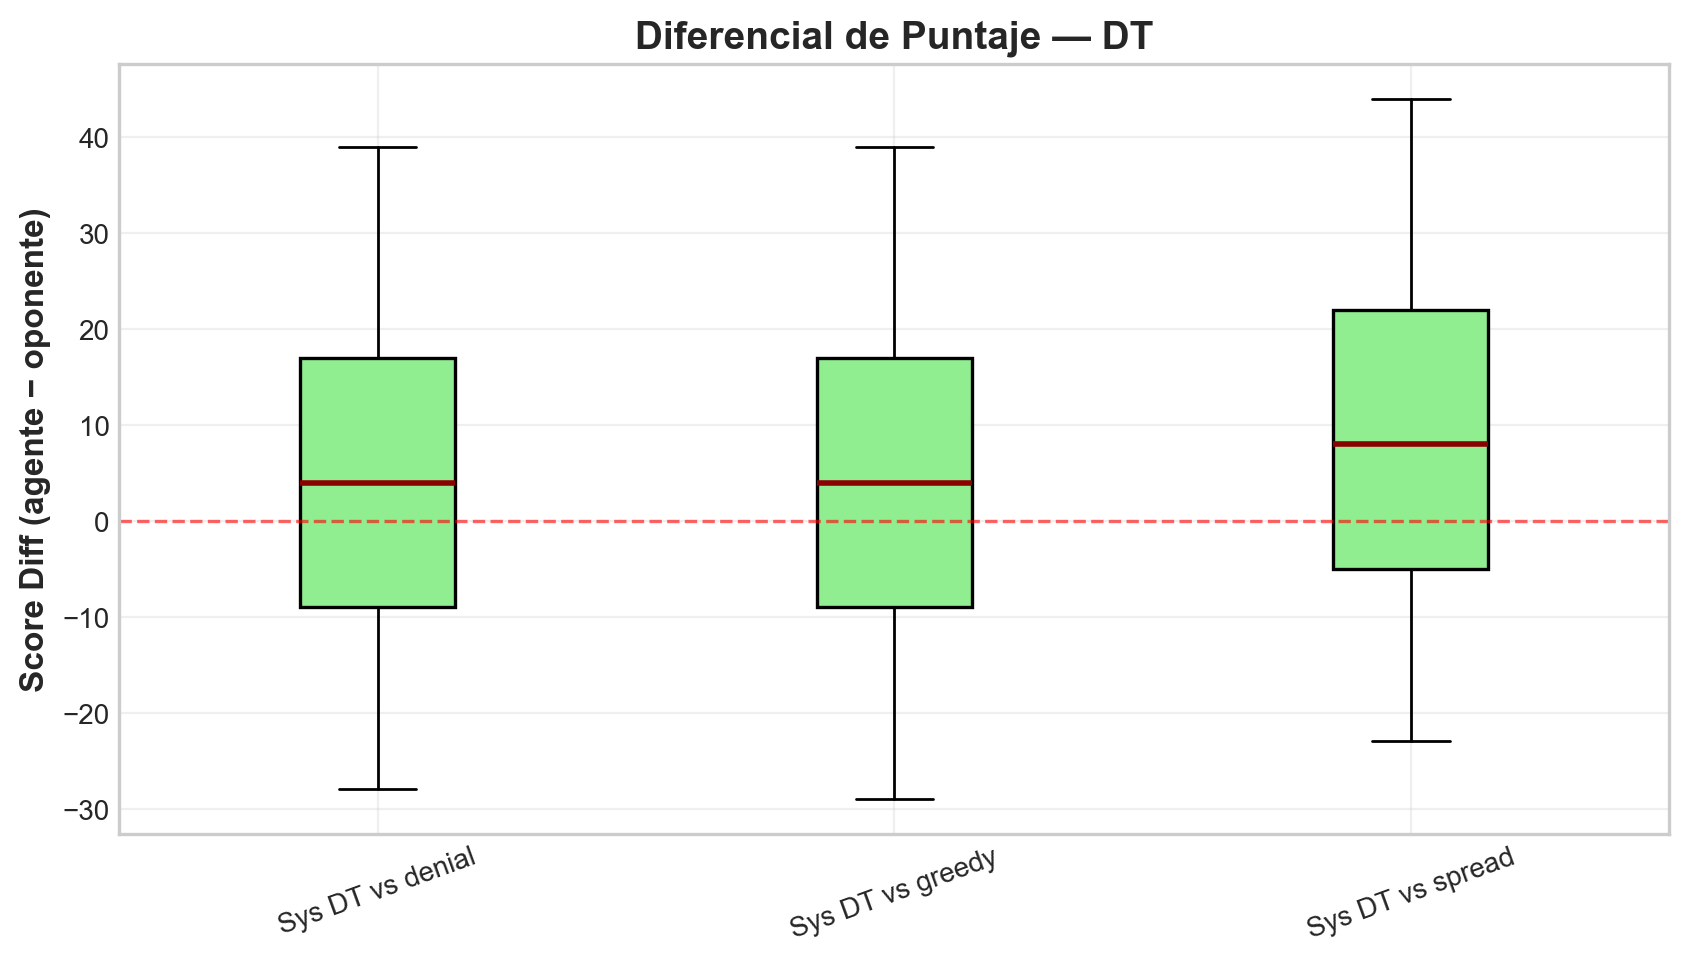
\includegraphics[width=0.85\textwidth]{figures/score_diff_dt.png}
\caption[Diferencial de puntaje --- DT]{Diferencial de puntaje para el paradigma DT (Decision Trees destilados). Las cajas representan percentiles p25--p75 y los bigotes p5--p95.}
\label{fig:score_diff_dt}
\end{figure}

\begin{figure}[H]
\centering
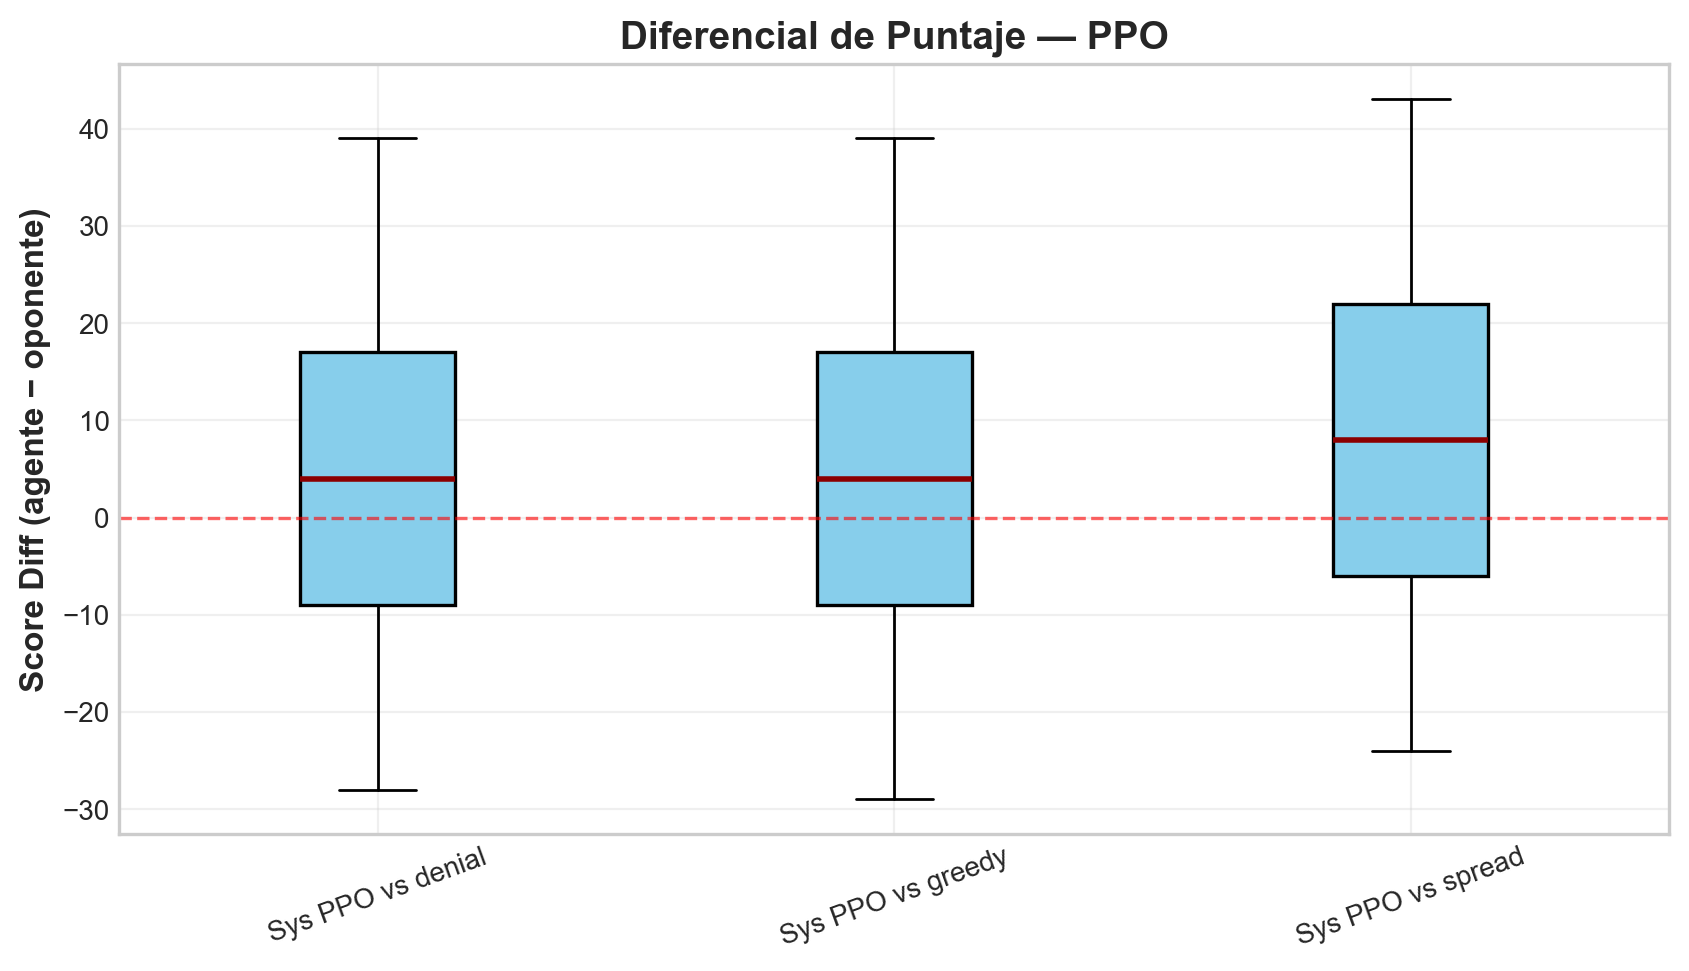
\includegraphics[width=0.85\textwidth]{figures/score_diff_ppo.png}
\caption[Diferencial de puntaje --- PPO]{Diferencial de puntaje para el paradigma PPO (Proximal Policy Optimization).}
\label{fig:score_diff_ppo}
\end{figure}

\begin{figure}[H]
\centering
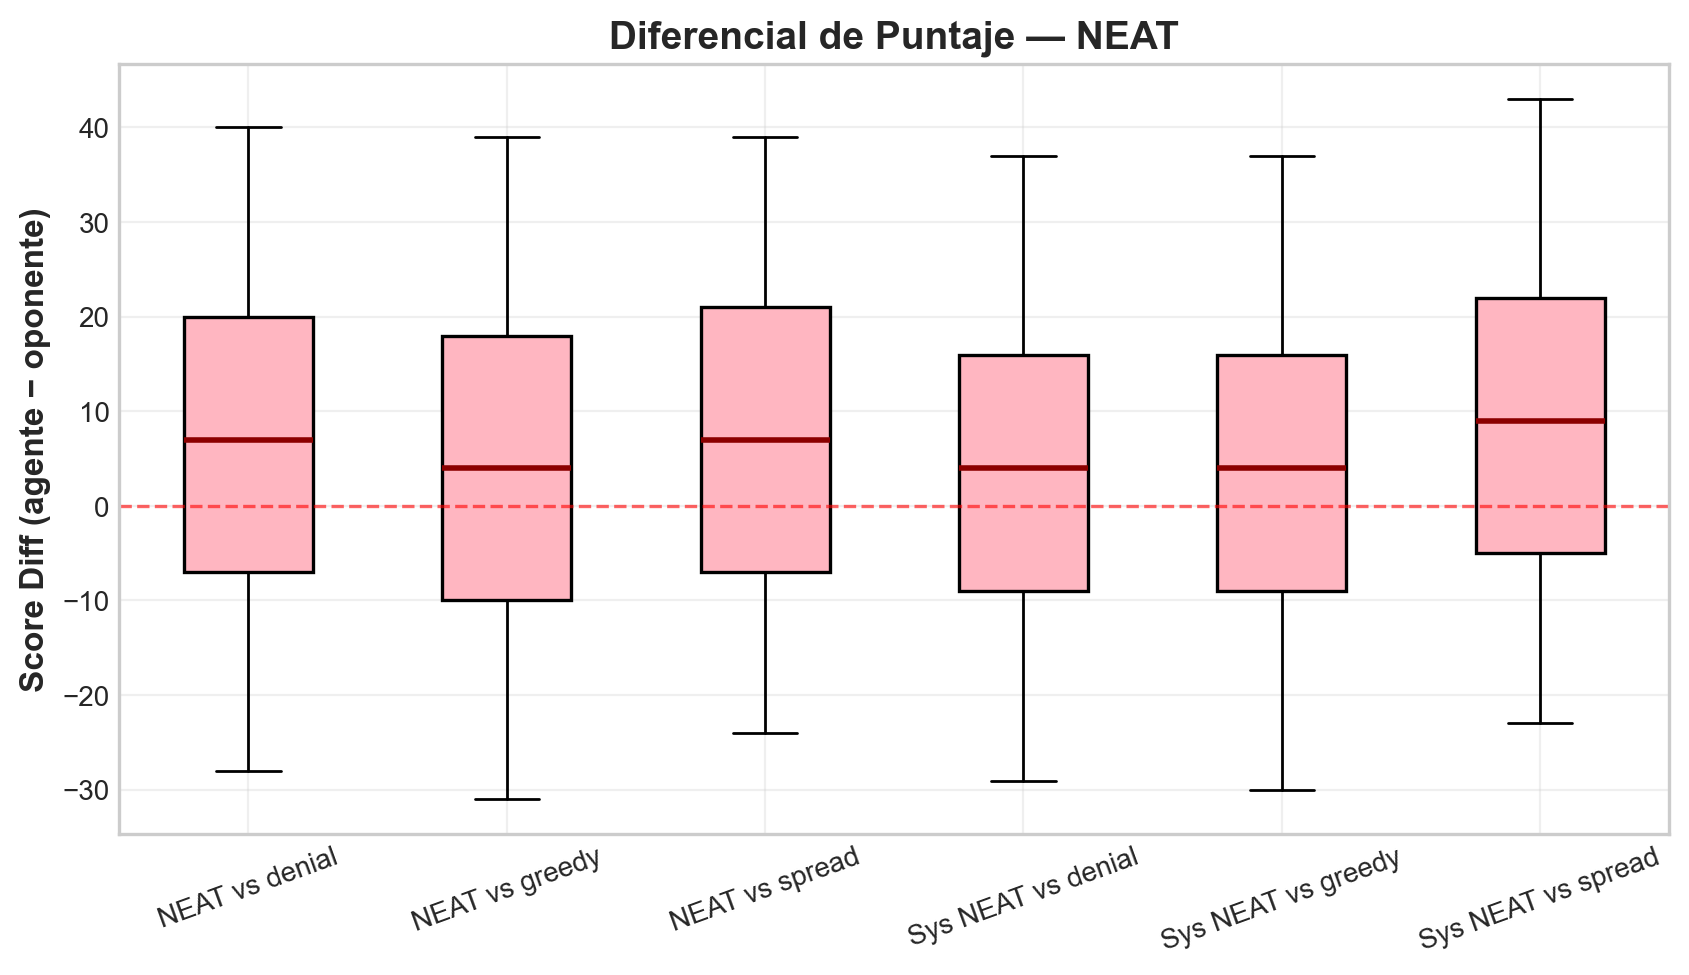
\includegraphics[width=0.85\textwidth]{figures/score_diff_neat.png}
\caption[Diferencial de puntaje --- NEAT]{Diferencial de puntaje para el paradigma NEAT (NeuroEvolution of Augmenting Topologies).}
\label{fig:score_diff_neat}
\end{figure}

\begin{figure}[H]
\centering
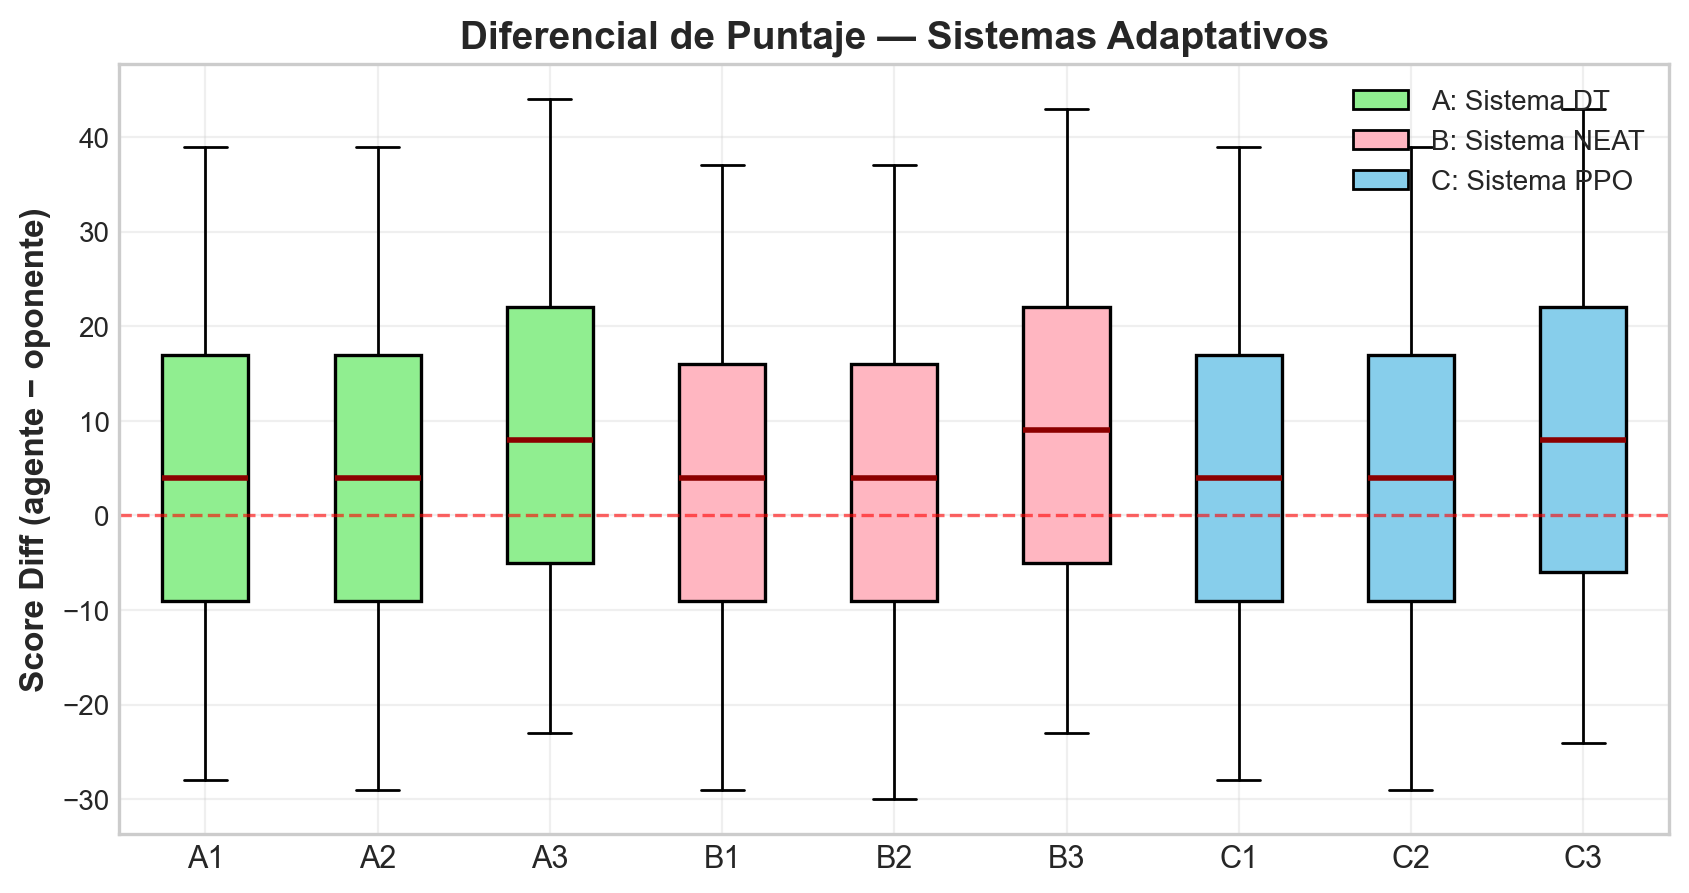
\includegraphics[width=0.9\textwidth]{figures/score_diff_boxplot.png}
\caption[Diferencial de puntaje --- Sistemas adaptativos]{Comparativa consolidada del diferencial de puntaje de los tres sistemas adaptativos. Variables: A = Sistema DT, B = Sistema NEAT, C = Sistema PPO. Subíndices: 1 = vs denial, 2 = vs greedy, 3 = vs spread. El sistema NEAT (rosa) muestra mayor ventaja promedio.}
\label{fig:score_diff_consolidated}
\end{figure}

\section{Ablation Study: ¿Aporta la Adaptación KMeans?}

Para cada familia se compararon cuatro condiciones, como se muestra en la Tabla \ref{tab:ablation}:

\begin{table}[H]
\centering
\caption{Ablation study: generalista vs adaptativo vs oráculo}
\begin{tabular}{lcccc}
\hline
\textbf{Familia} & \textbf{Peor gen.} & \textbf{Mejor gen.} & \textbf{Sistema adapt.} & \textbf{$\Delta$ Sist. vs Mejor} \\
\hline
DT   & 0.585 & 0.618 & 0.608 & $-$0.010 \\
PPO  & 0.572 & 0.610 & 0.604 & $-$0.005 \\
NEAT & 0.543 & \textbf{0.651} & \textbf{0.653} & +0.002  \\
\hline
\end{tabular}
\label{tab:ablation}
\end{table}

\textbf{Hallazgo clave}: el sistema adaptativo \textbf{no mejora} sobre el mejor generalista fijo en DT ($-$0.010 WR) y PPO ($-$0.005 WR). En NEAT muestra una mejora marginal (+0.002). Este resultado, lejos de invalidar el mecanismo de adaptación, lo posiciona como una alternativa operativamente viable: el mecanismo adaptativo es arquitectónicamente válido y mantiene rendimiento competitivo comparable al mejor generalista fijo, sin reentrenamiento en runtime y con costo computacional de inferencia despreciable (microsegundos). En Knucklebones, la baja diversidad estratégica del dominio limita el beneficio de la selección adaptativa; en juegos con mayor variedad de estilos de oponente se esperaría un beneficio más pronunciado.

La brecha de datos documentada en la sección anterior demuestra que el entrenamiento online no es una opción viable. La adaptación por selección cierra esta brecha al trasladar el costo del aprendizaje a la fase offline, manteniendo la capacidad de respuesta diferenciada en tiempo de ejecución.

\begin{enumerate}
    \item El KMeans asigna 2 de 4 clusters al estilo \textit{denial}, reduciendo su capacidad discriminante.
    \item Un solo especialista (entrenado vs greedy) resulta fuerte contra todos los oponentes.
    \item La response table ocasionalmente selecciona un especialista subóptimo para un cluster.
\end{enumerate}

\subsection{Dominancia en Response Tables}

La Tabla \ref{tab:dominance} muestra qué especialista fue seleccionado con mayor frecuencia por cada response table.

\begin{table}[H]
\centering
\caption{Dominancia de especialistas en las response tables}
\begin{tabular}{lcc}
\hline
\textbf{Sistema} & \textbf{Especialista dominante} & \textbf{Cobertura} \\
\hline
System DT   & dt\_vs\_denial    & 2/4 (50\%)  \\
System PPO  & PPO\_vs\_denial        & 2/4 (50\%)  \\
System NEAT & neat\_vs\_denial       & 4/4 (100\%) \\
\hline
\end{tabular}
\label{tab:dominance}
\end{table}

\textbf{Interpretación}: el mecanismo adaptativo es arquitectónicamente válido, pero en Knucklebones los estilos no son suficientemente distintos para que la selección diferenciada aporte mejora competitiva significativa. En DT y PPO se utilizan 3 especialistas distintos (uno por estilo dominante en cada cluster), mientras que en NEAT un solo especialista (denial) domina todos los clusters, indicando que aprendió una política generalista fuerte. En juegos con mayor diversidad estratégica se esperaría una distribución más equilibrada entre especialistas.

\textit{Nota}: los datos de esta tabla fueron extraídos directamente de los archivos de response table generados por \texttt{build\_response\_table.py}, los cuales registran la selección óptima de especialista por cluster según winrate decidido.

\section{Evaluación Cruzada: Generalización vs Sobreajuste}

Cada especialista se evaluó contra \textbf{todos} los oponentes (2,000 partidas por matchup) para detectar sobreajuste. El símbolo $\star$ indica el oponente contra el que fue entrenado. Los resultados por familia se presentan en las Tablas \ref{tab:cross_neat}, \ref{tab:cross_ppo} y \ref{tab:cross_dt}, con un resumen de generalización en la Tabla \ref{tab:generalization}.

\begin{table}[H]
\centering
\caption{Evaluación cruzada de NEAT especialistas (winrate decidido)}
\begin{tabular}{lccc}
\hline
\textbf{Especialista} & \textbf{vs denial} & \textbf{vs spread} & \textbf{vs greedy} \\
\hline
NEAT $\to$ denial & 0.635$\star$ & 0.692 & 0.627 \\
NEAT $\to$ spread & 0.496 & 0.634$\star$ & 0.499 \\
NEAT $\to$ greedy & 0.635 & 0.692 & 0.627$\star$ \\
\hline
\end{tabular}
\label{tab:cross_neat}
\end{table}

Se observa que los especialistas NEAT entrenados contra denial y greedy convergen a políticas similares, ambas generalistas fuertes (WR $>$ 0.62 contra todos los oponentes). En contraste, el especialista entrenado contra spread presenta bajo rendimiento generalista.

\begin{table}[H]
\centering
\caption{Evaluación cruzada de PPO especialistas (winrate decidido)}
\begin{tabular}{lccc}
\hline
\textbf{Especialista} & \textbf{vs denial} & \textbf{vs spread} & \textbf{vs greedy} \\
\hline
PPO $\to$ denial & 0.598$\star$ & 0.625 & 0.589 \\
PPO $\to$ spread & 0.531 & 0.650$\star$ & 0.535 \\
PPO $\to$ greedy & 0.600 & 0.626 & 0.602$\star$ \\
\hline
\end{tabular}
\label{tab:cross_ppo}
\end{table}

Los especialistas PPO muestran un patrón similar: el entrenado contra greedy es el mejor generalista, mientras que el de spread es el más especializado.

\begin{table}[H]
\centering
\caption{Evaluación cruzada de DT especialistas (winrate decidido)}
\begin{tabular}{lccc}
\hline
\textbf{Especialista} & \textbf{vs denial} & \textbf{vs spread} & \textbf{vs greedy} \\
\hline
DT $\to$ denial & 0.589$\star$ & 0.633 & 0.589 \\
DT $\to$ spread & 0.549 & 0.656$\star$ & 0.548 \\
DT $\to$ greedy & 0.601 & 0.651 & 0.601$\star$ \\
\hline
\end{tabular}
\label{tab:cross_dt}
\end{table}

Los DT destilados heredan el comportamiento de sus teachers PPO, mostrando patrones de generalización similares. La Tabla~\ref{tab:generalization} resume los resultados de generalización de las tres familias.

\begin{table}[H]
\centering
\caption{Resumen de generalización por familia}
\begin{tabular}{lcc}
\hline
\textbf{Familia} & \textbf{$\Delta$ promedio} & \textbf{Veredicto} \\
\hline
NEAT & +0.007 & Sin sobreajuste \\
PPO  & +0.018 & Sin sobreajuste \\
DT   & +0.010 & Sin sobreajuste \\
\hline
\end{tabular}
\label{tab:generalization}
\end{table}

\textbf{Hallazgos}:

\begin{enumerate}
    \item No se detecta sobreajuste ($\Delta < 3\%$ en todas las familias).
    \item Spread es el oponente más ``fácil'' ($\sim$0.63--0.69 independientemente del entrenamiento).
    \item NEAT\_vs\_denial y NEAT\_vs\_greedy convergen a políticas generalistas fuertes con multi-seed (WR $>$ 0.62 contra todo).
    \item NEAT\_vs\_spread sigue siendo el más débil, mostrando que el estilo de entrenamiento importa.
    \item Los especialistas entrenados contra greedy son los mejores generalistas en PPO y DT.
\end{enumerate}

La Figura~\ref{fig:cross_eval_heatmap} presenta visualmente los resultados de la evaluación cruzada mediante un mapa de calor, donde se observa claramente que los especialistas entrenados contra spread tienen menor capacidad de generalización.

\begin{figure}[H]
\centering
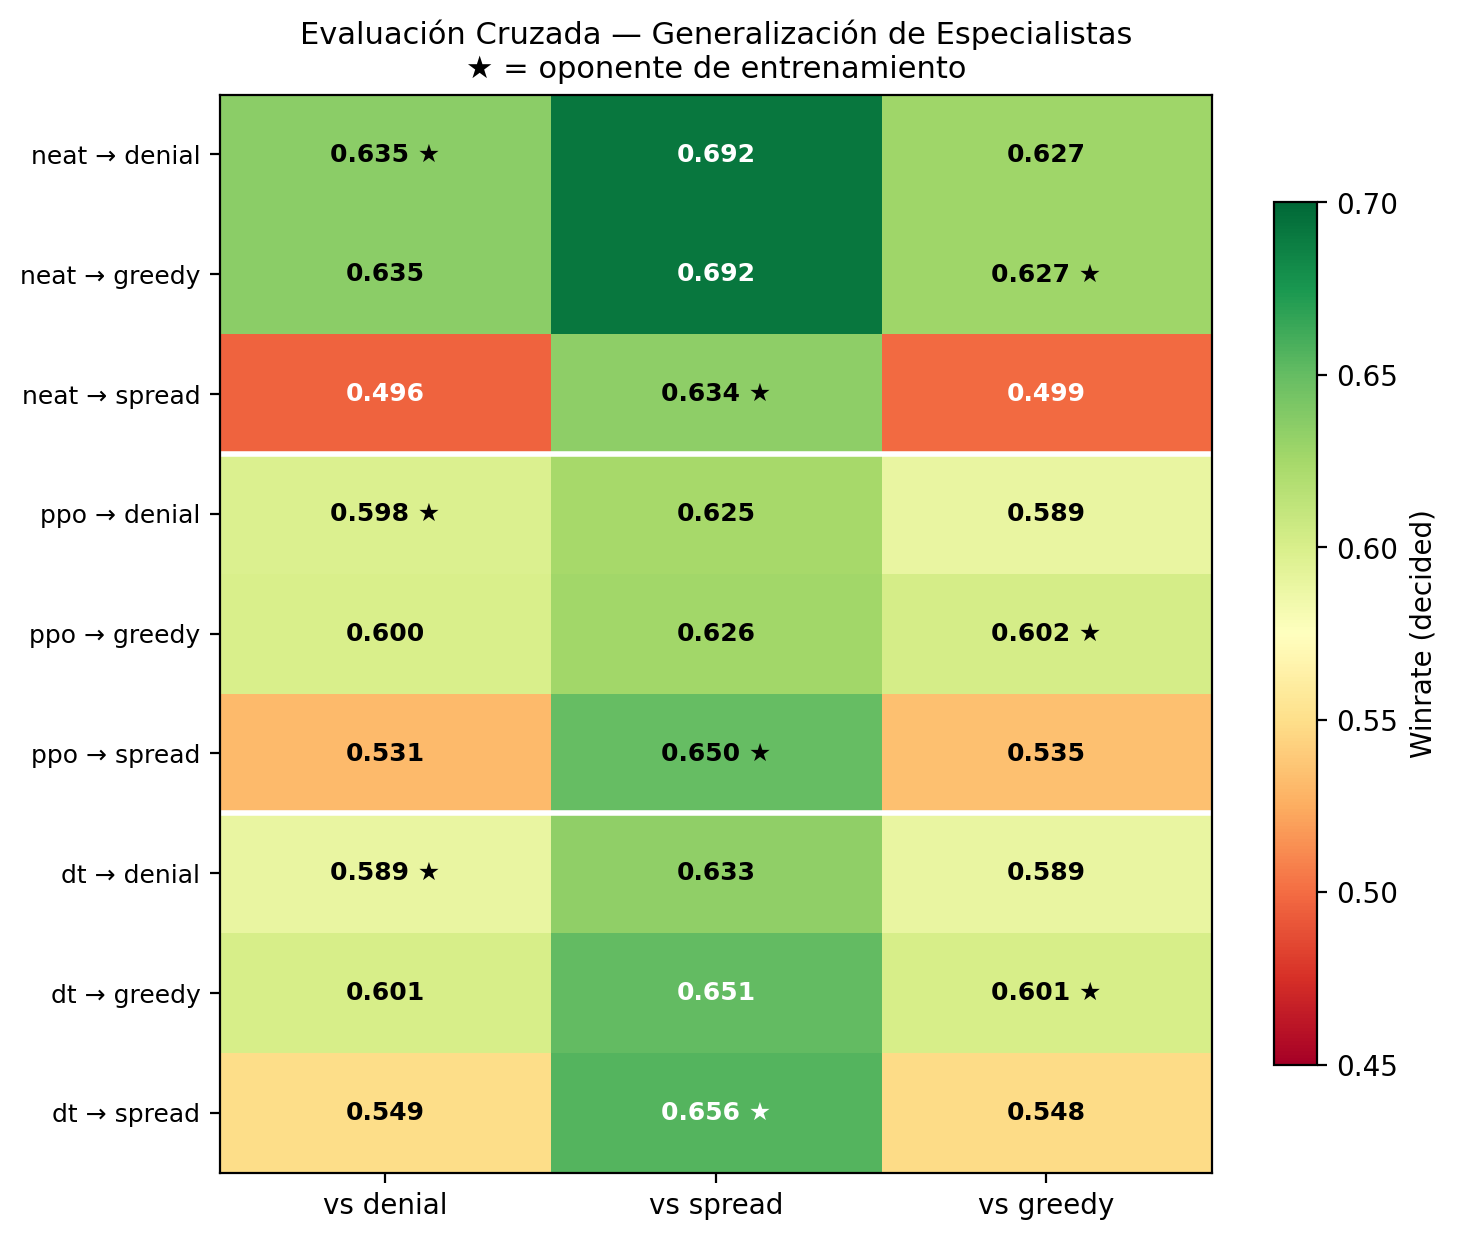
\includegraphics[width=0.85\textwidth]{figures/cross_eval_heatmap.png}
\caption[Mapa de calor de evaluación cruzada]{Mapa de calor de la evaluación cruzada: cada especialista (fila) evaluado contra todos los oponentes (columna). Colores más cálidos indican mayor winrate. Se observa que los especialistas entrenados contra greedy y denial generalizan mejor que los entrenados contra spread.}
\label{fig:cross_eval_heatmap}
\end{figure}

\section{NEAT: Convergencia, Entrenamiento Extendido y Multi-seed}

Se investigó la sensibilidad de NEAT a la convergencia y la prevención de sobreajuste a secuencias deterministas. Se compararon tres enfoques, cuyos resultados se presentan en la Tabla \ref{tab:neat_extended}:

\begin{table}[H]
\centering
\caption{Efecto de la estrategia de entrenamiento en NEAT vs greedy}
\begin{tabular}{lccc}
\hline
\textbf{Variante} & \textbf{WR decidido} & \textbf{Generaciones} & \textbf{Tiempo (min)} \\
\hline
Original (seed fija)           & 0.499 & 100        & $\sim$12  \\
Extended (seed rotation)       & 0.582 & 1,000      & $\sim$100 \\
Multi-seed real (3 seeds)      & \textbf{0.626} & 300 & $\sim$30  \\
\hline
\end{tabular}
\label{tab:neat_extended}
\end{table}

El enfoque multi-seed real evalúa cada genoma contra 3 seeds simultáneamente en cada generación, promediando el fitness. Este método alcanzó el mejor rendimiento (WR = 0.626) en el menor tiempo ($\sim$30 minutos), superando tanto al entrenamiento original que no convergió (WR $\approx$ 0.50) como al extended con seed rotation (WR = 0.582, 100 minutos).

Test z (multi-seed vs original): $z = 8.97$, $p < 0.0001$ $\to$ \textbf{diferencia estadísticamente significativa}.

La Figura~\ref{fig:neat_evolution} muestra la evolución del fitness durante el entrenamiento de NEAT multi-seed real, evidenciando la convergencia progresiva del algoritmo.

\begin{figure}[H]
\centering
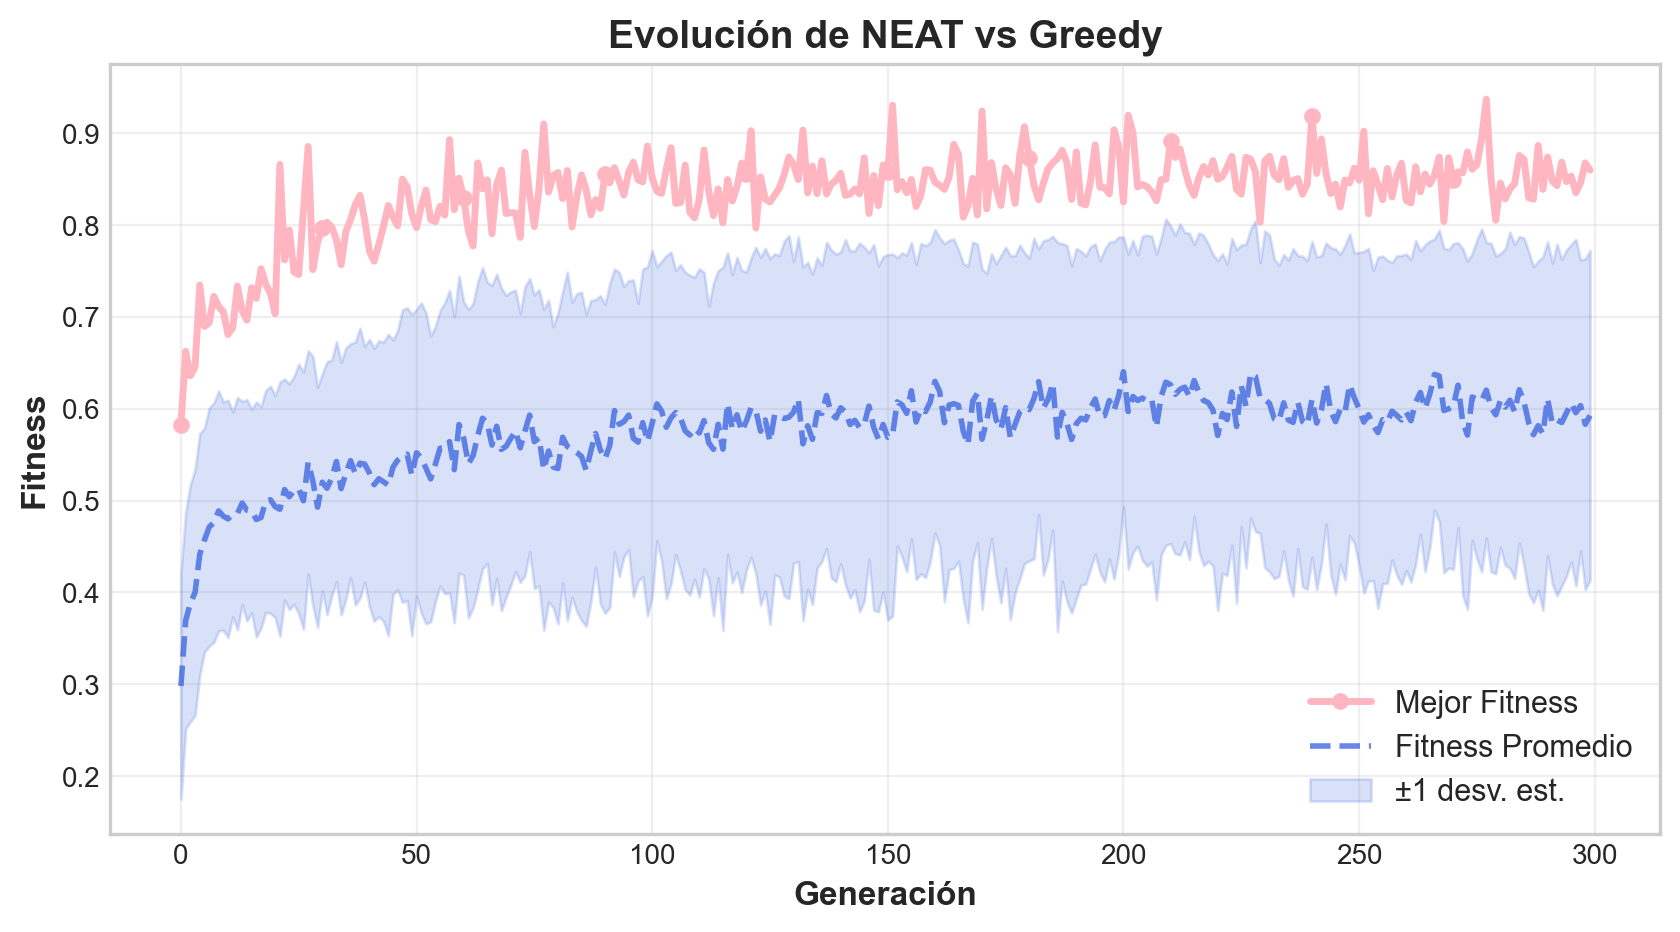
\includegraphics[width=0.75\textwidth]{figures/neat_evolution_heuristic_greedy.png}
\caption[Evolución de fitness NEAT multi-seed]{Evolución del fitness de NEAT multi-seed real vs greedy durante 300 generaciones. Se observa convergencia progresiva sin sobreajuste.}
\label{fig:neat_evolution}
\end{figure}

La mejora se extiende a todos los oponentes: contra denial pasó de WR = 0.565 a 0.635 (+7\%), y contra spread se mantuvo estable en 0.634. Este hallazgo demuestra que la técnica de entrenamiento (multi-seed real) tiene mayor impacto que la cantidad de generaciones.

\section{Discusión}

\subsection{Comparativa consolidada de paradigmas}

La Tabla \ref{tab:paradigm_comparison} presenta una comparativa consolidada de los tres paradigmas evaluados, considerando rendimiento competitivo, costo computacional y características cualitativas.

\begin{table}[H]
\centering
\caption{Comparativa de paradigmas: rendimiento vs costo}
\begin{tabular}{lcccccc}
\hline
\textbf{Criterio} & \textbf{PPO} & \textbf{NEAT} & \textbf{DT (destilado)} \\
\hline
Winrate promedio & 0.604 & \textbf{0.653} & 0.608 \\
Inferencia (5k juegos) & 44s & 28s & \textbf{33s} \\
Tamaño modelo & 161 KB & \textbf{3.4 KB} & 145 KB \\
Entrenamiento & $\sim$10 min & $\sim$30 min & $<$3s (+PPO) \\
¿Requiere tuning? & No & Sí & No \\
¿Interpretable? & No & No & \textbf{Sí} \\
GPU necesaria & No & No & No \\
\hline
\end{tabular}
\label{tab:paradigm_comparison}
\end{table}

La Figura~\ref{fig:comparativa_paradigmas} presenta de forma visual la comparativa de winrate promedio de cada paradigma, y la Figura~\ref{fig:system_winrates} muestra los winrates agrupados por sistema y oponente.

\begin{figure}[H]
\centering
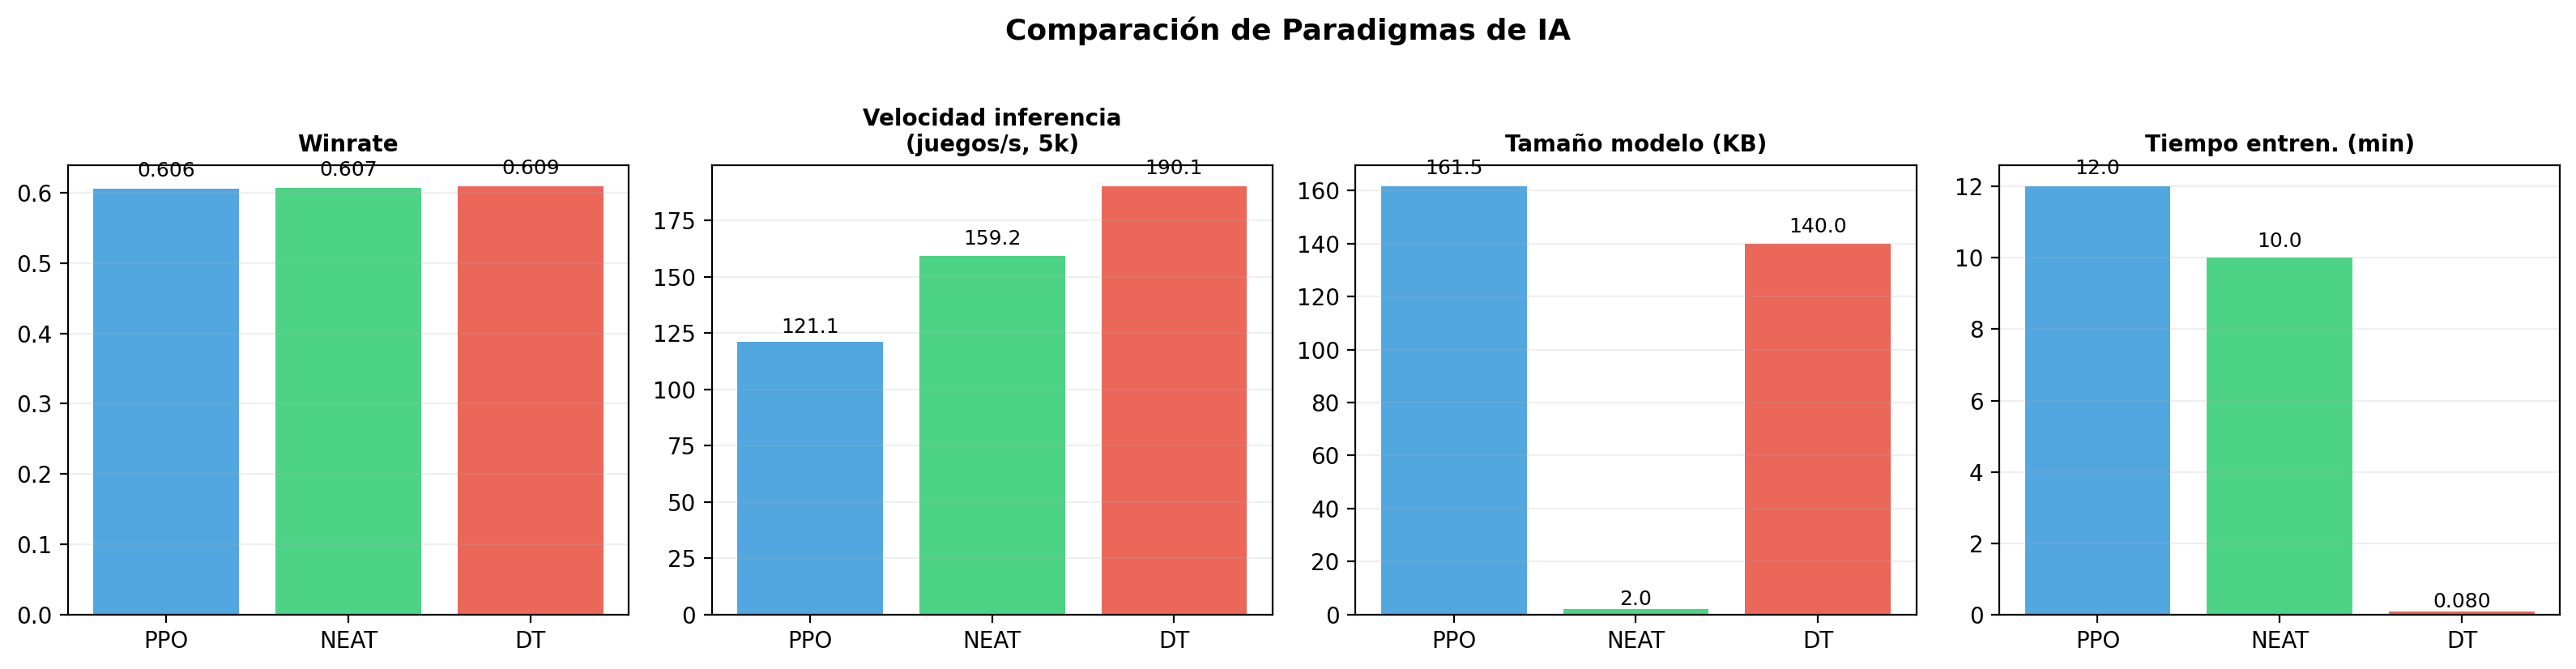
\includegraphics[width=0.8\textwidth]{figures/paradigm_comparison.png}
\caption[Comparativa consolidada de paradigmas]{Comparativa consolidada de paradigmas: winrate promedio, tiempo de entrenamiento y tamaño de modelo.}
\label{fig:comparativa_paradigmas}
\end{figure}

\begin{figure}[H]
\centering
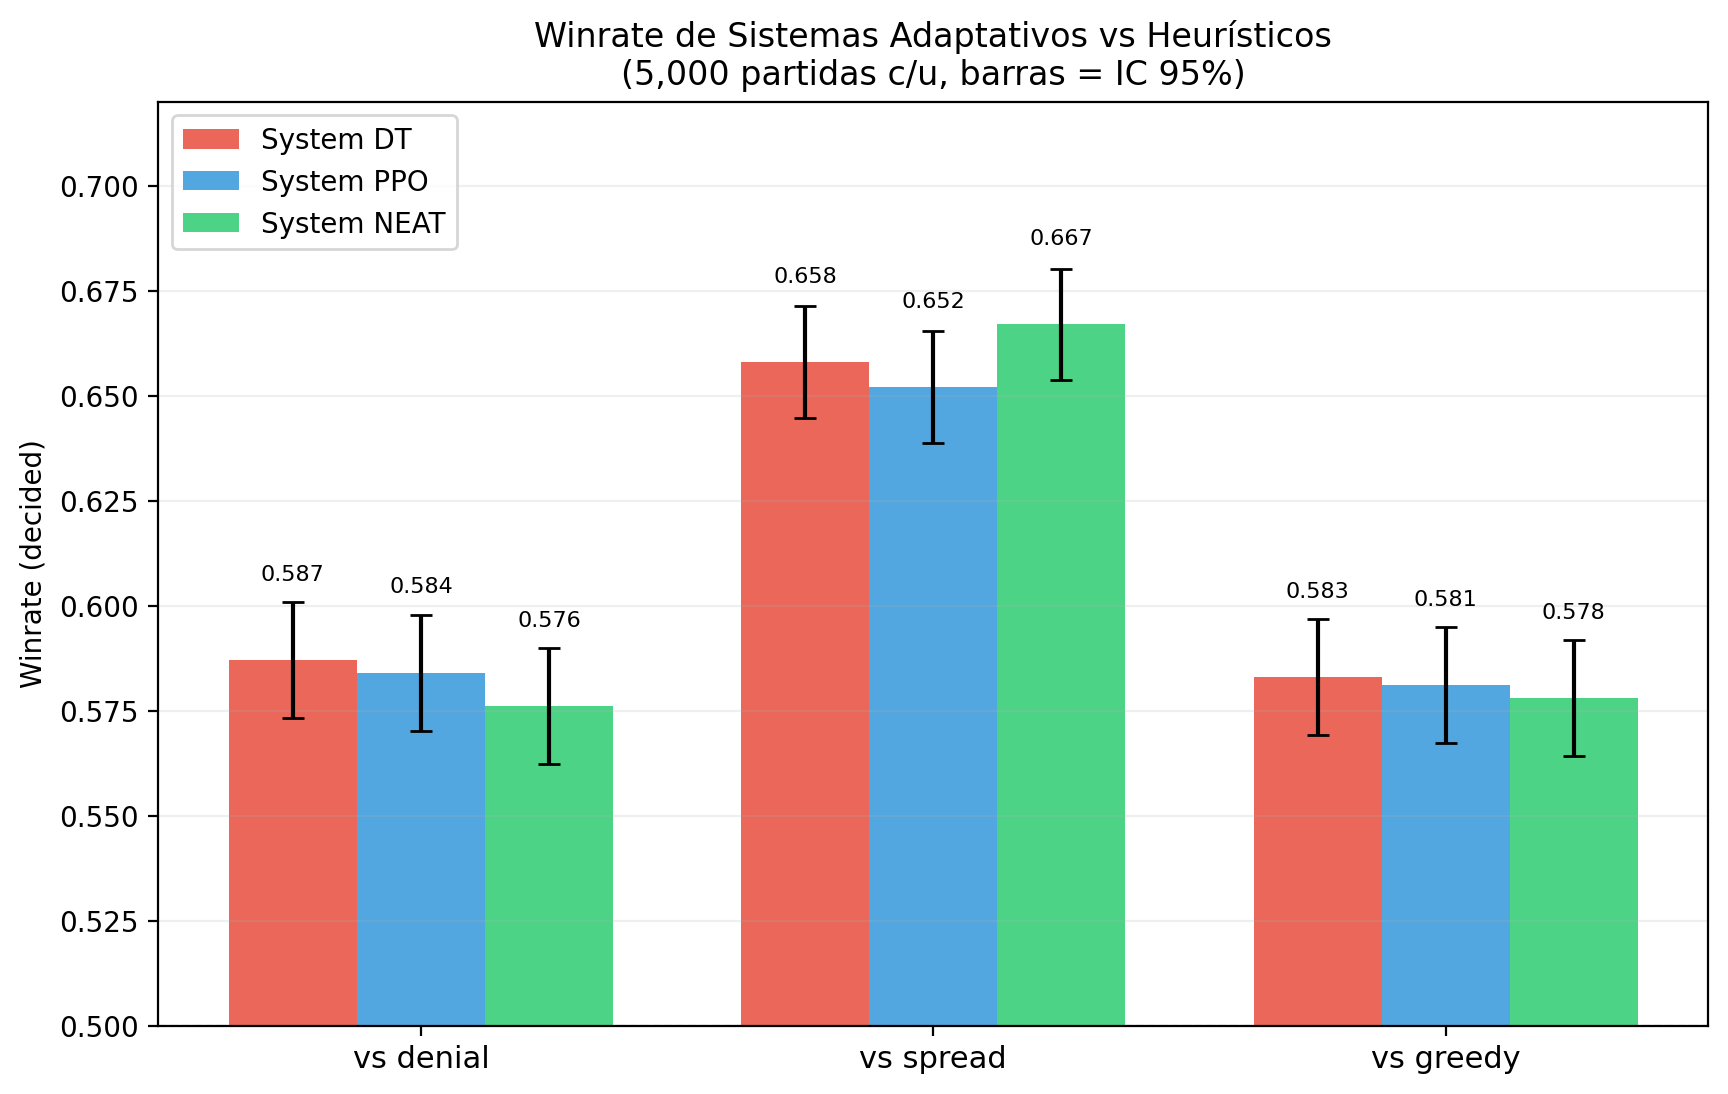
\includegraphics[width=0.8\textwidth]{figures/system_winrates_grouped.png}
\caption[Winrate por sistema y oponente]{Winrate de cada sistema adaptativo por oponente heurístico (5,000 partidas por matchup).}
\label{fig:system_winrates}
\end{figure}

\subsection{Hallazgos principales}

\begin{enumerate}
    \item \textbf{El entrenamiento en tiempo real no es viable por escasez de datos}: los tres paradigmas requieren entre 2 y 4 órdenes de magnitud más datos de los que un jugador humano genera en una sesión real (180--1,800 muestras vs. 400,000--4,590,000 requeridas). Esta brecha no se resuelve con mayor velocidad de cómputo.

    \item \textbf{El entrenamiento offline en hardware local sí es viable}: todos los modelos se entrenaron en $<$33 minutos por especialista, sin GPU, en hardware doméstico. El pipeline completo (entrenamiento + evaluación) se ejecuta en menos de 3 horas. Esto demuestra que el aprendizaje es factible cuando se dispone de un entorno de simulación acelerada.

    \item \textbf{La adaptación por selección es operativamente viable}: el mecanismo de KMeans + response table + especialistas pre-entrenados mantiene rendimiento competitivo comparable al mejor generalista fijo, con latencia de inferencia del agente inferior a 0.1 ms por turno y sin reentrenamiento en runtime. Su beneficio competitivo es limitado en Knucklebones debido a la baja diversidad estratégica del dominio.

    \item \textbf{NEAT con multi-seed alcanza el mejor rendimiento}: con WR = 0.653 (IC 95\%: [0.645, 0.660]), el sistema NEAT supera significativamente a PPO (0.604) y DT (0.608), con $p < 0.003$ en 6 de 9 comparaciones tras corrección de Bonferroni. La técnica de entrenamiento multi-seed real fue determinante para la convergencia.

    \item \textbf{La destilación preserva el rendimiento en un modelo ligero}: PPO y DT destilado son estadísticamente equivalentes ($p > 0.5$), demostrando que \textit{Behavior Cloning} preserva $>$93\% de fidelidad con un modelo interpretable, inferencia más rápida y entrenamiento instantáneo ($<$3 segundos). Esto evidencia una ruta viable para comprimir modelos entrenados offline.

    \item \textbf{Ausencia de sobreajuste}: $\Delta < 2\%$ en evaluación cruzada para todas las familias. Los agentes generalizan contra oponentes no vistos durante el entrenamiento.
\end{enumerate}

\subsection{Implicaciones}

\textbf{Sobre el aprendizaje en tiempo real}: los resultados demuestran que el entrenamiento online continuo durante la partida no es viable en hardware local con los paradigmas evaluados (PPO, NEAT, DT). La limitación principal no es la capacidad de cómputo, sino la escasez fundamental de datos: un jugador humano genera órdenes de magnitud menos muestras de las necesarias para que cualquiera de estos enfoques converja.

\textbf{Sobre la adaptación por selección}: el mecanismo de perfilado (KMeans) combinado con selección de especialistas pre-entrenados constituye una alternativa práctica demostrada. No requiere reentrenamiento en runtime, opera con latencia despreciable ($<$0.1 ms) y alcanza un rendimiento competitivo equivalente al mejor generalista fijo. En dominios con mayor diversidad estratégica (RTS, MOBA), donde un solo agente generalista no puede cubrir todos los perfiles de oponente, se esperaría un beneficio más pronunciado de este mecanismo.

\textbf{Sobre la elección de paradigma}: cuando el entrenamiento offline es la vía elegida, NEAT con multi-seed real ofrece el mejor rendimiento competitivo (WR = 0.653) con modelos ultraligeros (3.4 KB). Si se prioriza interpretabilidad o velocidad de iteración, DT destilado por \textit{Behavior Cloning} ofrece rendimiento equivalente a PPO con entrenamiento casi instantáneo.

\subsection{Limitaciones observadas}

\begin{itemize}
    \item \textbf{Dominio experimental limitado}: Knucklebones es un juego de reglas simples con espacio de acciones reducido (3 columnas). La brecha de datos podría variar en juegos con mayor complejidad, aunque probablemente se ampliaría dado que dominios más complejos requieren más datos de entrenamiento.
    \item \textbf{Oponentes heurísticos}: los oponentes de entrenamiento y evaluación son heurísticos diseñados, no jugadores humanos reales. Un estudio con jugadores humanos aportaría validez externa adicional.
    \item \textbf{Paradigmas evaluados}: se evaluaron tres paradigmas representativos (RL, neuroevolución, aprendizaje supervisado). Existen enfoques no evaluados ---como \textit{meta-learning}, \textit{few-shot learning} o aprendizaje incremental--- que podrían reducir la brecha de datos, aunque su aplicabilidad en videojuegos en hardware local permanece como pregunta abierta.
    \item \textbf{Sesión humana estimada}: la estimación de 10--100 partidas como límite de una sesión humana se basa en observación práctica y no en un estudio formal de comportamiento de usuario.
    \item \textbf{KMeans con k fijo}: no se exploró exhaustivamente el espacio de hiperparámetros del perfilador. Un clustering más fino podría mejorar la selección de especialistas.
\end{itemize}



\chapter{Conclusiones} \label{cap:conclusion}
El presente capítulo sintetiza los hallazgos principales del trabajo y responde a la pregunta central de la investigación: ¿es viable que una inteligencia artificial aprenda en tiempo real dentro de un videojuego ejecutado en hardware local? Se evalúa el cumplimiento de los objetivos planteados y se presentan las proyecciones de la investigación.

\section{Conclusiones por Objetivo}

\subsection{Medición del costo de aprendizaje}

Se midió experimentalmente el costo de entrenamiento de tres paradigmas de inteligencia artificial: PPO requirió entre 390 y 1,369 segundos y 400,000 timesteps por especialista; NEAT requirió entre 1,818 y 1,995 segundos con poblaciones de 150 genomas durante 300 generaciones y evaluación multi-seed (102 episodios por genoma); DT destilado requirió menos de 3 segundos, pero depende de un teacher PPO previamente entrenado. El perfilador KMeans se entrenó en menos de 1 minuto. Todos los entrenamientos se ejecutaron exclusivamente en CPU, en hardware doméstico, sin requerir GPU.

\subsection{Brecha entre entrenamiento offline y sesión real}

Se cuantificó la brecha de datos entre los requerimientos de entrenamiento y la disponibilidad de muestras en una sesión contra un jugador humano. Los paradigmas evaluados requieren volúmenes de datos significativamente superiores a los disponibles en una sesión real:

\begin{itemize}
    \item \textbf{PPO}: $\sim$400,000 muestras (pares estado-acción).
    \item \textbf{NEAT}: $\sim$4,590,000 episodios evaluados (300 generaciones $\times$ 150 genomas $\times$ 102 episodios).
    \item \textbf{DT}: $\sim$500,000 muestras etiquetadas (generadas por un teacher PPO).
\end{itemize}

En contraste, una partida típica de Knucklebones produce aproximadamente 18 turnos. Un jugador humano razonablemente comprometido jugaría entre 10 y 100 partidas antes de perder interés, generando entre 180 y 1,800 muestras de decisión. Esta estimación constituye un supuesto operativo conservador; el análisis de sensibilidad presentado en el Capítulo~\ref{cap:aplicacion} demuestra que la conclusión no cambia dentro de rangos razonables (incluso con 100 partidas, la brecha es superior a 222$\times$ para PPO).

La brecha resultante es de 2 a 4 órdenes de magnitud, lo cual impide que cualquiera de los tres paradigmas converja a una política funcional durante una sesión de juego real.

\subsection{Adaptación por selección como alternativa}

Se diseñó e implementó un mecanismo de adaptación por selección que combina perfilado no supervisado (KMeans con ventana temporal de 6 turnos), tablas de respuesta (response tables) y especialistas pre-entrenados. Este mecanismo opera sin reentrenamiento en tiempo de ejecución, con latencia de inferencia del agente inferior a 0.1 milisegundos por turno y latencia total del ciclo de decisión (incluyendo middleware HTTP) inferior a 10 milisegundos. El sistema adaptativo alcanzó rendimiento equivalente al mejor generalista fijo, validando la adaptación por selección como alternativa viable al entrenamiento online continuo.

\subsection{Desempeño de los sistemas adaptativos}

Los tres sistemas adaptativos alcanzaron winrates entre 0.604 y 0.653 contra oponentes heurísticos. El análisis estadístico (z-test con corrección de Bonferroni) reveló que:

\begin{itemize}
    \item \textbf{NEAT es significativamente superior}: con WR = 0.653 (IC 95\%: [0.645, 0.660]), supera a PPO (0.604) y DT (0.608) con $p < 0.003$ en 6 de 9 comparaciones. La técnica de entrenamiento multi-seed real fue determinante para la convergencia de NEAT.
    \item PPO y DT destilado son estadísticamente equivalentes ($p > 0.5$), y el DT ofrece ventajas prácticas: inferencia rápida, interpretabilidad y entrenamiento instantáneo.
    \item No se detectó sobreajuste en ninguna familia ($\Delta < 3\%$ en evaluación cruzada).
\end{itemize}

\subsection{Diseño de la plataforma experimental}

Se logró diseñar e implementar una arquitectura modular tipo \textit{plug-and-play} que separa la lógica del videojuego de los agentes de IA. El entorno \texttt{KnucklebonesEnv} actúa como fuente única de verdad de reglas. La arquitectura permite intercambiar agentes sin modificar el motor, centralizar la extracción de características y estandarizar el registro de métricas. Se implementó un middleware HTTP/JSON que conecta los agentes Python con el videojuego Unity, verificando su funcionamiento con latencia total inferior a 10 milisegundos por turno.

\section{Conclusión General}

El objetivo central de esta investigación fue evaluar la viabilidad de entrenar inteligencias artificiales en tiempo real dentro de un entorno de ejecución completamente offline, es decir, sin depender de infraestructura en la nube ni de servidores externos. Los resultados demuestran que el entrenamiento online continuo durante la interacción con el usuario, en hardware local estándar, no es viable con los paradigmas de aprendizaje evaluados (PPO, NEAT, DT). La limitación principal no es la capacidad de cómputo, sino la escasez fundamental de datos: un usuario genera entre 2 y 4 órdenes de magnitud menos muestras de las necesarias para que cualquiera de estos enfoques converja a una política funcional.

Este hallazgo tiene implicaciones que trascienden el dominio de los videojuegos. Cualquier sistema informático que requiera adaptación en tiempo real con recursos locales ---sistemas de recomendación embebidos, asistentes interactivos, interfaces adaptativas, dispositivos IoT con capacidad de aprendizaje--- enfrenta la misma restricción fundamental: el volumen de interacciones que un usuario genera en una sesión típica es insuficiente para entrenar modelos de aprendizaje automático convencionales.

No obstante, los resultados demuestran que existen alternativas prácticas que sí resultan viables bajo restricciones de ejecución offline:

\begin{enumerate}
    \item \textbf{Entrenamiento offline previo al despliegue}: los agentes alcanzan rendimiento competitivo (WR 60--65\%) entrenando fuera de la interacción con el usuario, sin GPU, en menos de 33 minutos por modelo. Esta estrategia es aplicable a cualquier dominio donde se disponga de un simulador o de datos históricos.

    \item \textbf{Adaptación por selección en tiempo de ejecución}: mediante clasificación del usuario (perfilado con KMeans), tablas de respuesta y especialistas pre-entrenados, el sistema se adapta sin reentrenar, con latencia de inferencia inferior a 0.1 ms. Este enfoque permite personalización en tiempo real sin el costo del entrenamiento continuo.

    \item \textbf{Recolección de datos en tiempo real para reentrenamiento posterior}: una alternativa intermedia consiste en registrar las interacciones durante las sesiones reales y utilizarlas para actualizar los modelos de forma periódica, fuera de línea. Esta estrategia aprovecha datos reales sin imponer el costo del entrenamiento durante la interacción, y es aplicable a sistemas que requieran mejora continua basada en el comportamiento observado de usuarios reales.

    \item \textbf{Compresión de modelos mediante destilación}: modelos complejos (PPO) se transforman en modelos livianos e interpretables (DT) mediante \textit{Behavior Cloning}, preservando $>$93\% de fidelidad con entrenamiento instantáneo. Esto facilita el despliegue en dispositivos con recursos limitados.
\end{enumerate}

La neuroevolución (NEAT) con entrenamiento multi-seed real alcanzó el mejor rendimiento competitivo (WR = 0.653), demostrando que la técnica de entrenamiento tiene un impacto mayor que la complejidad del algoritmo. Este hallazgo refuerza la importancia de la metodología experimental rigurosa y la iteración sobre el protocolo de entrenamiento.

La arquitectura modular diseñada ---con separación estricta entre la lógica del sistema y los agentes de IA--- no solo facilita la evaluación reproducible, sino que constituye un patrón de diseño transferible a otros dominios. La integración mediante middleware HTTP/JSON demuestra que es posible desacoplar completamente el sistema principal de los módulos de inteligencia artificial, habilitando actualizaciones independientes y experimentación controlada.

En síntesis, la respuesta a la pregunta central de esta investigación no es binaria. El aprendizaje online continuo no es viable con los paradigmas convencionales debido a la brecha de datos, pero la adaptación parcial mediante selección de especialistas pre-entrenados, combinada con recolección de datos para reentrenamiento periódico, constituye una alternativa práctica demostrada que puede aplicarse tanto a videojuegos como a cualquier sistema informático que requiera adaptación en tiempo real con recursos de cómputo locales.

\section{Trabajo Futuro}

Dentro de las principales líneas de trabajo futuro se encuentran:

\begin{itemize}
    \item \textbf{Exploración de técnicas de bajo costo de datos}: investigar enfoques de \textit{meta-learning}, \textit{few-shot learning} o aprendizaje incremental que podrían reducir la brecha de datos necesarios, acercando la viabilidad del entrenamiento online en sesiones reales.
    \item \textbf{Reentrenamiento offline con datos de sesión}: una alternativa intermedia consiste en recolectar datos de las partidas contra jugadores humanos y utilizarlos para reentrenar los modelos fuera de línea, actualizando los especialistas periódicamente. Esta aproximación mantiene la viabilidad demostrada del entrenamiento offline y aprovecha datos reales.
    \item \textbf{Modificación de NEAT para adaptación incremental}: explorar la posibilidad de ajustar genomas NEAT existentes con pocas evaluaciones adicionales, partiendo de un modelo pre-entrenado en lugar de entrenar desde cero.
    \item \textbf{Evaluación con jugadores humanos}: ejecutar partidas con personas reales para validar la transferencia de las políticas aprendidas, medir la experiencia subjetiva de juego y confirmar la estimación de datos disponibles por sesión.
    \item \textbf{Dominios con mayor diversidad estratégica}: aplicar el marco experimental a juegos con mayor variedad de estilos de juego (RTS, juegos por turnos con más acciones), donde la adaptación por selección podría aportar mayor beneficio.
    \item \textbf{Optimización del perfilador}: investigar clustering adaptativo, variación del número de clusters y features de perfilado más discriminantes.
\end{itemize}

\section{Reflexiones}

El desarrollo de este proyecto permitió adquirir y consolidar competencias relevantes en múltiples áreas:

\begin{itemize}
    \item \textbf{Machine Learning aplicado}: diseño, entrenamiento y evaluación de modelos de RL, neuroevolución y aprendizaje supervisado.
    \item \textbf{Diseño experimental}: control de variables, reproducibilidad, tests estadísticos y análisis de significancia.
    \item \textbf{Ingeniería de software}: arquitectura modular, patrones de diseño, separación de responsabilidades y automatización de pipelines.
    \item \textbf{Análisis de datos}: métricas, visualización, intervalos de confianza y correcciones para comparaciones múltiples.
\end{itemize}

Un aprendizaje significativo fue que la pregunta original ---si una IA puede aprender en tiempo real dentro de un entorno ejecutado localmente--- no tiene una respuesta binaria. El entrenamiento online continuo no es viable con los paradigmas convencionales evaluados debido a la brecha de datos, pero la adaptación parcial mediante selección de especialistas pre-entrenados, perfilado del usuario y recolección de datos para reentrenamiento posterior sí lo es, y produce resultados competitivos.

Esta distinción entre ``aprendizaje online pleno'' y ``adaptación online por selección'' resultó ser el hallazgo más relevante de la investigación. Si bien este trabajo se centró en el dominio de videojuegos, el patrón identificado podría ser relevante para otros sistemas que enfrenten restricciones similares de recursos locales y volumen de datos por sesión.


\bibliography{bibliografia}


\appendix

\chapter{Plan de Trabajo y Carta Gantt}
\label{anexo:Gantt}
El plan de trabajo se estructuró en fases iterativas que reflejan la evolución real del proyecto. La planificación inicial contempló un prototipo FPS exploratorio, el cual fue abandonado por razones metodológicas en favor de un entorno controlado basado en Knucklebones.

Las fechas ancla verificables del proyecto son:
\begin{itemize}
    \item 18/04/2025: primera propuesta conceptual aprobada con observaciones.
    \item 03/05/2025: segunda propuesta refinada y aceptada por el comité.
    \item 11/06/2025: presentación del prototipo FPS con movimiento básico en Unity.
    \item 20/02/2026: contexto técnico y arquitectura modular consolidados.
    \item 06/03/2026: estado post-implementación completa con modelos entrenados y evaluados.
\end{itemize}

Las Figuras~\ref{fig:gantt_parte1}, \ref{fig:gantt_parte2} y \ref{fig:gantt_parte3} presentan la Carta Gantt del proyecto completo, dividida en tres períodos para mayor legibilidad.

% ════════════════════════════════════════════════════════════════
% PARTE 1: Abril – Julio 2025 (Fases 1–2)
% ════════════════════════════════════════════════════════════════
\begin{figure}[!ht]
\centering
\begin{ganttchart}[
    hgrid,
    vgrid={*{1}{draw=none}, dotted},
    x unit=0.85cm,
    y unit title=0.45cm,
    y unit chart=0.45cm,
    title height=1,
    bar height=0.6,
    bar top shift=0.2,
    group/.append style={draw=black, fill=blue!30},
    bar/.append style={fill=blue!50},
    milestone/.append style={fill=red!70, shape=diamond, inner sep=1.2pt},
    title label font=\footnotesize,
    bar label font=\footnotesize,
    group label font=\footnotesize\bfseries,
    milestone label font=\footnotesize\itshape,
]{1}{8}

\gantttitle{2025}{8} \\
\gantttitle{Abr}{2}
\gantttitle{May}{2}
\gantttitle{Jun}{2}
\gantttitle{Jul}{2} \\

% FASE 1
\ganttgroup{Fase 1: Formulaci\'{o}n}{1}{4} \\
\ganttbar{Propuesta conceptual}{1}{1} \\
\ganttmilestone{Aprobada (18/04)}{1} \\
\ganttbar{Revisi\'{o}n bibliogr\'{a}fica}{1}{6} \\
\ganttbar{Segunda propuesta}{2}{3} \\
\ganttmilestone{Aceptada (03/05)}{3} \\

% FASE 2
\ganttgroup{Fase 2: Prototipo FPS}{4}{6} \\
\ganttbar{Escena Unity}{4}{5} \\
\ganttbar{Jugabilidad base}{5}{6} \\
\ganttmilestone{Demo FPS (11/06)}{5}

\end{ganttchart}
\caption[Carta Gantt --- Parte 1 (abril--julio 2025)]{Carta Gantt -- Parte 1 (abril--julio 2025): formulaci\'{o}n del proyecto y prototipado exploratorio del FPS. Los diamantes rojos indican hitos verificables.}
\label{fig:gantt_parte1}
\end{figure}

% ════════════════════════════════════════════════════════════════
% PARTE 2: Agosto – Diciembre 2025 (Fases 3–4)
% ════════════════════════════════════════════════════════════════
\begin{figure}[!ht]
\centering
\begin{ganttchart}[
    hgrid,
    vgrid={*{1}{draw=none}, dotted},
    x unit=0.85cm,
    y unit title=0.45cm,
    y unit chart=0.45cm,
    title height=1,
    bar height=0.6,
    bar top shift=0.2,
    group/.append style={draw=black, fill=blue!30},
    bar/.append style={fill=blue!50},
    milestone/.append style={fill=red!70, shape=diamond, inner sep=1.2pt},
    title label font=\footnotesize,
    bar label font=\footnotesize,
    group label font=\footnotesize\bfseries,
    milestone label font=\footnotesize\itshape,
]{1}{10}

\gantttitle{2025}{10} \\
\gantttitle{Ago}{2}
\gantttitle{Sep}{2}
\gantttitle{Oct}{2}
\gantttitle{Nov}{2}
\gantttitle{Dic}{2} \\

% FASE 3
\ganttgroup{Fase 3: Reformulaci\'{o}n}{1}{4} \\
\ganttbar{An\'{a}lisis de riesgos FPS}{1}{2} \\
\ganttbar{Cambio de alcance}{2}{3} \\
\ganttbar{Dise\~{n}o Knucklebones}{3}{4} \\

% FASE 4
\ganttgroup{Fase 4: Arquitectura}{4}{10} \\
\ganttbar{Formalizaci\'{o}n matem\'{a}tica}{4}{5} \\
\ganttbar{Simulador Gym}{5}{7} \\
\ganttbar{Arquetipos heur\'{i}sticos}{6}{8} \\
\ganttbar{Features can\'{o}nicas}{7}{9} \\
\ganttbar{Arquitectura 3 capas}{8}{10}

\end{ganttchart}
\caption[Carta Gantt --- Parte 2 (agosto--diciembre 2025)]{Carta Gantt -- Parte 2 (agosto--diciembre 2025): reformulaci\'{o}n metodol\'{o}gica del alcance hacia Knucklebones y dise\~{n}o de la arquitectura modular.}
\label{fig:gantt_parte2}
\end{figure}

% ════════════════════════════════════════════════════════════════
% PARTE 3: Enero – Marzo 2026 (Fases 5–8)
% ════════════════════════════════════════════════════════════════
\begin{figure}[!ht]
\centering
\begin{ganttchart}[
    hgrid,
    vgrid={*{1}{draw=none}, dotted},
    x unit=1.4cm,
    y unit title=0.45cm,
    y unit chart=0.45cm,
    title height=1,
    bar height=0.6,
    bar top shift=0.2,
    group/.append style={draw=black, fill=blue!30},
    bar/.append style={fill=blue!50},
    milestone/.append style={fill=red!70, shape=diamond, inner sep=1.2pt},
    title label font=\footnotesize,
    bar label font=\footnotesize,
    group label font=\footnotesize\bfseries,
    milestone label font=\footnotesize\itshape,
    today=5,
    today label=Hoy,
    today label font=\footnotesize\itshape,
    today rule/.style={draw=red!60, ultra thick, dashed},
]{1}{6}

\gantttitle{2026}{6} \\
\gantttitle{Ene}{2}
\gantttitle{Feb}{2}
\gantttitle{Mar}{2} \\

% FASE 5
\ganttgroup{Fase 5: Entrenamiento}{1}{4} \\
\ganttbar{PPO (3 especialistas)}{1}{2} \\
\ganttbar{Destilaci\'{o}n PPO$\to$DT}{2}{3} \\
\ganttbar{NEAT multi-seed}{2}{4} \\
\ganttbar{KMeans + Response Tables}{3}{4} \\
\ganttmilestone{Arq. consolidada (20/02)}{3} \\

% FASE 6
\ganttgroup{Fase 6: Evaluaci\'{o}n}{3}{5} \\
\ganttbar{Evaluaci\'{o}n cruzada}{3}{4} \\
\ganttbar{An\'{a}lisis estad\'{i}stico}{4}{5} \\
\ganttbar{Ablation study}{4}{5} \\

% FASE 7
\ganttgroup{Fase 7: Integraci\'{o}n Unity}{3}{5} \\
\ganttbar{Middleware Flask}{3}{4} \\
\ganttbar{Bridge Unity--Python}{4}{5} \\
\ganttmilestone{Sistema completo (06/03)}{5} \\

% FASE 8
\ganttgroup{Fase 8: Redacci\'{o}n}{4}{6} \\
\ganttbar{Informe final}{4}{6} \\
\ganttbar{Correcciones}{5}{6}

\end{ganttchart}
\caption[Carta Gantt --- Parte 3 (enero--marzo 2026)]{Carta Gantt -- Parte 3 (enero--marzo 2026): entrenamiento de modelos, evaluaci\'{o}n experimental, integraci\'{o}n con Unity y redacci\'{o}n del informe. La l\'{i}nea roja punteada indica la fecha de cierre.}
\label{fig:gantt_parte3}
\end{figure}


\end{document}
